% created on 2019-12-13
% @author : bmazoyer

%% Lines to compile only this capter
% \documentclass[11pt, twoside, a4paper, openright]{report}
% \usepackage[utf8]{inputenc}
% \DeclareUnicodeCharacter{223C}{~}

%Bibliography style
% \usepackage[square, numbers]{natbib}
% \usepackage[round]{natbib}
% \usepackage{biblatex}
% \bibliographystyle{unsrtnat}
% \bibliographystyle{unsrt}
% \bibliographystyle{plain}
% \bibliographystyle{aa}
% \usepackage[backend=bibtex,style=authoryear,natbib=true]{biblatex} 
\usepackage[
backend=biber,
style=authoryear,
citestyle=authoryear,
url=false
]{biblatex}
\addbibresource{../source/library.bib}

\usepackage[T1]{fontenc}
\usepackage[french]{babel}
\usepackage{csquotes}  % used for citations (recommended when using biblatex)
%\usepackage{helvet}
%\renewcommand{\familydefault}{\sfdefault}
\usepackage{mathptmx}
\usepackage{amssymb}
\usepackage{geometry} 
\usepackage{xcolor}
\usepackage[absolute,overlay]{textpos}
\usepackage{graphicx}
\usepackage{lipsum}
\usepackage[explicit]{titlesec}
\usepackage{lmodern}
\usepackage{color}
\usepackage{array}
\usepackage{mathtools}
\usepackage{caption}
\usepackage{multicol}
\usepackage{booktabs}
\usepackage{enumitem}
\usepackage{hyperref}
\usepackage{afterpage}
\usepackage{emptypage}
\usepackage{setspace}
\usepackage{pgffor}
    \setlength{\columnseprule}{0pt}
    \setlength\columnsep{10pt}
\usepackage[francais,nohints]{minitoc}
    \setcounter{minitocdepth}{3}
 
 %https://la-bibliotex.fr/2019/02/03/ecrire-les-nombres-et-les-unites-avec-latex/   
\usepackage{siunitx}
% \sisetup{
%     detect-all,
%      output-decimal-marker={,},
%      group-minimum-digits = 3,
%      group-separator={~},
%      number-unit-separator={~},
%      inter-unit-product={~},
%      list-separator = {, },
%      list-final-separator = { et },
%      range-phrase = --,
%      separate-uncertainty = true,
%      multi-part-units = single,
%      list-units = single,
%      range-units = single
%     }
\usepackage{physics}
\usepackage{isotope}

\usepackage[perpage]{footmisc} % to reset the counter of footnote each page

    
\usepackage{fancyhdr}			% Entête et pieds de page. Doit être placé APRES geometry
\pagestyle{fancy}		% Indique que le style de la page sera justement fancy
%\lfoot[\thepage]{} 		% gauche du pied de page
%\cfoot{} 			% milieu du pied de page
%\rfoot[]{\thepage} 
\fancyfoot{} % vide le pied~de~page
\fancyfoot[LE,RO]{\thepage}
\fancyfoot[LO,CE]{}% droite du pied de page
\fancyhead{}	
\fancyhead[LE]{\leftmark}	
\fancyhead[RO]{\rightmark}

\fancypagestyle{plain}{%
\fancyhf{} % vide l’en-tête et le pied~de~page.
\fancyfoot[LE,RO]{\thepage} % numéro de la page en cours en gras% et centré en pied~de~page.
\renewcommand{\headrulewidth}{0pt}
\renewcommand{\footrulewidth}{0pt}}



% Premiere page des chapitres
\newlength\chapnumb
\setlength\chapnumb{3cm}
 
\titleformat{\chapter}[block] {
  \normalfont}{}{0pt} { %police
    \parbox[b]{\chapnumb}{
      \fontsize{120}{110}\selectfont\thechapter} %taille du chiffre
      \parbox[b]{\dimexpr\textwidth-\chapnumb\relax}{
        \raggedleft 
        \hfill{\bfseries\Huge#1}\\ %taille du titre
        \rule{\dimexpr\textwidth-\chapnumb\relax}{0.4pt} %ligne de separation
  }
}
 
 %premiere page chapitre non numerote (remerciement, table des matieres ...)
 
\titleformat{name=\chapter,numberless}[block]
{\normalfont}{}{0pt}
{   
    \parbox[b]{\dimexpr\textwidth}{%   
    \hfill{\bfseries\Huge#1}\\
  \rule{\dimexpr\textwidth}{0.4pt}}}
    
 %   \titleformat{name=\chapter,numberless}[block]
%{\normalfont}{}{0pt}
%{\parbox[b]{\chapnumb}{%
%   \mbox{}}%
%  \parbox[b]{\dimexpr\textwidth-\chapnumb\relax}{%
%    \raggedleft%
%    \hfill{\bfseries\Huge#1}\\
%    \rule{\dimexpr\textwidth-\chapnumb\relax}{0.4pt}}}


%%%    SIunitx
\sisetup{locale = FR,
  % inter-unit-product=\ensuremath{\cdot},
  inter-unit-product=\ensuremath{\,},
  per-mode=reciprocal,
  separate-uncertainty = true,
  detect-all
}
\DeclareSIUnit{\Mpc}{Mpc}
\DeclareSIUnit{\kpc}{kpc}
\DeclareSIUnit{\Gpc}{Gpc}
\DeclareSIUnit{\h}{\textit{h}~}
\DeclareSIUnit{\perh}{\textit{h}^{-1}\,}

%%% Geometry
\geometry{
left=20mm,
top=30mm,
right=20mm,
bottom=30mm
}

%%% Color
\definecolor{bordeau}{rgb}{0.3515625,0,0.234375}

%%% Commands
\newcommand{\Nmocks}{\num{30}}
\newcommand{\hMpc}{h^{-1}\,\mathrm{Mpc}}
\newcommand{\hGpc}{h^{-1}\,\mathrm{Gpc}}
\newcommand{\kms}{\mathrm{km\,s^{-1}}}

\newcommand{\lya}{Ly$\alpha$}
\newcommand{\lyb}{Ly$\beta$}
\newcommand{\lyalya}{Ly$\alpha$(Ly$\alpha$)}
\newcommand{\lyalyb}{Ly$\alpha$(Ly$\beta$)}

\newcommand{\lrf}{\lambda_{\rm RF}}
\newcommand{\kpar}{k_{\parallel}}
\newcommand{\apar}{\alpha_{\parallel}}
\newcommand{\rpar}{r_{\parallel}}
\newcommand{\aperp}{\alpha_{\perp}}
\newcommand{\rperp}{r_{\perp}}
\newcommand{\kperp}{k_{\perp}}

\newcommand{\blya}{b_{\rm Ly\alpha}}
\newcommand{\betalya}{\beta_{\rm Ly\alpha}}
\newcommand{\blyb}{b_{\rm Ly\alpha}}
\newcommand{\betalyb}{\beta_{\rm Ly\beta}}
\newcommand{\dlya}{d_{\rm Ly\alpha}}
\newcommand{\bhcd}{b_{\rm HCD}}
\newcommand{\betahcd}{\beta_{\rm HCD}}
\newcommand{\Fhcd}{F_{\rm HCD}}
\newcommand{\Lhcd}{L_{\rm HCD}}

\newcommand{\imin}{i_{\rm min}}
\newcommand{\imax}{i_{\rm max}}
\newcommand{\jmin}{j_{\rm min}}
\newcommand{\jmax}{j_{\rm max}}

\newcommand{\xioned}{\xi_{\rm 1d}}
\newcommand{\DHub}{D_{H}}
\newcommand{\DM}{D_{M}}

\newcommand{\omegam}{\Omega_M}
\newcommand{\omegac}{\Omega_C}
\newcommand{\omegab}{\Omega_B}
\newcommand{\omegan}{\Omega_\nu}
\newcommand{\omegal}{\Omega_\Lambda}
\newcommand{\omegak}{\Omega_k}
\newcommand{\orad}{\Omega_R}
\newcommand{\ogam}{\Omega_\gamma}
\newcommand{\lcdm}{$\Lambda$CDM}

\newcommand{\picca}{\texttt{picca}}

%%% Rem's command
\newcommand\blankpage{%
    \null
    \thispagestyle{empty}%
    \addtocounter{page}{-1}%
    \newpage}
  
% Command to set up a particular alignment for a cell in tabular :
% \myalign{c}{foo} for instance
\newcommand*{\myalign}[2]{\multicolumn{1}{#1}{#2}}
 
\renewcommand{\thesection}{\arabic{section}}

% Romain
\newcommand{\cRM}[1]{\MakeUppercase{\romannumeral #1}}	% Capital
\newcommand{\cRm}[1]{\textsc{\romannumeral #1}}	% Petit majuscule
\newcommand{\crm}[1]{\romannumeral #1}
% Siècle %
\newcommand{\siecle}[1]{\cRm{#1}\textsuperscript{e}~siècle}



% Thesis title
\newcommand{\PhDTitle}{Les forêts \lya{} du relevé eBOSS : comprendre les fonctions de corrélation et les systématiques} 

% Name
\newcommand{\PhDname}{Thomas Etourneau} 

% Change this variable if you add or remove chapters
\newcommand*{\NumOfChapters}{6}

% Change this variable if you add or remove appendices
\newcommand*{\NumOfAppendices}{2}

% PDF metadata
\hypersetup{
	pdfauthor={\PhDname},
	pdfsubject={Manuscrit de thèse de doctorat},
	pdftitle={\PhDTitle}
}


% \begin{document}
%%

\graphicspath{ {../figures/mocks/} }

\chapter{Développement des mocks}
\minitoc
\newpage
\thispagestyle{fancy}

Dans ce chapitre, nous présentons la construction des \emph{mocks} : des spectres de quasars simulés, dont les forêts \lya{}
sont corrélées entre elles et avec le champ de quasars sous-jacent.
%  et le champ de quasars possèdent les bonnes fonctions d'auto corrélation et de corrélation croisée.
% des simulations qui visent à reproduire les données d'eBOSS et de DESI. Ces mocks, nommés \texttt{SaclayMocks} et présentés dans \textcite{CITE:mocks}, sont le c{\oe}ur de ce manuscrit.
Ces mocks visent à reproduire les données d'eBOSS et de DESI. Ils sont nommés \texttt{SaclayMocks} et présentés dans \textcite{Etourneau2020}.
Le code est écrit en Python\footnote{https://www.python.org/} et se trouve en accès libre sur GitHub\footnote{https://github.com/igmhub/SaclayMocks}. L'utilisation de ces mocks et leur validation seront présentés dans les chapitres suivants.

\section{Objectifs des mocks}
% Les mocks s'inscrivent dans le projet DESI, et sont utilisés dans l'analyse finale des données eBOSS \autocite{CITE:dr16}.
Contrairement à ce qu'on appelle les simulations, les mocks ne contiennent pas de physique à proprement parler : ils ne sont pas utilisés afin de déduire des paramètres astrophysiques. Certaines simulations, les simulations hydrodynamiques, permettent de mesurer des effets astrophysiques, comme par exemple le biais de l'hydrogêne ou du \lya{}. Mais ces simulations sont très couteuses car elles nécessitent de modéliser les effets physiques qui affectent les paramètres mesurés.
Les mocks, quant à eux, sont conçus afin de répliquer rapidement un jeu de données, dans le but de tester l'analyse qui sera appliquée sur ces données.
% Dans le cas de l'analyse \lya{} d'eBOSS et de DESI, les mocks sont utilisés afin
Les mocks sont donc utilisés afin
\begin{itemize}[label=$\bullet$]
\item de vérifier la mesure des paramètres $\apar{}$, $\aperp{}$ : cette mesure est-elle non biaisée ?
\item d'identifier les potentielles systématiques : la présence de métaux et d'HCD dans les données est-elle bien modélisée ? Affecte-t-elle la mesure de $\apar{}$, $\aperp{}$ ?
\item de tester la matrice de distorsion : la distorsion de la fonction de corrélation due à l'ajustement du continuum du quasar est-elle correctement prise en compte par la matrice de distorsion ?
\item de vérifier l'estimation de la matrice de covariance : la matrice de covariance, calculée à partir des données, est-elle bien estimée ?
\end{itemize}
La production et l'analyse d'un grand nombre de mocks permet de répondre précisément à ces questions. Ces mocks sont donc nécessaires pour pouvoir valider l'analyse menée sur les données.

\paragraph{}
Les mocks décrits dans ce manuscrit s'inscrivent dans les projets eBOSS et DESI. Ils sont utilisés dans l'analyse \lya{} des données complète d'eBOSS \autocite{DuMasdesBourboux2020}, et seront utilisés dans l'analyse \lya{} de DESI.
L'objectif de ces mocks est donc de répliquer au mieux les données \lya{} d'eBOSS et de DESI. Ces relevés couvrent un volume de plusieurs dizaines de \si{\cubic\Gpc}, et les échelles sondées grâce au \lya{} descendent jusqu'à la centaine de \si{\kpc}. Les mocks nécessitent donc de reproduire un volume immense, avec une bonne résolution.
Les simulations dites \emph{N-corps} sont des simulations qui traitent le problème à N corps.
% Elles sont initialisées avec une distribution de matière noire, représentée par des macro-particules de masse $\sim 10^{9} M_{\odot}$, à un redshift élevé ($z > 100$).
Elles sont initialisées à un redshift élevé ($z > \num{100}$), avec une distribution de matière noire représentée par des macro-particules.
% Généralement, environ $(\num{10000})^3$ macro-particules sont présentes dans ces simulations.
Actuellement, les simulations les plus performantes utilisent environ $(\num{10000})^3$ macro-particules.
La masse de ces particules dépend du volume simulé. Par exemple, la simulation Outer Rim \autocite{Heitmann2019} simule un volume d'environ $(\SI{4}{\Gpc})^3$, et les particules possèdent une masse $\sim 10^{9} M_{\odot}$.
Puis, à chaque pas de temps, ces macro-particules sont déplacées en considérant uniquement les interactions gravitationnelles. Le champ de matière initial évolue ainsi jusqu'à $z=0$. Ces simulations sont très utiles pour étudier les effets de la gravité à grande échelle. Cependant elles ne sont pas adaptées à notre utilisation : afin d'avoir la résolution et le volume requis, la simulation nécessiterait beaucoup trop de macro-particules pour être réalisable dans un temps raisonnable.

Les simulations hydrodynamiques fonctionnent de la même manière que les simulations N-corps. Elles incluent, en plus des macro-particules de matière noire, la physique baryonique présente dans le milieu galactique. Les baryons sont aussi représentés par des macro-particules. Afin de résoudre l'intérieur des galaxies, les macro-particules utilisées possèdent une masse plus faible que dans le cas des simulations N-corps. En contrepartie, le volume simulé est plus petit. Dans le cas des simulations hydrodynamiques, la densité, la pression et la tempéature sont tracées dans chaque cellule. Certains effets astrophysiques, comme les supernovae ou les AGN peuvent aussi être présents. 
% Cependant, ces simulations ne sont pas non plus adaptées à notre utilisation car le volume d'univers simulé est bien trop petit : quelques dizaines de \si{\perh\cubic\Mpc}.
Ces simulations nécessitent encore plus de temps de calcul que les simulations à N-corps. Elles ne sont donc pas non plus adaptées à notre utilisation.

% Ainsi, avoir un grand volume et une grande résolution requiert l'utilisation des \emph{champs aléatoires gaussiens} (GRF pour Gaussian Random Field). 
Ainsi, seuls les \emph{champs aléatoires gaussiens} (GRF pour Gaussian Random Field) permettent de générer un grand volume avec une bonne résolution.
Ce sont des champs qui en chaque point prennent une valeur aléatoire selon une statistique gaussienne.
Une fois générés, il est possible de donner à ces champs n'importe quelle fonction de corrélation, en utilisant la transformation de Fourier.
%Les GRF sont donc idéaux pour simuler le champ de matière à grande échelle.
Ces champs sont utilisés notament dans les simulations à N-corps, afin de fournir les conditions 
Cependant, l'utilisation des GRF ne donne pas accès aux non-linéarités qui peuvent émerger dans l'évolution des simulations N-corps et hydrodynamiques. La seule information provient de la fonction de corrélation que l'on applique au GRF.
Mais cela est entièrement suffisant pour l'utilisation que nous en avons dans ce manuscrit : nous générons un champ gaussien destiné à simuler le champ d'absorption \lya{} et le champ de quasars, dont les fonctions d'auto corrélation et de corrélation croisée sont choisies afin de correspondre à ce qui est observé dans les données.


\section{Construction des mocks}
Dans cette section, nous détaillons comment les mocks sont générés.
Nous présentons d'abord la génération des champs de densité,
% puis de ces champs de densité, comment sont tirés les quasars.
puis comment les quasars sont tirés à partir de ces champs de densité.
%Nous expliquons ensuite comment, de la position de chaque quasar, nous créons sa ligne de visée.
Nous expliquons ensuite comment nous calculons la densité le long de la ligne de visée de chaque quasar.
% Enfin, nous présentons comment de la densité le long de la ligne de visée nous calculons la fraction de flux transmis et comment nous tirons les HCD.
Enfin, nous présentons comment cette densité est transformée en fraction de flux transmis, et comment nous tirons les HCD.


\subsection{Les champs de densité}
\label{subsec:densityfields}
La première étape dans la création des mocks est de générer les boîtes qui contiennent le champ de densité $\delta$. D'abord, un GRF est généré dans une boite de $\num{2560}\times\num{2560}\times\num{1536}$ voxels, chaque voxel faisant  $d_{cell}^3 = (\SI{2.19}{\perh\Mpc})^3$.
Afin que le champ $\delta$ possède la bonne fonction de corrélation, une transformation de Fourier 3D\footnote{Nous utilisons la librairie pyFFTW (https://github.com/pyFFTW/pyFFTW), une adaptation python de la librairie FFTW (http://www.fftw.org/).} est appliquée sur la boîte, puis la boîte $\delta_k$ ainsi obtenue est multipliée par
\begin{equation}
  \sqrt{\frac{P(k)}{d_{cell}^3}} \; ,
\end{equation}
% \textbf{où $P(k)$ est le spectre de puissance désiré. Ce procédé garanti que le champ $\delta_k$ suive le spectre de puissance $P(k)$. Il est ensuite possible d'obtenir la boîte $\delta$ dans l'espace réel grâce à une transformation de Fourier inverse de la boîte $\delta_k$.}
où $P(k)$ est le spectre de puissance désiré. Il est ensuite possible d'obtenir la boîte $\delta$ dans l'espace réel grâce à une transformation de Fourier inverse de la boîte $\delta_k$. Ce procédé garanti que le champ $\delta$ suive le spectre de puissance $P(k)$. 
% Le GRF pourrait être tiré directement dans l'espace $k$ mais nous ne perdons pas beaucoup de temps CPU\footnote{Le temps CPU (Central Processing Unit) désigne le temps utilisé par les processeurs d'une machine pour exécuter un code.} à procéder comme cela.
Le GRF pourrait être tiré directement dans l'espace $k$. Dans ce cas, il nous faut tirer deux champs gaussiens : un pour la partie réelle, et un autre pour la partie imaginaire. La transformation de Fourier prenant moins de temps que la génération du champ aléatoire, nous préférons générer le champ dans l'espace réel plutôt que dans l'espace $k$.
% Nous distingons ici deux champs : le champ utilisé pour tirer les quasars, et le champ utilisé pour créer l'absorption \lya{}. Ces deux champs requièrent deux spectres de puissance différents, et donc deux boîtes de densité différentes.
Dans la suite nous décrivons les différentes boîtes nécessaires à la construction des mocks : les boîtes champs utilsées pour tirer les quasars, la boîte utilisée pour créer l'absorption \lya{}, ainsi que les boîtes de vitesse et de gradient de vitesse. Afin de garantir leur corrélation, toutes ces boîtes sont construites à partir de la même boîte initial $\delta_k$.

\subsubsection{Les quasars}
\label{subsubsec:boiteqso}
Afin de construire un relevé de quasars corrélés, nous tirons les quasars selon le champ dans l'espace réel $\delta_{\textsc{QSO}}$, construit à partir de $\delta_k$. Une première solution serait de tirer les quasars dans les voxels dont le champ $\delta_{\textsc{QSO}}$ est supérieur à un certain seuil. Cette solution produit une fonction de corrélation correcte aux grandes échelles, mais pas aux petites.
% En effet, comme expliqué précédemment, l'utilisation des GRF ne permet pas de capturer l'évolution non linéaire du champ de matière, qui se manifeste aux petites échelles.
En effet, comme montré dans \textcite{Font-Ribera2012a}, les objets tirés aux endroits où la densité est supérieure à un certain seuil suivent la fonction de corrélation de la densité sous-jacente, avec un biais qui dépend du seuil choisi, si et seulement si la fonction de corrélation est petite devant 1. La fonction de corrélation ainsi obtenue est correcte, sauf pour les petites échelles pour lesquelles la fonction de corrélation est importante.
% Plutôt que de modéliser ces non-linéarités, nous considérons une seconde solution : nous considérons que les quasars suivent une distribution log-normale. Ceci permet d'obtenir une meilleure corrélation aux petites échelles.
Une solution alternative consiste à considérer que les quasars suivent une distribution log-normale. Ceci permet d'obtenir une meilleure corrélation aux petites échelles.
% Comme expliqué précédemment, l'utilisation des GRF ne permet pas de capturer l'évolution non linéaire du champ de matière. Plutôt que de modéliser ces non-linéarités, nous considérons que les quasars suivent une distribution log-normale.
Ce choix est souvent fait pour simuler des relevés de galaxies \autocite{Agrawal2017}, et est en accord avec ce qui est observé dans les données \autocite{Clerkin2016}.
% Ainsi, au lieu de placer les quasars dans les voxels qui possèdent une densité plus élevé qu'un certain seuil, nous tirons les quasars dans chaque voxel avec une probabilité
% Ainsi, dans chaque voxel, les quasars sont tirés avec une probabilité
Nous optons donc pour cette seconde solution. Ainsi, les quasars sont tirés dans chaque voxel avec une probabilité
\begin{equation}
  \label{eq:proba_qso}
  P \propto \mathrm{e}^{\delta_q} \; ,
\end{equation}
où $\delta_q$ est le champ de densité dans le voxel considéré.
Comme montré par \textcite{coles_lognormal_1991}, afin que les quasars suivent la fonction de corrélation $\xi(r)$, le champ $\delta_q$ doit suivre la fonction de corrélation 
\begin{equation}
  \label{eq:lognormal}
  \xi_q(r) = \ln(1+\xi(r)) \; .
\end{equation}
Nous verrons section~\ref{subsec:qso} que, de manière à obtenir un relevé synthétique de quasars dont le biais dépend de $z$, nous utilisons trois boîtes qui suivent des distributions log-normales, à des redshifts différents. La probabilité pour tirer les quasars dépend de l'interpolation entre ces 3 boîtes.
% Ces champs sont construits aux redshits $z_1 = \num{1.9}$, $z_2 = \num{2.75}$, et $z_3 = \num{3.6}$.
Pour chacune des boîtes, nous partons du spectre de puissance de la matière $P_{\mathrm{matière}}(k)$ à $z=0$, fourni par Camb~\autocite{Lewis1999}. Nous multiplions ensuite ce spectre de puissance par $(b_{\textsc{QSO}}(z_i) G(z_i))^2$, où $i \in [1\, ; 2\, ; 3]$. A l'aide de la transformation de Fourier, nous calculons la fonction de corrélation $\xi_{i}(r)$. Puis, nous déterminons le spectre de puissance $P_{\textsc{QSO},i}(k)$, à appliquer à la boîte $\delta_k$, comme la transformée de Fourier de $\xi_{\textsc{QSO},i}(r) = \ln(1+\xi_i(r))$ (équation~\ref{eq:cf_tf2}).
Une fois les trois spectres de puissances $P_{\textsc{QSO},i}(k)$ obtenus, nous construisons 3 boîtes
\begin{equation}
  \delta_{k,i}(k)  = \delta_k(k) \sqrt{\frac{P_{\textsc{QSO},i}(k)}{V_{cell}}} \; ,
\end{equation}
où $\delta_k$ est le GRF dans l'espace de Fourier. Une fois ces 3 boîtes construites, nous appliquons à chacune d'entre elle une transformation de Fourier inverse afin d'obtenir les boîtes $\delta_{\textsc{QSO}, i}$. Ces boîtes seront interpolées en $z$, puis les quasars seront ensuite tirés avec une probabilité $\propto \exp(\delta_{\textsc{QSO}}(z))$, où $\delta_{\textsc{QSO}}$ est la boîte interpolée. Nous expliquons cette étape dans la section~\ref{subsec:qso}.


\subsubsection{Le champ \lya{}}
Afin de construire le champ d'absorption \lya{}, nous avons besoin du champ de densité de l'hydrogène neutre. Comme expliqué dans la section~\ref{subsec:lya}, la fraction de flux transmis $F$ est reliée à la profondeur obtique $\tau$ par
\begin{equation}
  F = \exp(- \tau) \; .
\end{equation}
De plus, la formule FGPA (Fluctuating Gunn Peterson Approximation) permet de relier la profondeur optique $\tau$ au contraste de densité $\delta$ à $z = 0$ :
\begin{equation}
  \label{eq:fgpa1}
  \tau(z) = a(z) \exp(b(z) G(z) \delta) \;
\end{equation}
Les paramètres $a$ et $b$ sont des paramètres à ajuster afin d'obtenir le bon biais du \lya{} et la bonne transmission moyenne $\overline F$. Leur détermination est décrite dans la section~\ref{sec:tuning}. Le facteur de croissance $G$ prend en compte l'évolution avec le redshift du champ de densité $\delta$. Ainsi il nous suffit de construire un GRF qui suit la fonction de corrélation à $z=0$ pour simuler le champ d'absorption du \lya{}. Pour ce faire, nous partons de la même boîte $\delta_k$ utilisée pour construire les 3 boîtes log-normales des quasars. Ceci garanti la corrélation croisée entre les quasars et le champ d'absorption \lya{}. Le spectre de puissance de la matière $P_{\mathrm{matière}}(k)$ à $z=0$ est ensuite appliqué à la boîte $\delta_k$. Enfin, nous obtenons la boîte de densité $\delta_{\mathrm{matière}}$ à $z = 0$ qui servira au calcul du champ d'absorption du \lya{} en effectuant la transformée de Fourier de la boîte
\begin{equation}
  \delta_{k, matière}(\vec k)  = \delta_k(\vec k) \sqrt{\frac{P_{\mathrm{matière}}(\vec k)}{V_{cell}}} \; .
\end{equation}


\subsubsection{Les champs des vitesses}
\label{subsubsec:vitesses}
Afin d'inclure les RSD dans nos mocks, nous simulons aussi le champ des vitesses. A l'ordre linéaire, le champ des vitesses $v_{k,n}$ dans l'espace $k$ selon la direction $\vec u_{n}$, avec $n \in [\textsc{x} \, ;\textsc{y} \, ;\textsc{z}]$, est relié au champ de densité $\delta_k$ par la relation (voir équation 9.18 et 9.20 de \textcite{Dodelson2003})
\begin{equation}
  \label{eq:v1}
  v_{k,n}(\vec k) = \frac{ik_n}{k^2}  a H f \delta_{k}(\vec k) \; .
\end{equation}
% Le champ $\delta_{k, matière}$ est le champ de fluctuation de la matière à $z = 0$ dans l'espace $k$ calculé précédemment.
% Il est fréquent
% (\#prov approximation réaliste ? mettre une source ; j'ai demandé a Etienne : theorie lineaire pas de biais, c'est ce qui est utilisé pour la reconstruction. Y a des gens qui regardent dans les simu nbody si y a un biais des vitesses qui apparait, dans les simus eBOSS y a rien de convainquant, mais le papier est tres peu fournit a ce sujet)
% de considérer que le champ de vitesse des traceurs est le même que celui de la matière sous-jacente. Autrement dit, le champ de vitesse des traceurs est non biaisé.
En théorie linéaire, les traceurs sont considérés avoir la même vitesse que le champ de matière sous-jacent. Autrement dit, le champ de vitesse des traceurs est non biaisé. Nous adoptons ici cette hypothèse.
En ce qui concerne les quasars, nous simulons les RSD en déplaçant chaque quasar proportionnellement à sa vitesse le long de la ligne de visée (équation~\ref{eq:delta_z}). Dans ce but, nous calculons les trois boîtes de vitesses $v_{k,\textsc{x}}$, $v_{k,\textsc{y}}$ et $v_{k,\textsc{z}}$, comme
\begin{equation}
  \label{eq:v2}
  v_{k, n}(\vec k, z) = \frac{- i k_n}{k^2} H(z) \frac{dG}{dz}(z) \delta_{k, matière}(\vec k) \; ; \hspace{0.5cm} n \in [\textsc{x} \, ; \textsc{y} \, ; \textsc{z}] \; .
\end{equation}
Ces boîtes sont construites pour $z = 0$. Cette équation est équivalente à l'équation~\ref{eq:v1}, car
\begin{equation}
  f=\frac{d \ln G}{d \ln a}=\frac{a}{G} \frac{dG}{da}=-\frac{1}{aG}\frac{dG}{dz}
\end{equation}
Comme précédemment, la boîte $\delta_{k, matière}$ est la même que celle utilisée pour construire les boîtes $\delta_{\textsc{QSO},i}$ des quasars et la boîte $\delta_{\mathrm{matière}}$ utilisée pour le \lya{}, ceci afin de garantir la correspondance entre la densité des traceurs et leurs vitesses particulières. A l'aide d'une transformation de Fourier inverse, nous obtenons les trois boîtes de vitesse à $z=0$ dans l'espace réel $v_{\textsc{x}}$, $v_{\textsc{y}}$ et $v_{\textsc{z}}$. Le calcul pour obtenir la vitesse parallèle $v_{\parallel}$ à un redshift $z$ est décrit dans la section~\ref{subsec:qso}.
% A l'aide d'une transformation de Fourier, nous obtenons chaque champ de vitesse dans l'espace réel $v_x$, $v_y$ et $v_z$, ce qui nous permet de calculer la vitesse le long de la ligne de visée
% \begin{equation}
%   v_{\parallel}(\vec r) = \frac{\vec r \cdot \vec v}{|| \vec r ||} \; .
% \end{equation}

Concernant le champ d'absorption \lya{}, les RSD sont prises en compte par une modification de la formule FGPA. Pour ce faire, nous avons besoin du gradient de vitesse $\eta_{\parallel}$ à $z=0$.
Nous utilisons la définition donnée dans l'équation 2.2 de \textcite{Arinyo-i-Prats2015} :
\begin{equation}
  \eta = - \frac{1}{aH} \frac{\partial v_p}{\partial x_p} \; ,
\end{equation}
où $\eta$ est le gradient sans dimension de la vitesse $v_p$ le long de la ligne de visée, et $x_p$ est la coordonnées comobile le long de cette ligne de visée.
En utilisant la définition précédente, et l'équation~\ref{eq:v1}, nous obtenons le gradient $\eta_{nm}$ de la vitesse $v_n$ selon la direction $\vec u_m$ en fonction du champ $\delta_k$ :
% Le gradient $\eta_{nm}$ selon la direction $\vec u_m$ de la vitesse $v_n$ est défini comme
\begin{equation}
  \label{eq:eta1}
  \eta_{nm}(\vec k) = \frac{k_n k_m}{k^2} f \delta_k(\vec k) \; .
\end{equation}
Cette équation permet de retrouver la formule de kaiser :
\begin{align}
  \label{eq:kaiser5}
  \delta_k^s(\vec k) &= \delta_k(\vec k) + \eta_{\parallel}(\vec k) \; ,   \\
                     &= (1 + f \mu_k^2) \delta_k(\vec k)  \; .  \nonumber
\end{align}
  La boîte $\delta_k$ utilisée est le GRF initial, afin de garantir les corrélations entre les différents champs. A l'aide d'une transformation de Fourier inverse, nous obtenons\footnote{Lors de la construction des 6 boîtes de gradients de vitesses, nous omettons volontairement le facteur $f(z=0)$ de l'équation~\ref{eq:eta1}. Ce facteur $f$ manquant sera pris en compte lors de l'ajout de la dépendance en redshift (voir section~\ref{subsubsec:rsdlya})} les 6 boîtes de gradients de vitesses  à $z = 0$ dans l'espace réel $\eta_{\textsc{xx}}$, $\eta_{\textsc{yy}}$, $\eta_{\textsc{zz}}$, $\eta_{\textsc{xy}}$, $\eta_{\textsc{yz}}$ et $\eta_{\textsc{xz}}$.
% (\#prov: mettre la fin de la section dans une footnote ou un appendix ?)Nous construisons donc 6 boîtes de gradients de vitesse, à $z=0$, comme
% \begin{equation}
%   \label{eq:eta2}
%   \eta_{nm}(\vec k) = \frac{k_n k_m}{k^2} \delta_k(\vec k) \; ; \hspace{0.5cm} (n,m) \in [\textsc{x}, \textsc{y}, \textsc{z}]^2 \; .
% \end{equation}
% La boîte $\delta_k$ utilisée est le GRF initial, afin de garantir les corrélations entre les différents champs. Nous omettons volontairement le facteur $f(z=0)$ à ce stade. Il sera pris en compte lors de l'ajout de la dépendance en redshift (voir section~\ref{subsubsec:rsdlya}). A l'aide d'une transformation de Fourier, nous obtenons les 6 boîtes de gradients de vitesses  à $z = 0$ dans l'espace réel $\eta_{\textsc{xx}}$, $\eta_{\textsc{yy}}$, $\eta_{\textsc{zz}}$, $\eta_{\textsc{xy}}$, $\eta_{\textsc{yz}}$ et $\eta_{\textsc{xz}}$.


% Nous calculons d'abord les 6 champs
% \begin{equation}
%   \eta_{ij}(\vec k) = \frac{- k_i k_j}{k^2} f \delta_{k, matière}(\vec k) \; ; \hspace{0.5cm} (i,j) \in [x, y, z]^2 \; .
% \end{equation}
% % Le champ $\eta_{\parallel}$ est donné par
% % \begin{equation}
% %   \eta_{\parallel}(\vec r) = \frac{r_i \eta_{ij} r_j}{r^2}
% % \end{equation}


% \paragraph{}
% blablabla
% \begin{equation}
%   \theta(k) = - f \delta(k) \;
% \end{equation}

% \begin{align}
%   v_k(z) &= \frac{-i k_{\parallel}}{k^2} \frac{H(z)}{G(z)} \frac{dG}{dz} \delta_k(z)\\
%          &= \frac{k_{\parallel}}{k^2} \dot a f \delta_k
% \end{align}
% \begin{equation}
%   \eta_{ij} = \frac{k_ik_j}{k^2} \delta
% \end{equation}
% \begin{equation}
%   v_n(k, z) = \frac{-ik_n}{k^2} \frac{H(z)}{G(z)}\frac{dG}{dz} \delta_k(z)
% \end{equation}
% Ce qui donne :
% \begin{align}
%   \eta_{nm}(k,z) &= \frac{k_nk_m}{k^2} \frac{H(z)}{G(z)}\frac{dG}{dz} \delta_k(z) \\
%                  &= \frac{k_nk_m}{k^2} (-af)H(z) \delta_k(z)
% \end{align}


\subsection{Le relevé de quasars}
\label{subsec:qso}
% Une fois tous ces champs construits, nous définissons la géométrie du relevé. Les boîtes $\num{2560}\times\num{2560}\times\num{1536}$, où \num{1536} correspond à la dimension de l'axe de la ligne de visée (dénommé $Z$ dans la suite), sont placées à un redshift central $z_0 = 1.70975268202$. Leur dimension selon cet axe permet de couvrir les redshifts $1.3 < z < 3.6$. L'observateur est considéré être à $z=0$. Il se trouve au centre dans le plan $(X,Y)$, et les boîtes sont placés à une ascension droite $\alpha_0$ et une déclinaison $\delta_0$ (voir équation~\ref{eq:radec}).
Une fois toutes ces boîtes construites, nous définissons la géométrie du relevé. Les boîtes, d'une taille $\num{2560}\times\num{2560}\times\num{1536}$ selon les axes $\textsc{x}$, $\textsc{y}$ et $\textsc{z}$ respectivement, sont placées à un redshift central $z_0 = \num{1.71}$, et à une ascension droite $\alpha_0$ et une déclinaison $\delta_0$ (voir équation~\ref{eq:radec}). Leurs dimensions permettent de couvrir les redshifts $\num{1.3} < z < \num{3.6}$.
Cette limite basse est choisie de manière à pouvoir inclure les absorptions du CIV. Comme indiqué dans la section~\ref{sec:selection_forets}, le pixel d'absorption de plus bas redshift dans la région \lya{}  se trouve à $z = \num{1.96}$. Si cette absorption est causée par du CIV, l'absorbeur se situe à un redshift $z = (1+\num{1.96}) \lambda_{\mathrm{Ly}\alpha} / \lambda_{CIV} - 1 \sim \num{1.32}$.
Enfin, l'observateur est considéré être à $z=0$, au centre du plan $(\textsc{x},\textsc{y})$.

Afin d'obtenir un biais des quasars qui dépend du redshift, nous pouvons modifier l'équation~\ref{eq:proba_qso} et inclure une facteur $\alpha(z)$ qui prend en compte l'évolution avec le redshift du champ $\delta_q$ associé aux quasars :
\begin{equation}
  \label{eq:proba_qso2}
  P \propto \exp(\alpha(z)\delta_q) \; ,
\end{equation}
où $\alpha(z)$ est donné par
\begin{equation}
  \alpha(z) = \frac{b_{\textsc{QSO}}(z) (1+z_0)}{b_{\textsc{QSO}}(z_0)(1+z)} \; ,
\end{equation}
et $z_0$ est le redshift auquel est construit le champ log-normal $\delta_q$, avec $b_{\textsc{QSO}}$ son biais.
  La paramétrisation que nous utilisons pour le biais des quasars est donnée dans l'équation~\ref{eq:b_qso}.
  La fonction de corrélation $\xi_i$ à un redshift $z_i$ est obtenue à partir de l'équation~\ref{eq:lognormal}, et s'exprime comme
  \begin{equation}
    \label{eq:lognormal2}
    \xi_i = \exp(\alpha^2(z_i) \ln (1 + \xi_0)) - 1 \; ,
  \end{equation}
  où $\xi_0$ est la fonction de corrélation à $z_0 = \num{2.33}$, obtenue comme la transformation de Fourier du spectre de puissance $P_{\mathrm{matière}}(k)$ à $z=0$ fourni par Camb, et multipliée par le facteur de croissance $G$ et le biais des quasars $b_{\textsc{QSO}}$ au redshit $z_0$.
  Dans la limite où $\xi_0 \ll 1$ ou $|1 - \alpha | \ll 1$, nous obtenons comme souhaité $\xi_i = \alpha^2(z_i) \xi_0$.
\begin{figure}
  \centering
  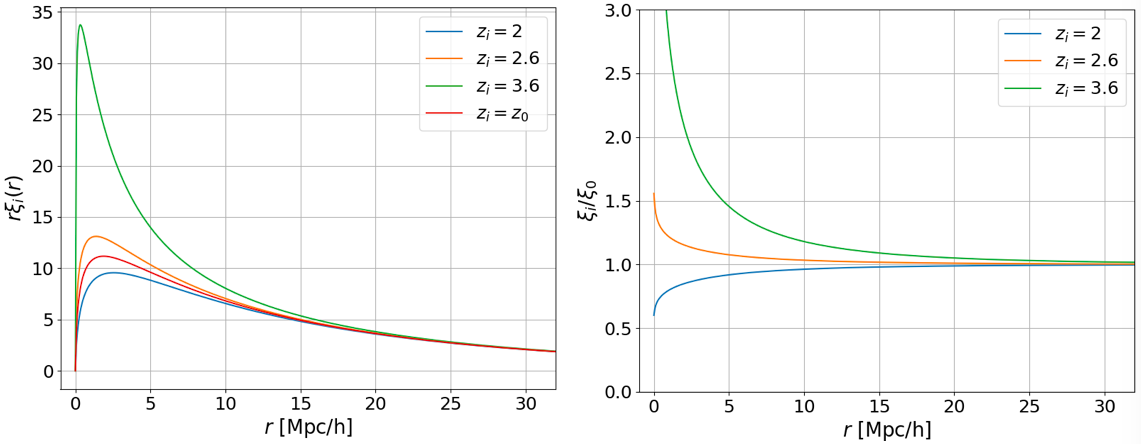
\includegraphics[scale=0.4]{qsolognormal1}
  \caption{Gauche : fonctions de corrélation $\xi_i$ obtenues à partir de l'équation~\ref{eq:lognormal2} et normalisées par un facteur $1 / \alpha^2(z_i)$. La fonction de référence $\xi_0$ est calculée à un redshift $z_0 = \num{2.33}$. Droite : rapports $\xi_i / \alpha^2(z_i) \xi_0$.}
  \label{fig:qsolognormal1}
\end{figure}
% La figure~\ref{fig:qsolognormal1} montre les fonctions de corrélation $\xi_i$, à différents redshifts $z_i$, produites avec cette méthode.
% Ces fonctions de corrélation sont obtenues en utilisant l'approximation lognormal :
% \begin{equation}
%   \label{eq:lognormal2}
%   \xi_i(z) = \exp(\alpha^2(z_i) \ln (1 + \xi_0)) - 1 \; ,
% \end{equation}
% où $\xi_0$ est la fonction de corrélation à $z_0 = \num{2.33}$, obtenue comme la transformation de Fourier inverse du spectre de puissance $P_{\mathrm{matière}}(k)$ à $z=0$ fourni par Camb, et multipliée par le facteur de croissance $G$ et le biais des quasars $b_{\textsc{QSO}}$ au redshit $z_0$.
% Les fonctions de corrélation $\xi_i$ tracées sont normalisées par un facteur $1/\alpha^2(z_i)$ afin de pouvoir comparer leur amplitude.
La figure~\ref{fig:qsolognormal1} compare les rapports $\xi_i / \alpha^2(z_i)$ avec la fonction de corrélation de référence $\xi_0$.
Nous pouvons remarquer que plus le redshift $z_i$ est éloigné de $z_0$, et plus l'écart entre $\xi_i / \alpha^2(z_i)$ et $\xi_0$ est grand.
Ceci est d'autant plus vrai pour les petites séparations $r$, pour lesquelles $\xi_0$ n'est pas négligeable devant 1. %, et donc pour lesquelles l'approximation lognormal (équation~\ref{eq:lognormal2}) n'est plus valable.
Nous pouvons aussi remarquer sur le graphique de droite de la figure~\ref{fig:qsolognormal1} que les formes des rapports $\xi_i / \alpha^2(z_i)\xi_0$ pour $z_i > z_0$ et $z_i < z_0$ sont semblables et de signe opposé. Nous pouvons donc combiner ces fonctions de corrélation afin d'avoir un résultat plus satisfaisant.

Nous considérons donc maintenant deux champs log-normaux $\delta_{\textsc{QSO},1}$ et $\delta_{\textsc{QSO},2}$ à $z_1 = \num{2.1}$ et $z_2 = \num{3.5}$. Pour chaque champ, comme précédemment, nous construisons le champ
\begin{equation}
  \label{eq:boiteqsointerp1}
  \hat  \delta_{\textsc{QSO}, i}(z) = \exp(\alpha(z) \delta_{\textsc{QSO},i}) \; ,
  \hspace{1cm} i \in [1\, ; 2] \; ,
\end{equation}
puis, nous définissons le champ $\hat \delta_{\textsc{QSO}, 12}$ comme une interpolation linéaire des deux champs définis dans l'équation précédente :
\begin{equation}
  \label{eq:boiteqsointerp2}
  \hat \delta_{\textsc{QSO}, 12}(z) = \hat \delta_{\textsc{QSO}, 1}(z) \frac{z_2 - z}{z_2 - z_1} + \hat \delta_{\textsc{QSO}, 2}(z) \frac{z - z_1}{z_2 - z_1} \; .
\end{equation}
\begin{figure}
  \centering
  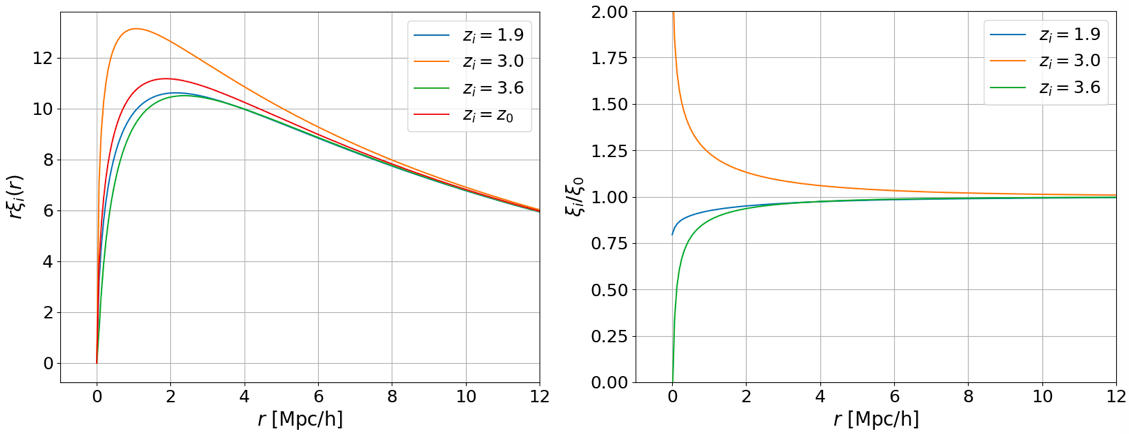
\includegraphics[scale=0.4]{qsolognormal2}
  \caption{Gauche : fonctions de corrélation $\xi_{i}(z_i)$, normalisées par un facteur $1 / \alpha^2(z_i)$ et obtenues par interpolation (orange) et extrapolation (bleu et vert) des fonctions de corrélation $\xi_1$ et $\xi_2$ à $z_1 = \num{2.1}$ et $z_2 = \num{3.5}$. Leur obtention est détaillée dans le texte. Droite : rapports $\xi_i / \alpha^2(z_i) \xi_0$. Le redshift $z = \num{3.0}$ est le redshift pour lequel la déviation par rapport à $\xi_0$ est la plus importante.}
  \label{fig:qsolognormal2}
\end{figure}
La figure~\ref{fig:qsolognormal2} montre les fonctions de corrélation normalisées $\xi_i$ qui correspondent au champ $\hat \delta_{\textsc{QSO},12}$ à différents redshifts $z_i$. Elles sont obtenues en interpolant linéairement (équation~\ref{eq:boiteqsointerp2}) les fonctions de corrélation $\xi_1$ et $\xi_2$, elles-mêmes obtenues aux redshifts $z_1$ et $z_2$ grâce aux transformations log-normales (équation~\ref{eq:lognormal2}) de $\alpha^2(z_1)\xi_0$ et $\alpha^2(z_2)\xi_0$.
Nous pouvons remarquer sur cette figure~\ref{fig:qsolognormal2} que l'écart entre les fonctions de corrélation $\xi_1$ et $\xi_2$ (en rouge) et les fonctions de corrélation interpolées est moins important que dans le cas avec un seul champ lognormal. La courbe orange montre la fonction de corrélation $\xi_i$ au redshift $z_i = \num{3.0}$ pour lequel l'écart avec $\xi_1$ et $\xi_2$ est maximal.
Comme précédemment, nous pouvons constater que l'effet entre une interpolation (orange) et une extrapolation (vert, par exemple) et similaire et de signe opposé. Afin d'affiner encore l'évolution avec le redshift du champ utilisé pour tirer les quasars, nous pouvons considérer trois champs log-normaux, et combiner une interpolation et une extrapolation obtenues à partir de ces trois champs.

Nous considérons donc finalement trois champs log-normaux $\delta_{\textsc{QSO},1}$, $\delta_{\textsc{QSO},2}$ et $\delta_{\textsc{QSO},3}$  à $z_1 = \num{1.9}$,  $z_2 = \num{2.75}$  et $z_3 = \num{3.6}$. C'est la solution qui a été choisie et implémentée dans les mocks. Ces trois champs sont stockés dans les boîtes construites dans la section~\ref{subsubsec:boiteqso}. A partir de ces trois boîtes, nous construisons les 3 boîtes $\hat \delta_{\textsc{QSO},1}$, $\hat \delta_{\textsc{QSO},2}$ et $\hat \delta_{\textsc{QSO},3}$ (équation~\ref{eq:boiteqsointerp1}), puis les deux boîtes interpolées $\hat \delta_{\textsc{QSO},12}$ et $\hat \delta_{\textsc{QSO},23}$ (équation~\ref{eq:boiteqsointerp2}). Enfin, nous construisons la boîte
\begin{equation}
  \label{eq:boiteqsointerp3}
  \hat \delta_{\textsc{QSO}}(z) = K(z) \hat \delta_{\textsc{QSO}, 12}(z) + (1 - K(z)) \hat \delta_{\textsc{QSO}, 23}(z) \; ,
\end{equation}
comme la combinaison linéaire de deux boîtes interpolées $\hat \delta_{\textsc{QSO},12}$ et $\hat \delta_{\textsc{QSO},23}$. Le paramètre $K(z)$ est déterminé tel que, pour chaque $z$, le rapport de la fonction de corrélation $\xi_{\textsc{QSO}}$, normalisée par $1/\alpha^2(z)$ et obtenue avec l'équation~\ref{eq:boiteqsointerp3}, par la fonction de corrélation $\xi_0$, vaille 1 à $r = \SI{5}{\perh\Mpc}$. La figure~\ref{fig:qsolognormal3} présente les rapports normalisés $\xi_{12}(z) / \xi_0$ (correspondant à l'interpolation, en bleu) et $\xi_{23}(z) / \xi_0$ (correspondant à l'extrapolation, en orange) au redshift $z = \num{2.38}$. La combinaison linéaire des deux (équation~\ref{eq:boiteqsointerp3}) est montrée en vert. Le redshift $z = \num{2.38}$ correspond au redshift pour lequel la différence entre $\xi_{\textsc{QSO}}$ et $\xi_0$ est la plus grande. Le graphique de droite de cette figure~\ref{fig:qsolognormal3} montre un zoom de la courbe verte. Sur ce zoom, nous pouvons voir que $\xi_{\textsc{QSO}}$ ne dévie pas de $\xi_0$ de plus de $5\times 10^{-4}$ pour $r > \SI{5}{\perh\Mpc}$.
\begin{figure}
  \centering
  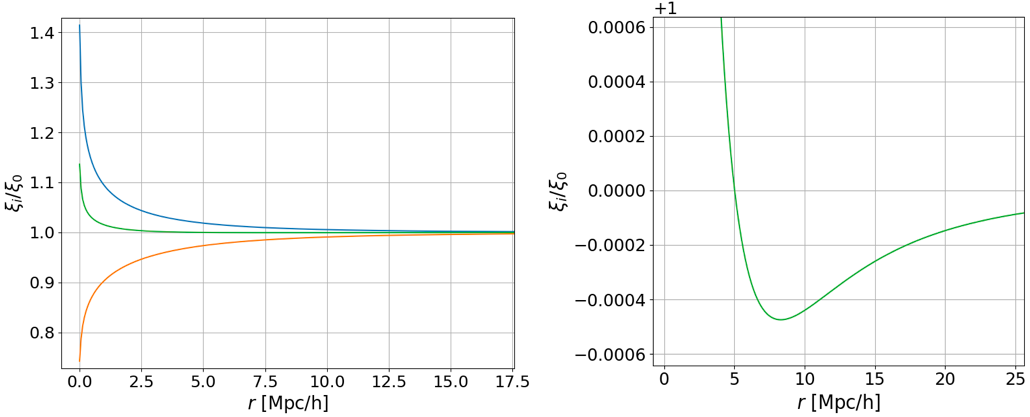
\includegraphics[scale=0.45]{qsolognormal3}
  \caption{Rapports normalisés $\xi_{12}(z) / \xi_0$ (bleu) et $\xi_{23}(z) / \xi_0$ (orange) à $z = \num{2.38}$. Pour ce redshift, $\xi_{12}$ est obtenue comme une interpolation de $\xi_1$ et $\xi_2$, et $\xi_{23}$ comme une extrapolation de $\xi_{2}$ et $\xi_{3}$. La courbe verte est obtenue comme une combinaison linéaire de $\xi_{12}$ et $\xi_{23}$. Le redshift $z = \num{2.38}$ est le redshift pour lequel la courbe verte dévie le plus de $\xi_0$. Le détail est donné dans le texte. Le graphique de droite présente un zoom de celui de gauche.}
  \label{fig:qsolognormal3}
\end{figure}



% $K(z)(r_{12} - r_{23}) + r_{23}$ vaille 1 à $r = \SI{5}{\perh\Mpc}$, où les rapports $r_{12}$ et $r_{23}$ sont définis comme
% \begin{align}
%   % r_{12}(z) &= \frac{\xi_{12}(r)}{\xi_1} \left(\frac{b_1(1+z)}{b_{QSO}(z)(1+z_1)}\right)^2 \; , \\
%   % r_{23}(z) &= \frac{\xi_{23}(r)}{\xi_1} \left(\frac{b_1(1+z)}{b_{QSO}(z)(1+z_1)}\right)^2 \; .
%   r_{12}(z) &= \frac{\xi_{12}(r)}{\xi_0} \left(\frac{b_1(1+z)}{b_{QSO}(z)(1+z_1)}\right)^2 \; , \\
%   r_{23}(z) &= \frac{\xi_{23}(r)}{\xi_0} \left(\frac{b_1(1+z)}{b_{QSO}(z)(1+z_1)}\right)^2 \; .
% \end{align}
% Ces rapports donnent la déviation de la fonction de corrélation due à l'interpolation et à l'extrapolation. La figure~\ref{fig:qsointerp3} donne $r_{12}$ (bleu), $r_{23}$ (orange) et $K(z)(r_{12} - r_{23}) + r_{23}$ (vert) à $z=\num{2.3}$, redshift pour lequel l'écart est le plus grand. La courbe verte montre que la fonction de corrélation obtenue avec le champ $\hat \delta_{\textsc{QSO}}$ ne dévie pas de plus de \SI{0.6}{\percent} de la fonction de corrélation visée à chaque redshift.




% % old
% Afin d'obtenir un biais des quasars qui dépend (\#prov dépende ?) du redshift, nous pouvons utiliser deux champs log-normaux.
% Considérons $\delta_{\textsc{QSO},1}$ et $\delta_{\textsc{QSO},2}$, deux champs log-normaux à $z_1 = \num{2.1}$ et $z_2 = \num{3.5}$.
% % Pour les redshifts $z_1 < z < z_2$, nous pouvons interpoler les deux champs
% Pour les redshifts $z < z_1$ et $z > z_2$, nous pouvons extrapoler les champs $\delta_{\textsc{QSO},1}$ et $\delta_{\textsc{QSO},2}$,
% en calculant
% \begin{equation}
%   \label{eq:boiteqsointerp1}
%   \hat \delta_{\textsc{QSO}, i}(z) = \exp(\delta_{\textsc{QSO},i} \frac{b_{\textsc{QSO}}(z) (1+z_i)}{b_{\textsc{QSO}}(z_i)(1+z)}) \; ,
%   \hspace{1cm} i \in [1; 2] \; ,
% \end{equation}
% où $b_{\textsc{QSO}}$ est le biais des quasars. Le redshift dans chaque voxel est calculé en utilisant l'équation~\ref{eq:dist_como}.
% Toutes les distances sont comobiles.
% L'équation précédente nous donne donc le champ $\hat \delta_{\textsc{QSO}, 1}$ à utiliser pour tirer les quasars lorsque $z \leq z_1$, et le champ $\hat \delta_{\textsc{QSO}, 2}$ à utiliser lorsque $z \geq z_2$.
% Pour les redshifts $z_1 < z < z_2$, nous pouvons interpoler les deux champs $\delta_{\textsc{QSO},1}$ et $\delta_{\textsc{QSO},2}$ en calculant
% \begin{equation}
%   \label{eq:boiteqsointerp2}
%   \hat \delta_{\textsc{QSO}, 12}(z) = \hat \delta_{\textsc{QSO}, 1}(z) \frac{z_2 - z}{z_2 - z_1} + \hat \delta_{\textsc{QSO}, 2}(z) \frac{z - z_1}{z_2 - z_1} \; .
% \end{equation}
% Nous pouvons alors tirer les quasars dans chaque voxel proportionnellement à l'interpolation ou l'extrapolation de ces deux champs.
% La figure~\ref{fig:qsointerp12} présente les fonctions de corrélation des champs $\hat \delta_{\textsc{QSO}, 12}$ à $z=\num{2.6}$ (vert) et à $z = \num{2.9}$ (violet), $\hat \delta_{\textsc{QSO}, 1}$ à $z=\num{1.9}$ (bleu) et $\hat \delta_{\textsc{QSO}, 2}$ à $z=\num{3.6}$ (rouge), et $\delta_{\textsc{QSO},1}$ et $\delta_{\textsc{QSO},2}$ à $z_1 = \num{2.1}$ et $z_2 = \num{3.5}$ (orange). Ces fonctions de corrélations sont corrigées de leur dépendance en redshift en divisant $\xi$ par
% \begin{equation}
%   \left(\frac{b_{\textsc{QSO}}(z) (1+z_0)}{b_{\textsc{QSO}}(z_0)(1+z)}\right)^2 \; ,
% \end{equation}
% avec $z_0 = 2.3$.
% Sur le graphique de droite de la figure~\ref{fig:qsointerp12}, nous voyons que les fonctions de corrélation obtenues par interpolation possèdent une amplitude trop grande, et celles obtenues par extrapolation une amplitude trop petite.
% % La figure~\ref{prov} présente les fonctions de corrélation des champs obtenus à un redshift $z=\num{2.6}$ (vert) et $z = \num{2.9}$ (violet) par interpolation des deux champs, à un redshift $z=\num{1.9}$ (bleu) et $z=\num{3.6}$ (rouge) par extrapolation des champs $\delta_{\textsc{QSO},1}$ et $\delta_{\textsc{QSO},2}$, et enfin, la fonction de corrélation des champs $\delta_{\textsc{QSO},1}$ et $\delta_{\textsc{QSO},2}$ à $z_1 = \num{2.1}$ et $z_2 = \num{3.5}$ (orange). Sur le graphique de droite de la figure~\ref{prov}, nous voyons que les fonctions de corrélation obtenues par interpolation possèdent une amplitude trop grande, et celles obtenues par extrapolation une amplitude trop petite.
% \begin{figure}
%   \centering
%   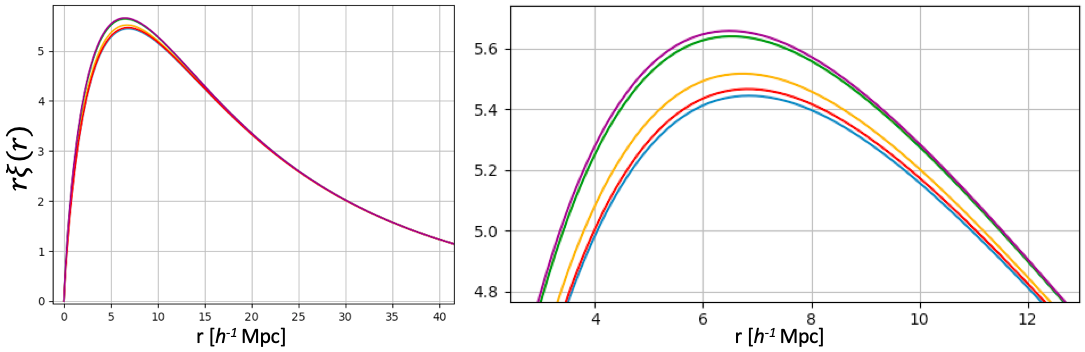
\includegraphics[scale=0.42]{qsointerp12}
%   \caption{\textbf{Fonctions de corrélation des champs $\hat \delta_{\textsc{QSO}, 12}$ à $z=\num{2.6}$ (vert) et à $z = \num{2.9}$ (violet) (\#prov refaire le plot sans le violet ?) obtenus par interpolation, des champs $\hat \delta_{\textsc{QSO}, 1}$ à $z=\num{1.9}$ (bleu) et $\hat \delta_{\textsc{QSO}, 2}$ à $z=\num{3.6}$ (rouge) obtenus par extrapolation, et des champs $\delta_{\textsc{QSO},1}$ et $\delta_{\textsc{QSO},2}$ à $z_1 = \num{2.1}$ et $z_2 = \num{3.5}$ (orange). Tous les champs sont corrigées de leur dépendance en redshift (voir texte).} Le graphique de droite présente un zoom de celui de gauche.}
%   \label{fig:qsointerp12}
% \end{figure}
% \begin{figure}
%   \centering
%   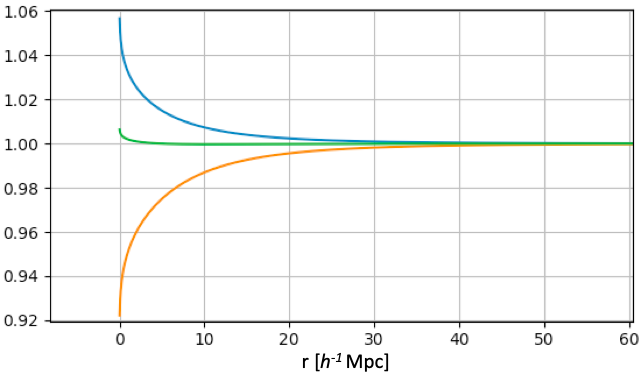
\includegraphics[scale=0.5]{qsointerp33}
%   \caption{Rapports $r_{12}$ (bleu), $r_{23}$ (orange) et $K(z)(r_{12} - r_{23}) + r_{23}$ (vert) à $z=\num{2.3}$ (voir texte). L'effet sur la fonction de corrélation dû à interpolation (bleu) compense celui dû à l'extrapolation (orange). La combinaison linéaire des deux donne la courbe verte.}
%   \label{fig:qsointerp3}
% \end{figure}
% De plus, nous pouvons voir sur la figure~\ref{fig:qsointerp3} que l'effet dû à l'interpolation (en bleu) est similaire et opposé à celui dû à l'extrapolation (orange). Ainsi, en combinant une interpolation et une extrapolation, nous obtenons une approximation bien plus satisfaisante (vert). Plutôt que d'utiliser deux champs, nous utilisons donc trois champs log-normaux à $z_1 = \num{1.9}$, $z_2 = \num{2.75}$, et $z_3 = \num{3.6}$. Ces champs sont stockés dans les boîtes construites dans la section~\ref{subsubsec:boiteqso}. Nous construisons les trois boîtes $\hat \delta_{\textsc{QSO}, i}$ définies selon l'équation~\ref{eq:boiteqsointerp1}, puis, nous créons les deux boîtes qui contiennent les champs interpolés $\hat \delta_{\textsc{QSO}, 12}$ et $\hat \delta_{\textsc{QSO}, 23}$ (équation~\ref{eq:boiteqsointerp2}). Enfin, nous construisons la boîte
% \begin{equation}
%   \label{eq:lognormal_interp}
%   % \hat \delta_{\textsc{QSO}}(z) = K(z) \left(\hat \delta_{\textsc{QSO}, 12}(z) - \hat \delta_{\textsc{QSO}, 23}(z)\right) + \hat \delta_{\textsc{QSO}, 23}(z) \; ,
%    \hat \delta_{\textsc{QSO}}(z) = K(z) \hat \delta_{\textsc{QSO}, 12}(z) + (1 - K(z)) \hat \delta_{\textsc{QSO}, 23}(z) \; ,
% \end{equation}
% où $K(z)$ est un coefficient qui varie entre 1 à $z = \num{1.9}$ et 0 à $z = 3.6$. Il est représenté sur la figure~\ref{fig:kz}. Pour chaque $z$, $K(z)$ est déterminé tel que $K(z)(r_{12} - r_{23}) + r_{23}$ vale 1 à $r = \SI{5}{\perh\Mpc}$, où les rapports $r_{12}$ et $r_{23}$ sont définis comme
% \begin{align}
%   r_{12}(z) &= \frac{\xi_{12}(r)}{\xi_1} \left(\frac{b_1(1+z)}{b_{QSO}(z)(1+z_1)}\right)^2 \; , \\
%   r_{23}(z) &= \frac{\xi_{23}(r)}{\xi_1} \left(\frac{b_1(1+z)}{b_{QSO}(z)(1+z_1)}\right)^2 \; .
% \end{align}
% Ces rapports donnent la déviation de la fonction de corrélation due à l'interpolation et à l'extrapolation. La figure~\ref{fig:qsointerp3} donne $r_{12}$ (bleu), $r_{23}$ (orange) et $K(z)(r_{12} - r_{23}) + r_{23}$ (vert) à $z=\num{2.3}$, redshift pour lequel l'écart est le plus grand. La courbe verte montre que la fonction de corrélation obtenue avec le champ $\hat \delta_{\textsc{QSO}}$ ne dévie pas de plus de \SI{0.6}{\percent} de la fonction de corrélation visée à chaque redshift.
% % end new
% %Afin de construire le catalogue de quasars, nous utilisons les trois boîtes $\delta_{\textsc{QSO}, i}$ construites précédemment, aux redshits $z_1 = \num{1.9}$, $z_2 = \num{2.75}$, et $z_3 = \num{3.6}$. Dans chaque cas, nous calculons
% % \begin{equation}
% %   \hat \delta_{\textsc{QSO}, i}(z) = \exp(\delta_{\textsc{QSO},i} \frac{b_{\textsc{QSO}}(z) (1+z_i)}{b_{\textsc{QSO}}(z_i)(1+z)}) \; ,
% %   \hspace{1cm} i \in [1, 2, 3] \; ,
% % \end{equation}
% % où $b_{\textsc{QSO}}$ est le biais des quasars. Le redshift dans chaque voxel est calculé en utilisant l'équation~\ref{eq:dist_como}. Les paramètres cosmologiques utilisés sont donnés dans l'équation~\ref{eq:par_cosmo}. Toutes les distances sont comobiles.
% % Une fois les 3 boîtes $\hat \delta_{\textsc{QSO}, i}$ construites, nous construisons les deux boîtes
% % \begin{align}
% %   \hat \delta_{\textsc{QSO}, 12}(z) &= \hat \delta_{\textsc{QSO}, 1}(z) \frac{z_2 - z}{z_2 - z_1} + \hat \delta_{\textsc{QSO}, 2}(z) \frac{z - z_1}{z_2 - z_1} \; ,\\
% %   \hat \delta_{\textsc{QSO}, 23}(z) &= \hat \delta_{\textsc{QSO}, 2}(z) \frac{z_3 - z}{z_3 - z_2} + \hat \delta_{\textsc{QSO}, 3}(z) \frac{z - z_2}{z_3 - z_2} \; ,
% % \end{align}
% % puis, nous construisons la boîte interpolée
% % \begin{equation}
% %   \label{eq:lognormal_interp}
% %  \hat \delta_{\textsc{QSO}}(z) = K(z) \left(\hat \delta_{\textsc{QSO}, 12}(z) - \hat \delta_{\textsc{QSO}, 23}(z)\right) + \hat \delta_{\textsc{QSO}, 23}(z) \; ,
% % \end{equation}
% % où $K(z)$ est un coefficient qui varie entre 0 et 1. Il est représenté sur la figure~\ref{fig:kz}.
% \begin{figure}
%   \centering
%   \label{fig:kz}
%   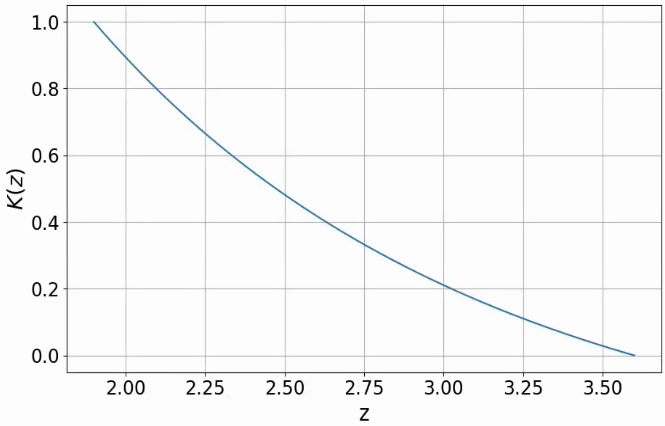
\includegraphics[scale=0.4]{kz}
%   \caption{Coefficient $K(z)$ défini dans l'équation~\ref{eq:lognormal_interp}.}
% \end{figure}


Les quasars sont ensuite tirés dans chaque voxel, avec une probabilité $P \propto \hat \delta_{\textsc{QSO}}$. Pour ce faire, nous générons une variable $\phi$ aléatoire uniforme entre 0 et 1 dans chaque voxel. Les voxels pour lesquelles $\phi < N(z) \hat \delta_{\textsc{QSO}}$ hébergent un quasar.
% Le facteur $N(z)$ est  un facteur de normalisation.
Le facteur $N(z)$ contient l'évolution avec le redshift du nombre de quasars par degré carré. Il contient aussi un facteur de normalisation.
\textbf{
  Une fois les quasars tirés, nous les plaçons aléatoirement dans leur voxel.
}
Puis, les quasars dont le redshift est en dehors de l'intervalle $[\num{1.8}\, ; \num{3.6}]$ sont écartés.
% Les quasars dont l'ascension droite est en dehors de l'inverval $[ - \Delta \alpha ; \Delta \alpha]$ et dont la déclinaison est en dehors de l'inverval $[ - \Delta \delta ; \Delta \delta]$ sont aussi écartés.
Les quasars dont l'ascension droite et la déclinaison sont en dehors des intervalles $[ - \Delta \alpha \, ; \Delta \alpha]$ et $[ - \Delta \delta \, ; \Delta \delta]$ sont aussi écartés.
L'ascension droite $\alpha$ et la déclinaison $\delta$ du point $(\textsc{x},\textsc{y},\textsc{z})$ sont données par
\begin{align}
  \label{eq:radec}
  \alpha &= \arctan(\frac{
  \cos(\alpha_0)\textsc{x} - \sin(\delta_0)\sin(\alpha_0)\textsc{y} + \cos(\delta_0)\sin(\alpha_0)\textsc{z}
  }{
  - \sin(\alpha_0)\textsc{x} - \sin(\delta_0)\cos(\alpha_0)\textsc{y} + \cos(\delta_0)\cos(\alpha_0)\textsc{z}
           }) \; ,\\
  \delta &= \arcsin(\frac{
           \cos(\delta_0)\textsc{y} + \sin(\delta_0) \textsc{z}
           }{
           \sqrt{\textsc{x}^2 + \textsc{y}^2 + \textsc{z}^2}
           }) \; .
\end{align}
Enfin, grâce au facteur $N(z)$, les quasars sont tirés selon la distribution en $z$ prédite pour DESI. Cette distribution est présentée sur la figure~\ref{fig:dndz_qso}. Cependant, nous tirons environ deux fois plus de quasars, afin de pouvoir simuler, entre autre, la sélection des cibles à l'aide du code \texttt{quickquasars} (présenté dans la section~\ref{sec:quickquasars}). De plus, cela permet d'utiliser les mocks pour d'autres projets, comme WEAVE\footnote{WEAVE est un spectrographe à fibre multi objet. Il possède \num{1000} fibres avec un champ de vue de $\SI{3.1}{\square\deg}$. Le relevé WEAVE-QSO prévoit d'observer \num{350000} quasars à grand redshift, sur un relevé de $\SI{6000}{\square\deg}$ \autocite{Pieri2016}.}, qui possèdent une densité de cible plus élevée que celle de DESI.
A la fin, nous obtenons environ \num{100} quasars à $z > \num{2.1}$ par degré carré.
\begin{figure}
  \centering
  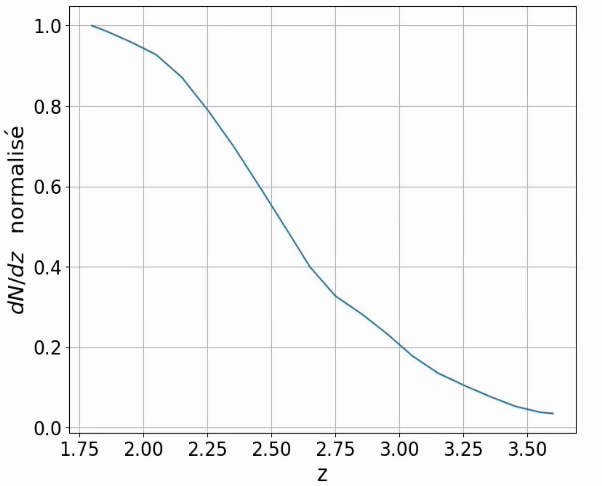
\includegraphics[scale=0.5]{dndz_qso}
  \caption{Distribution normalisée en redshift des quasars tirés dans les mocks.}
  \label{fig:dndz_qso}
\end{figure}

\paragraph{}
Une fois les quasars tirés, nous les déplaçons proportionnellement à leur vitesse $v_{\parallel}(z)$ le long de la ligne de visée.
La vitesse, à $z=0$, le long de la ligne de vitesse est obtenue comme
\begin{equation}
  \label{eq:vpar1}
  v_{\parallel} = \frac{v_{\textsc{x}} \textsc{x} + v_{\textsc{y}} \textsc{y} + v_{\textsc{z}} \textsc{z}}{\sqrt{\textsc{x}^2 + \textsc{y}^2 + \textsc{z}^2}} \; ,
\end{equation}
où les vitesses $v_{\textsc{x}}$, $v_{\textsc{y}}$ et $v_{\textsc{z}}$ sont les vitesses obtenus par transformation de Fourier inverse des vitesses $v_{k,\textsc{x}}$, $v_{k,\textsc{y}}$ et $v_{k,\textsc{z}}$, définies dans l'équation~\ref{eq:v2}.
Ainsi, un quasar situé à une distance $R$ sera replacé le long de la ligne de visée à une distance
\begin{equation}
  \label{eq:r_rsd}
 R \rightarrow  R + \frac{(1+z)}{H(z)} v_{\parallel}(z) \; ,  % (1+z) \frac{dG}{dz} \frac{1}{H_0 \frac{dG}{dz}(z=0)} v_{\parallel} \; ,
\end{equation}
où $v_{\parallel}(z)$ est relié à $v_{\parallel}$ à $z = 0$ par (voir équation~\ref{eq:v2})
\begin{equation}
  % v_{\parallel}(z) = (1+z) \frac{dG}{dz} \frac{H(z)}{H_0 \frac{dG}{dz}(z=0)} v_{\parallel} \; .
  % v_{\parallel}(z) = (1+z) \frac{H(z)}{H_0} \frac{1}{\frac{dG}{dz}(z=0)} \frac{dG}{dz} v_{\parallel} \; .
  % v_{\parallel}(z) =  \frac{H(z)}{H_0} \frac{dG/dz}{dG/dz(z=0)} v_{\parallel} \; .
  v_{\parallel}(z) = \frac{H(z) dG/dz}{[H(z) dG/dz]_{z=0}} v_{\parallel} \; .
\end{equation}
Le facteur $(1+z)$ dans l'équation~\ref{eq:r_rsd} vient de la conversion des distances en distances comobiles. Une fois tous les quasars déplacés, leur redshift est recalculé, puis ils sont stockés dans un catalogue. Pour chaque quasar, le catalogue contient leur position dans le ciel $(\alpha, \delta)$, leur redshift avec et sans RSD, ainsi qu'un identifiant unique.


\subsection{Création des lignes de visée}
\label{subsec:los_interp}
A cette étape, nous disposons d'un catalogue de quasars corrélés avec le champ de densité $\delta_{\mathrm{matière}}$ qui sera utilisé pour construire l'absorption \lya{}. Nous pouvons donc créer les lignes de visées à partir de chaque quasar et jusqu'à l'observateur, puis interpoler la boîte contenant le champ de densité le long de ces lignes de visée.
Dans un premier temps, nous commençons par définir le tableau en longueurs d'onde observées, sur lequel sera interpolé la boîte de densité. Nous choisissons une taille de pixel $d_{pix} = \SI{0.2}{\perh\Mpc}$. Les limites $\num{1.8} < z < \num{3.6}$ en redshift se traduisent par des limites $\num{3403.876} < \lambda < \SI{5592.082}{\angstrom}$ sur la longueur d'onde observée pour le \lya{}. Nous ajoutons la limite basse des spectrographes de DESI : $\lambda_{min} = \SI{3530}{\angstrom}$, que nous réduisons afin d'inclure certains métaux dans les forêts (cela sera expliqué dans la section~\ref{subsec:model_donnees}). Les longueurs d'onde observées couvrent donc $\num{3476.1877} < \lambda < \SI{5591.566}{\angstrom}$ à l'aide de \num{6524} pixels\footnote{Ces limites sont aussi choisies afin de garantir un nombre entier de pixels.}.

% Une fois ce tableau en longueur d'onde défini, nous le positionnons dans les boîtes afin de construire la ligne de visée à partir de chaque quasar.
% pour chaque quasar, nous calculons la position $(X,Y,Z)$ de chaque pixel.
% D'abord, le pixel $\lambda_{\textsc{QSO}} = (1+z_{\textsc{QSO}}) \lambda_{\mathrm{Ly}\alpha}$ est placé à la position $(\textsc{x}_{\textsc{QSO}}, \textsc{y}_{\textsc{QSO}}, \textsc{z}_{\textsc{QSO}})$ du quasar, et le vecteur est dirigé vers l'observateur.
Une fois ce tableau en longueur d'onde défini, nous faisons correspondre le pixel $\lambda_{\textsc{QSO}} = (1+z_{\textsc{QSO}}) \lambda_{\mathrm{Ly}\alpha}$ à la position $(\textsc{x}_{\textsc{QSO}}, \textsc{y}_{\textsc{QSO}}, \textsc{z}_{\textsc{QSO}})$ du quasar.
Puis, pour chaque pixel $i$ entre $\lambda_{min} = \num{3476.1877}$ et $\lambda_{\textsc{QSO}}$, la position $(\textsc{x}_i, \textsc{y}_i, \textsc{z}_i)$ du pixel est déterminée.
% La boîte est alors interpolé puis lissé.
% Une moyenne pondérée avec un lissage gaussien est alors appliquée à la boîte.
Pour chaque pixel, nous calculons une moyenne pondérée des voxels voisins avec un lissage gaussien.
  Ce lissage est nécessaire afin d'éviter le crénelage (\emph{aliasing}) aux petites échelles.
  Sans lissage, les spectres interpolés possèdent des discontinuitées (voir figure~\ref{fig:smoothing11}). Ces discontinuités rajoutent de la puissance parasite aux petites échelles lors du calcul du spectre de puissance.
  % Nous choisissons un lissage de largeur $\sigma = d_{cell}$.
  Nous appliquons donc un lissage gaussien, de largeur $\sigma = d_{cell}$.
% Pour chaque pixel, nous considérons les voxels appartenant au cube de 7 voxels de côté, centré sur le voxel dans lequel se trouve le pixel. Ce cube correspond à considérer les voxels compris à $\pm 3 \sigma$ du voxel central. %, avec $\sigma = d_{cell}$ (\#prov validé par le plot, demander à JM).
% Ceci représente donc, pour chaque pixel, une moyenne sur \num{343} voxels.
La figure~\ref{fig:smoothing11} présente le champ interpolé en considérant uniquement les voxels à $\pm 1 \sigma$. Trop peu de voxels sont considérés pour le calcul de chaque pixel, et le champ obtenu contient des discontinuités. La figure~\ref{fig:smoothing23} présente le champ interpolé en considérant les voxels à $\pm 2 \sigma$ (orange) et $\pm 3 \sigma$ (bleu). La différence entre les deux est faible, cependant certaines discontinuités subsistent pour le champ calculé avec $2 \sigma$, comme le montre le zoom sur le graphique de droite. Enfin, nous avons vérifié que les différences entre les champs obtenus avec $3$ et $4 \sigma$ sont plus faibles que $10^{-3}$, et donc négligeables par rapport au bruit dans chaque pixel. Nous nous limitons donc aux voxels compris à $\pm 3 \sigma$ du voxel central pour limiter le temps CPU.
\begin{figure}
  \centering
  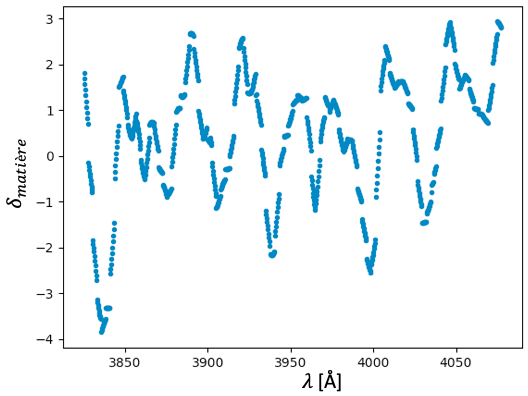
\includegraphics[scale=0.5]{smoothing11}
  \caption{Exemple de champ interpolé en utilisant les voxels à $\pm 1 \sigma$ du voxel central. Le champ ainsi interpolé possède de nombreuses discontinuitées. Ces discontinuitées produisent de la puissance supplémentaire aux petites échelles (effet de crénelage ou d'\emph{aliasing}).}
  \label{fig:smoothing11}
\end{figure}
\begin{figure}
  \centering
  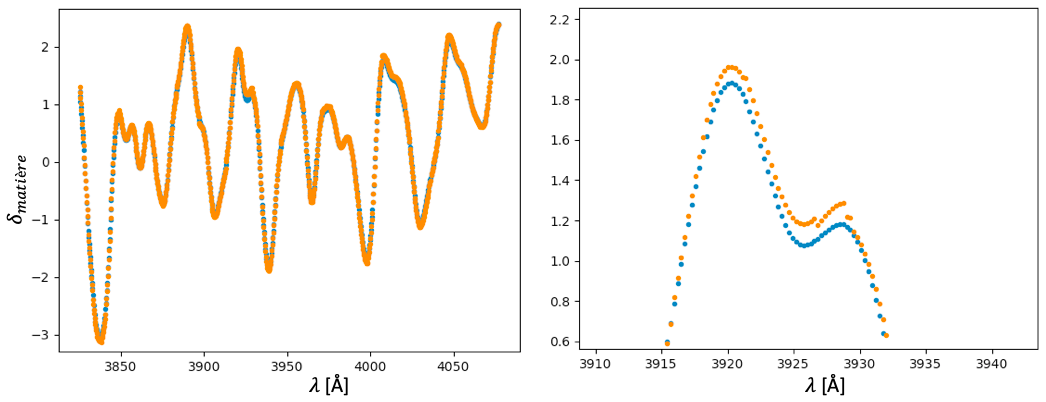
\includegraphics[scale=0.4]{smoothing23}
  \caption{Exemple de champ interpolé en utilisant les voxels à $\pm 2 \sigma$ (orange) et à $\pm 3 \sigma$ (bleu) du voxel central. Les discontinuitées sont beaucoup moins nombreuses que pour le champ interpolé avec $\pm 1 \sigma$ (figure~\ref{fig:smoothing11}). Cependant, certaines sont encore visibles sur le zoom, présenté sur le graphique de droite.}
  \label{fig:smoothing23}
\end{figure}
Pour chaque pixel, nous considérons les voxels appartenant au cube de 7 voxels de côté, centré sur le voxel dans lequel se trouve le pixel. % Ce cube correspond à considérer les voxels compris à $\pm 3 \sigma$ du voxel central. %, avec $\sigma = d_{cell}$ (\#prov validé par le plot, demander à JM).
Ceci représente donc, pour chaque pixel, une moyenne sur \num{343} voxels.
Le champ dans le pixel $i$ est alors donné par
% \begin{equation}
%   \delta_i = \sum_{j=0}^{342}  \frac{\delta(\vec r_j) \mathrm{e}^{\frac{-(\vec r_j - \vec r_i)^2 }{ \sigma_j^2}}}{\sigma_j^2} \; ,
% \end{equation}
% \#prov c'est pas correcte (voir le code)
\begin{equation}
  \delta_i = \frac{
    \sum\limits_{j=0}^{342} \delta_j w_{ij}
  }{
    \sum\limits_{j=0}^{342} w_{ij}
  } \; ,
\end{equation}
% (\#prov c'est pas beau les limites des sommes qui sont pas au dessus/en dessous)
avec
\begin{equation}
  w_{ij} = \exp(\frac{
    -(\vec r_j - \vec r_i)^2
  }{
    2 \sigma^2
  }) \; ,
\end{equation}
où $\vec r_j$ est la position du centre du voxel $j$, $\vec r_i$ celle du pixel $i$, et  $\delta_j$ est la valeur de la boîte au pixel $j$.
% , et enfin $\sigma^2 = d_{cell}^2$ est la largeur du lissage gaussien appliqué.

Ce calcul est effectué pour tous les pixels qui vérifient $\lambda_i < \lambda_{\textsc{QSO}}$, pour chaque quasar. Les boîtes interpolées sont la boîte $\delta_{\mathrm{matière}}$ utilisée pour construire l'absorption \lya{}, les trois boîtes de vitesse utilisées pour ajouter les RSD aux HCD tirés dans chaque ligne de visée (voir section~\ref{subsec:hcd}), et les six boîtes de gradient de vitesse afin d'ajouter les RSD au champ \lya{}.


\subsection{De la densité à l'absorption}
\label{subsec:density2absorption}
Une fois les lignes de visés interpolées, nous pouvons transformer le champ de densité en absorption \lya{}. Ceci est fait via la formule FGPA :
\begin{equation}
  \label{eq:fgpa2}
  % F = \exp( - a(z) \mathrm{e}^{b(z) G(z) \delta_{\mathrm{matière}}}) \;.
  F = \exp\left[ - a(z) \exp(b(z) G(z) \delta_{\mathrm{matière}})\right] \;.  
\end{equation}

\subsubsection{Les petites échelles}
La boîte $\delta_{\mathrm{matière}}$, utilisée dans l'équation~\ref{eq:fgpa2}, contient le champ de matière à grande échelle. Elle est construite grâce à la transformation de Fourier de la boîte $\delta_k$.
Ce champ est construit sur une grille d'intervalle $d_{cell} = \SI{2.19}{\perh\Mpc}$. Par conséquent, la plus petite échelle accessible est
\begin{equation}
  k_N = \frac{\pi}{d_{cell}} \sim \SI{1.43}{\h\per\Mpc} \; .
\end{equation}
Nous manquons donc toutes les fluctuations pour lesquelles $k > k_N$.
% Sans ces fluctuations le spectre de puissance à une dimension, défini comme
% \begin{equation}
%   \label{eq:p1d}
%   % P^{\mathrm{1D}}(\kpar{}) = \frac{1}{2 \pi} \int_{\kpar{}}^{\infty} k P(k) dk \; ,
%   P^{\mathrm{1D}}(\kpar{}) = \frac{1}{2 \pi} \int_{\kpar{}}^{\infty} \kperp{} P(\kpar{}, \kperp{}) d\kperp{} \; ,
% \end{equation}
% ne possède pas la bonne amplitude. De plus, ce sont ces fluctuations aux petites échelles qui contribuent principalement à la variance du champ. Le champ $F$ construit ne possède donc pas le bon niveau de bruit.
% \textbf{Ces fluctuations ne sont pas importante pour la corrélation à trois dimensions. En effet, nous calculons cette dernière pour mesurer l'échelle BAO, qui se situe à beaucoup plus grand échelle ($\sim \SI{100}{\perh\Mpc}$). De plus, comme expliqué dans la section~\ref{prov}, nous moyennons la fonction de corrélation à trois dimensions dans des bins de \SI{4}{\perh\Mpc} de large.
% }
Ces fluctuations ne sont pas importantes pour la corrélation à trois dimensions. La figure~\ref{fig:pk_smoothing} montre le spectre de puissance de la matière $P_{\mathrm{matière}}(k)$ à $z=0$ (noir), obtenu avec Camb, ainsi que l'effet du lissage gaussien et l'effet de la taille non nulle de ces voxels.
  La courbe bleu donne le spectre de puissance qui inclut l'effet du lissage gaussien. Il s'exprime comme
  \begin{equation}
    P(k) =  W^2(k) P_{\mathrm{matière}}(k) \; ,
  \end{equation}
  où $W(k)$ est le terme représentant le lissage gaussien appliqué à l'interpolation de la boîte $\delta_l$ :
  \begin{equation}
    \label{eq:gauss_smoothing}
    W(k) = \exp(- \frac{k^2 d_{cell}^2}{2}) \; .
  \end{equation}
  La courbe verte donne le spectre de puissance qui inclut l'effet de la taille des voxels. Celui-ci s'exprime comme
  \begin{equation}
    P(k) =   G^2(k) P_{\mathrm{matière}}(k) \; ,
  \end{equation}
  où $G(k)$ est le terme qui prend en compte la taille des voxels :
  \begin{equation}
    \label{eq:effet_reso}
    G(k) = \mathrm{sinc}\left(\frac{k d_{cell}}{2}\right)  \; .
  \end{equation}
  La courbe rouge donne le spectre de puissance qui inclut ces deux effets, c'est à dire multiplié par $W^2(k)G^2(k)$.
  La figure~\ref{fig:xi_smoothing} montre les fonctions de corrélation, qui sont les transformée de Fourier de ces spectres de puissance.
  % L'effet est faible (\#prov combien ?) et principalement localisé à petit $r$.
  Les effets liés au lissage gaussien et à la taille des voxels sont principalement localisés à petit $r$ et autour du pic BAO. Ces effets sont faibles, en particulier celui produit par la taille non nulle des voxels.
  Ainsi, ces fluctuations à petite échelle ne sont pas importantes pour la fonction de corrélation à trois dimension.

\begin{figure}
  \centering
  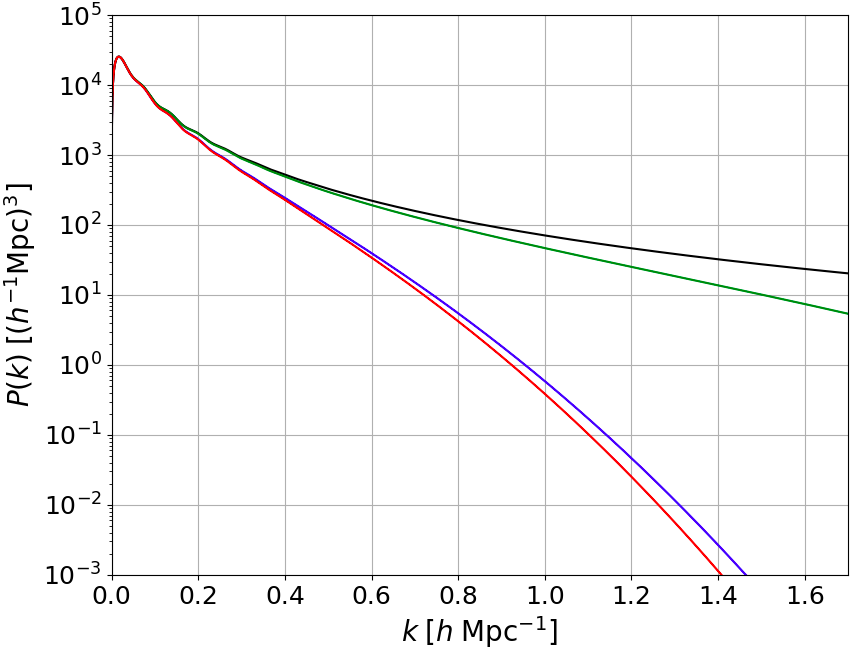
\includegraphics[scale=0.35]{pk_smoothing}
  \caption{Effet du lissage gaussien et de la taille non nulle des pixels sur le spectre de puissance. La courbe noire donne le spectre de puissance de la matière, obtenu avec Camb. La courbe bleu donne le spectre de puissance de la matière multiplié par $W^2(k)$ (équation~\ref{eq:gauss_smoothing}). La courbe verte donne le spectre de puissance multiplié par $G^2(k)$ (équation~\ref{eq:gauss_smoothing}). Enfin la courbe rouge donne le spectre de puissance multiplié par $W^2(k) G^2(k)$.}
  \label{fig:pk_smoothing}
\end{figure}
\begin{figure}
  \centering
  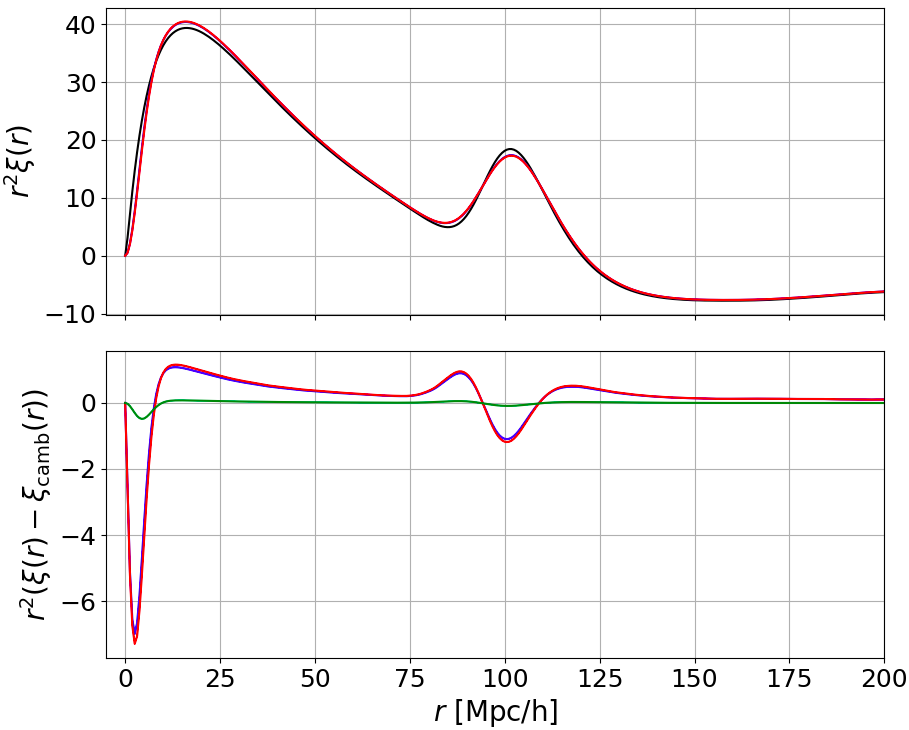
\includegraphics[scale=0.38]{xi_smoothing}
  \caption{Effet du lissage gaussien et de la taille non nulle des pixels sur la fonction de corrélation des mocks. Le graphique du haut montre les fonctions de corrélation obtenues à partir du spectre de puissance de Camb (noir), du spectre de puissance de Camb multiplié par $W^2(k)$ en bleu, du spectre de puissance de Camb multiplié par $G^2(k)$ en vert, et du spectre de puissance de Camb multiplié par $W^2(k)G^2(k)$ en rouge (voir équations~\ref{eq:gauss_smoothing} et~\ref{eq:effet_reso}). Le graphique du bas montre la différence entre les courbes bleue et noire, en bleu, entre les courbes vert et noire, en vert, ainsi qu'entre les courbes rouge et noire, en rouge.}
  \label{fig:xi_smoothing}
\end{figure}
\begin{figure}
  \centering
  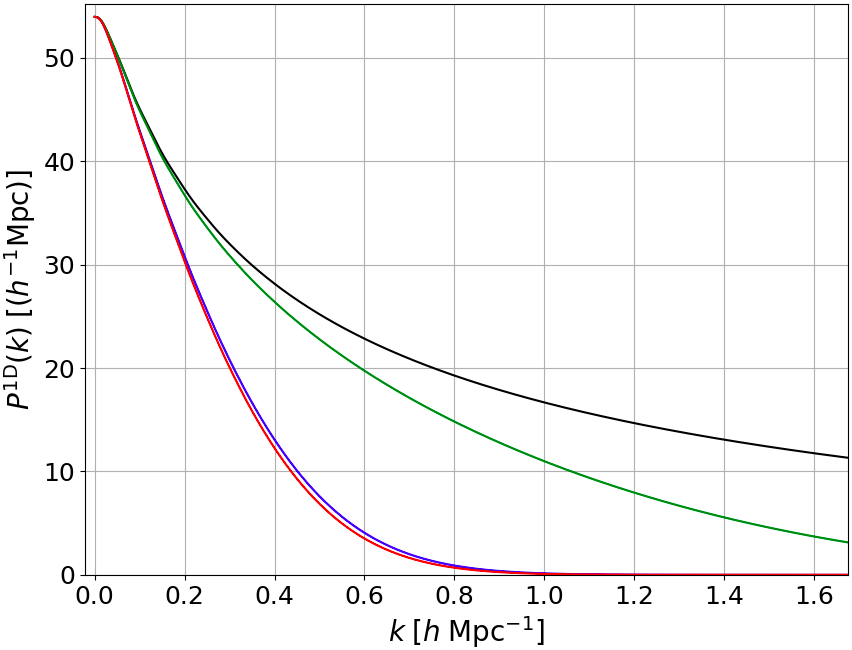
\includegraphics[scale=0.35]{p1d_smoothing}
  \caption{Effet du lissage gaussien et de la taille non nulle des pixels sur le spectre de puissance à une dimension. La courbe noire donne le spectre de puissance à une dimension obtenu à partir du spectre de puissance de la matière (équation~\ref{eq:p1d}). La courbe bleu donne $P^{\mathrm{1D}}$ obtenu à partir du spectre de puissance de la matière multiplié par $W^2(k)$ (équation~\ref{eq:gauss_smoothing}). La courbe verte donne $P^{\mathrm{1D}}$ obtenu à partir du spectre de puissance  de la matière multiplié par $G^2(k)$ (équation~\ref{eq:gauss_smoothing}). Enfin la courbe rouge donne $P^{\mathrm{1D}}$ obtenu à partir du spectre de puissance de la matière multiplié par $W^2(k) G^2(k)$.
  L'effet dominant sur le spectre de puissance à une dimension est l'effet du lissage gaussien.}
  \label{fig:p1d_smoothing}
\end{figure}

\textbf{Cependant, ces fluctuations sont importantes pour le spectre de puissance à une dimension. Celui-ci est calculé en corrélant les pixels d'une même forêt. Il donne la puissance mesurée le long de la ligne de visée. Pour un mode $\kpar{}$ donné, on peut montrer que le spectre de puissance à une dimension est donné par l'intégrale du spectre de puissance à trois dimensions sur la direction transverse à la ligne de visée \autocite{lumsden_clustering_1989} :}
\begin{equation}
  \label{eq:p1d}
  P^{\mathrm{1D}}(\kpar{}) = \frac{1}{2 \pi} \int_{0}^{\infty} \kperp{} P(\kpar{}, \kperp{}) d\kperp{} \; .
\end{equation}
\textbf{Les spectres des quasars sondent la densité le long de la ligne de visée, avec une résolution transverse extrèmement faible, équivalente à la taille d'un quasar (inférieure au parsec). Le calcul du spectre de puissance sur ces spectres implique donc une intégrale jusqu'à $\kperp{} = \infty$.
% Avec la taille non nulle des voxels, l'intégrale s'effectue seulement jusqu'à $k_N$. De plus, le lissage gaussien appliqué à l'interpolation de la boîte $\delta_l$ réduit davantage l'amplitude de ce spectre de puissance. Ces deux effets sont représentés sur la figure~\ref{prov} (\#prov faire la figure). Contrairement au cas à trois dimensions, l'effet de la taille des voxels et du lissage gaussien est important pour le spectre de puissance à une dimension.
% En effet, ce spectre de puissance le long d'une ligne de visée est beaucoup plus sensible au bruit que le spectre de puissance calculé sur une colonne de section de $(\SI{2.19}{\perh\Mpc})^2$.
% A cause de ces deux effets, l'amplitude du spectre de puissance à une dimension n'est pas correcte. Et ainsi, la variance du champ, donnée par l'intégrale du $P^{\mathrm{1D}}$, n'est pas correcte non plus.
  Dans notre cas, le spectre de puissance à trois dimensions $P(\kpar{}, \kperp{})$ à intégrer est le spectre de puissance de la matière $P_{\mathrm{matière}}(\kpar{}, \kperp{})$ multiplié par $G^2(\kpar{}, \kperp{})W^2(\kpar{}, \kperp{})$.
  L'effet de $G^2$ et $W^2$ sur $P^{\mathrm{1D}}$ est présenté sur la figure~\ref{fig:p1d_smoothing}.
  Contrairement au cas de la fonction de corrélation à trois dimensions, l'effet de la taille des voxels et du lissage gaussien est important pour le spectre de puissance à une dimension : les termes $G^2$ et $W^2$ réduisent l'amplitude des modes aux petites échelles, qui ont une contribution importante pour tous les $\kpar{}$ lors du calcul de l'intégrale de l'équation~\ref{eq:p1d}.
% Autrement dit, le spectre de puissance le long d'une ligne de visée est beaucoup plus sensible aux petites échelles que le spectre de puissance calculé sur une colonne de section de $(\SI{2.19}{\perh\Mpc})^2$, car dans le cas de ce dernier, les fluctuations liées aux modes perpendiculaires à la colonne et plus petits que $k = \pi / \SI{2.19}{\h\per\Mpc}$ sont moyennées. Ces fluctuations ne sont donc pas importantes dans ce cas là, mais le sont pour le spectre de puissance à une dimension. Lorsque les fluctuations aux petites échelles sont manquantes, l'amplitude du spectre de puissance à une dimension n'est pas correcte, et la variance du champ, donnée par l'intégrale de $P^{\mathrm{1D}}$, n'est pas correcte non plus.
% En effet, le spectre de puissance le long d'une ligne de visée est beaucoup plus sensible aux petites échelles (grands $k$) que le spectre de puissance calculée sur une colonne de section $(\SI{2.19}{\perh\Mpc})^2$ : les termes $G^2$ et $W^2$ réduisent l'amplitude des modes aux petites échelles, qui sont importants 
% Sans les fluctuations à petite échelle, l'amplitude du spectre de puissance à une dimension n'est pas correcte. Et ainsi, la variance du champ, donnée par l'intégrale du $P^{\mathrm{1D}}$, n'est pas correcte non plus.
% Lorsque ce spectre de puissance est calculé dans des voxels
Pour palier ce problème, nous rajoutons indépendamment sur chaque ligne de visée un champ $\delta_s$ (\emph{small scales} : petites échelles) au champ $\delta_{\mathrm{matière}}$ que nous appelons désormais $\delta_{l}$ (\emph{large scales} : grandes échelles) :}
\begin{equation}
  \label{eq:fgpa3}
  % F = \exp( - a(z) \mathrm{e}^{b(z) G(z) (\delta_l + \delta_s)}) ;.
  F = \exp\left[ - a(z) \exp(b(z) G(z) (\delta_l + \delta_s))\right] ;.
\end{equation}
Comme ce champ n'est pas corrélé d'une ligne de visée à une autre, il ne participe pas à la fonction de corrélation à trois dimensions\footnote{Lors du calcul de la fonction de corrélation à trois dimensions, nous ne considérons pas les paires de pixels issues de la même forêt (voir section~\ref{subsec:cf_estimateur})}.
% Afin d'ajouter la bonne quantité de fluctuations aux petites échelles, pour chaque ligne de visée nous générons un GRF à une dimension $\delta_{k,s}$, d'une taille supérieure à celle de la forêt pour éviter les corrélations d'une extrémité à l'autre.
Afin d'ajouter la bonne quantité de fluctuations aux petites échelles, pour chaque ligne de visée nous générons un GRF à une dimension $\delta_{k,s}$.
Puis, nous multiplions ce champ par
\begin{equation}
  \sqrt{\frac{P_{s}(k,z_{\mathrm{eff}})}{d_{pix}}} \; ,
\end{equation}
où $z_{\mathrm{eff}}$ est le redshift moyen de la forêt, et $P_{s}$ est le spectre de puissance qu'il faut appliquer à $\delta_{k,s}$ afin que $\delta_F$ possède le bon $P^{\mathrm{1D}}$. $\delta_{k,s}$ est créé avec une taille supérieure à celle de la forêt, pour éviter les corrélations d'une extrémité à l'autre. La détermination de $P_{s}$ est détaillée dans la section~\ref{sec:tuning}. Puis, nous obtenons $\delta_s$ à l'aide de la transformation de Fourier inverse de $\delta_{k,s}$.
  Avant d'ajouter $\delta_s$ à $\delta_l$, nous corrigeons la dépendance en $z$ de chacun des $\delta_s$ de la forêt. En effet, $\delta_s$ est construit de façon à obtenir le bon spectre de puissance à une dimension au redshift moyen de la forêt. Les pixels situés en bord de forêt n'auront donc pas le bon $P^{\mathrm{1D}}$. Ainsi, nous corrigeons chaque $\delta_s$ comme :
  \begin{equation}
    \delta_s(z) \rightarrow \delta_s(z) \frac{\sigma_s(z)}{\sigma_s(z_{\mathrm{eff}})} \; ,
  \end{equation}
  où $\sigma_s$ est l'écart type du champ $\delta_s$. Celui-ci est relié au spectre de puissance $P_{s}$ par :
  \begin{equation}
    \label{eq:sigma_s}
    \sigma_s = \frac{1}{d_{pix}N} \left( P_{s}(0) + P_{s}(k_{Ny}) + 2 \sum_{j=1}^{\frac{N}{2} - 1}P_{s}\left(\frac{2 \pi}{d_{pix}N} j\right)\right) \; ,
  \end{equation}
  où $k_{Ny} = \pi / d_{pix} \sim \SI{15.7}{\perh\Mpc}$ est le mode de Nyquist : c'est le mode maximal accessible pour une taille de pixel donnée.


\subsubsection{Les RSD}
\label{subsubsec:rsdlya}
% Une fois les petites échelles ajoutées, nous obtenons un champ d'absorption $F$ qui possède le bon spectre de puissance à 3 dimension pour les échelles $k_N < k < k_{max}$, avec
% \begin{equation}
%   \label{eq:kny}
%   k_{max} = \frac{2 \pi}{1536 d_{cell}} \sim \SI{1.9e-3}{\h\per\Mpc} \; ,
% \end{equation}
% (\#prov y a un facteur 2 en trop pour kny?)
% ainsi que le bon spectre de puissance à une dimension.
Une fois les petites échelles ajoutées, nous obtenons un champ d'absorption $F$ qui possède le bon spectre de puissance à trois dimensions, ainsi que le bon spectre de puissance à une dimension.
Cependant, le champ d'absorption $F$ ne possède pas de RSD pour l'instant, car il est construit à partir du spectre de puissance $P_{\mathrm{matière}}(k)$ qui est isotrope.
Initiallement, nous pensions ajouter les RSD au niveau du spectre de puissance : multiplier le GRF intial $\delta_k$ par $(1 + \beta \mu^2)P_{\mathrm{matière}}(k, \mu)$, avec $\mu = k_z / k$.
Mais cette solution n'est pas envisageable car les lignes de visées ne sont pas parallèles (elles l'étaient pour les mocks précédents, développés pour BOSS), et nous ne pouvons donc pas confondre l'axe $k_z$ avec l'axe de la ligne de visée $\kpar{}$.
Une autre solution est d'utiliser le champ de vitesse défini dans l'équation~\ref{eq:v1}. Chaque pixel d'absorption est alors déplacé proportionnellement à la vitesse particulière du gaz dans la cellule considérée. Puis l'absorption est modifiée en fonction de la différence des vitesses des pixels voisins. En effet, si cette différence est non nulle, le gaz se retrouve comprimé par endroit, et détendu dans d'autres, modifiant l'absorption dans chaque pixel.
Cette méthode pour ajouter les RSD dans les mocks \lya{} est la méthode choisie par \textcite{LeGoff2011} et \textcite{Farr2019}.
Ce n'est pas la solution que nous utilisons ici. Afin d'inclure les RSD dans le champ d'absorption $F$, nous utilisons le champ de gradient de vitesse $\eta_{\parallel}$, présenté dans la section~\ref{subsubsec:vitesses}.
Contrairement à la méthode qui utilise le champ de vitesse, la solution qui ajoute le champ $\eta_{\parallel}$ au champ $\delta_l$ permet de prédire la fonction de corrélation des mocks. Nous décrivons cette prédiction dans la section suivante.
% Cependant, du fait que les lignes de visées ne sont pas parrallèles (elles l'étaient pour les mocks précédents, développés pour BOSS), nous ne pouvons pas confondre l'axe $k_z$ avec l'axe de la ligne de visée $\kpar{}$.
% \textbf{Une autre solution est d'utiliser le champ de vitesse}
% Nous avons alors choisi d'utilisé le champ de gradient de vitesse $\eta_{\parallel}$, présenté dans la section~\ref{subsubsec:vitesses}.


Plusieurs essais ont été menés afin de savoir comment inclure correctement le champ $\eta_{\parallel}$ dans FGPA.
La première solution envisagée était de modifier la profondeur optique $\tau$. Comme $\delta_{\tau} = \tau / \overline \tau - 1$ est conservée lors du passage dans l'espace des redshifts, nous modifiions $\tau$ (équation~\ref{eq:fgpa1}) comme
\begin{equation}
  \tau \rightarrow \tau + \overline \tau \eta_{\parallel} \; .
\end{equation}
Cette solution produisait une trop faible quantité de RSD. Nous avons alors décidé d'inclure les RSD causées par les petites échelles. Similairement à $\delta_l$ et $\delta_s$, nous ajoutions à la profondeur optique la contribution aux grandes et petites échelles $\eta_l$ et $\eta_s$. En faisant ceci, nous étions plus proche de ce que nous aurions obtenu avec une taille de voxel plus petite.
La profondeur optique était alors donnée par
% à la profondeur optique, car c'est ce que nous aurions obtenu avec une taille de voxel plus petite. La profondeur optique était alors donnée par
\begin{equation}
  \tau = a \exp\left[b G (\delta_l + \delta_s)\right] + \overline \tau (\eta_l + \eta_s) \; .
\end{equation}
Cette solution produisait la bonnne quantité de RSD. Cependant, la profondeur optique était négative pour un nombre non négligeable de pixels, résultant en une absorption $F > 1$ non physique pour ces pixels.
Finalement, nous avons décidé d'inclure le gradient de vitesse directement au niveau du champ $\delta$.
% Nous présentons dans les lignes qui suivent la solution retenue.
Le champ $\eta_{\parallel}$ est donc ajouté, en plus du champ $\delta_s$, au champ $\delta_l$. Ceci nous permet de retrouver la formule de Kaiser (équation~\ref{eq:kaiser5}). De plus, cette solution ne produit pas de pixel avec $F > 1$.
Afin de gérer la bonne quantité de RSD, nous ajoutons un coefficient $c$, qui dépend de $z$. L'ajustement de ce paramètre nous permet d'obtenir la bonne dépendance en $z$ pour $\beta_{\mathrm{Ly}\alpha}$. La formule FGPA devient donc
\begin{equation}
  \label{eq:fgpa4}
  F = \exp\left[ - a(z) \exp(b(z) G(z) (\delta_l + \delta_s + c(z)\eta_{\parallel}))\right] ;.  
\end{equation}
Les champs $\delta_l$, $\delta_s$ et $\eta_{\parallel}$ sont calculés à $z=0$. De plus, le facteur $f$ que nous avons laissé de côté dans la section~\ref{subsubsec:vitesses} n'est pas explicité ici : pour les redshifts $z > 2$, l'univers est dominé par la matière et donc, en bonne approximation, nous avons $f(z) \sim 1$. Les paramètres $a(z)$, $b(z)$, $c(z)$, ainsi que $P_{s}(k,z)$ sont ajustés afin d'obtenir les bons $b_{\mathrm{Ly}\alpha}(z)$, $\beta_{\mathrm{Ly}\alpha}(z)$, $\overline F(z)$ et $P^{\mathrm{1D}}_{\mathrm{Ly}\alpha}(k,z)$. L'ajustement est décrit dans la section~\ref{sec:tuning}.


\paragraph{}
\textbf{
  % Les différentes étapes relatives à la création des forêts de chaque quasar sont résumées sur la figure~\ref{fig:building_trans}. De haut en bas, les graphiques de cette figure représentent : le champ à grande échelle $\delta_l$, la somme $\delta_l + c(z)\eta_{\parallel}$, le champ $\delta_g$ défini comme $\delta_g = \delta_l + \delta_s + c(z) \eta_{\parallel}$, la fraction de flux transmise $F$, et enfin le spectre du quasar. Cette dernière étape est produite par le code \texttt{quickquasars} (voir section~\ref{sec:quickquasars}). Un DLA avec une grande densité de colonne est visible à $\lambda_{\mathrm{RF}} \sim \SI{1165}{\angstrom}$.
  Les différentes étapes relatives à la création des forêts de chaque quasar sont résumées sur la figure~\ref{fig:building_trans}. De haut en bas, le premier graphique de cette figure présente les champs à grande échelle $\delta_l$, $c(z)\eta_{\parallel}$ et la somme des deux. Le deuxième présente la somme $\delta_l + \delta_s$ et le champ $\delta_g$ défini comme $\delta_g = \delta_l + \delta_s + c(z) \eta_{\parallel}$. Le troisième présente la fraction de flux transmise $F$, et enfin le dernier graphique présente le spectre du quasar. Cette dernière étape est produite par le code \texttt{quickquasars} (voir section~\ref{sec:quickquasars}). Un DLA avec une grande densité de colonne est visible à $\lambda_{\mathrm{RF}} \sim \SI{1165}{\angstrom}$. La remontée obersée pour les longueurs d'onde proches de \SI{1200}{\angstrom} est causée par la proximité de la raie \lya{}.
}
  

\begin{figure}
  \centering
  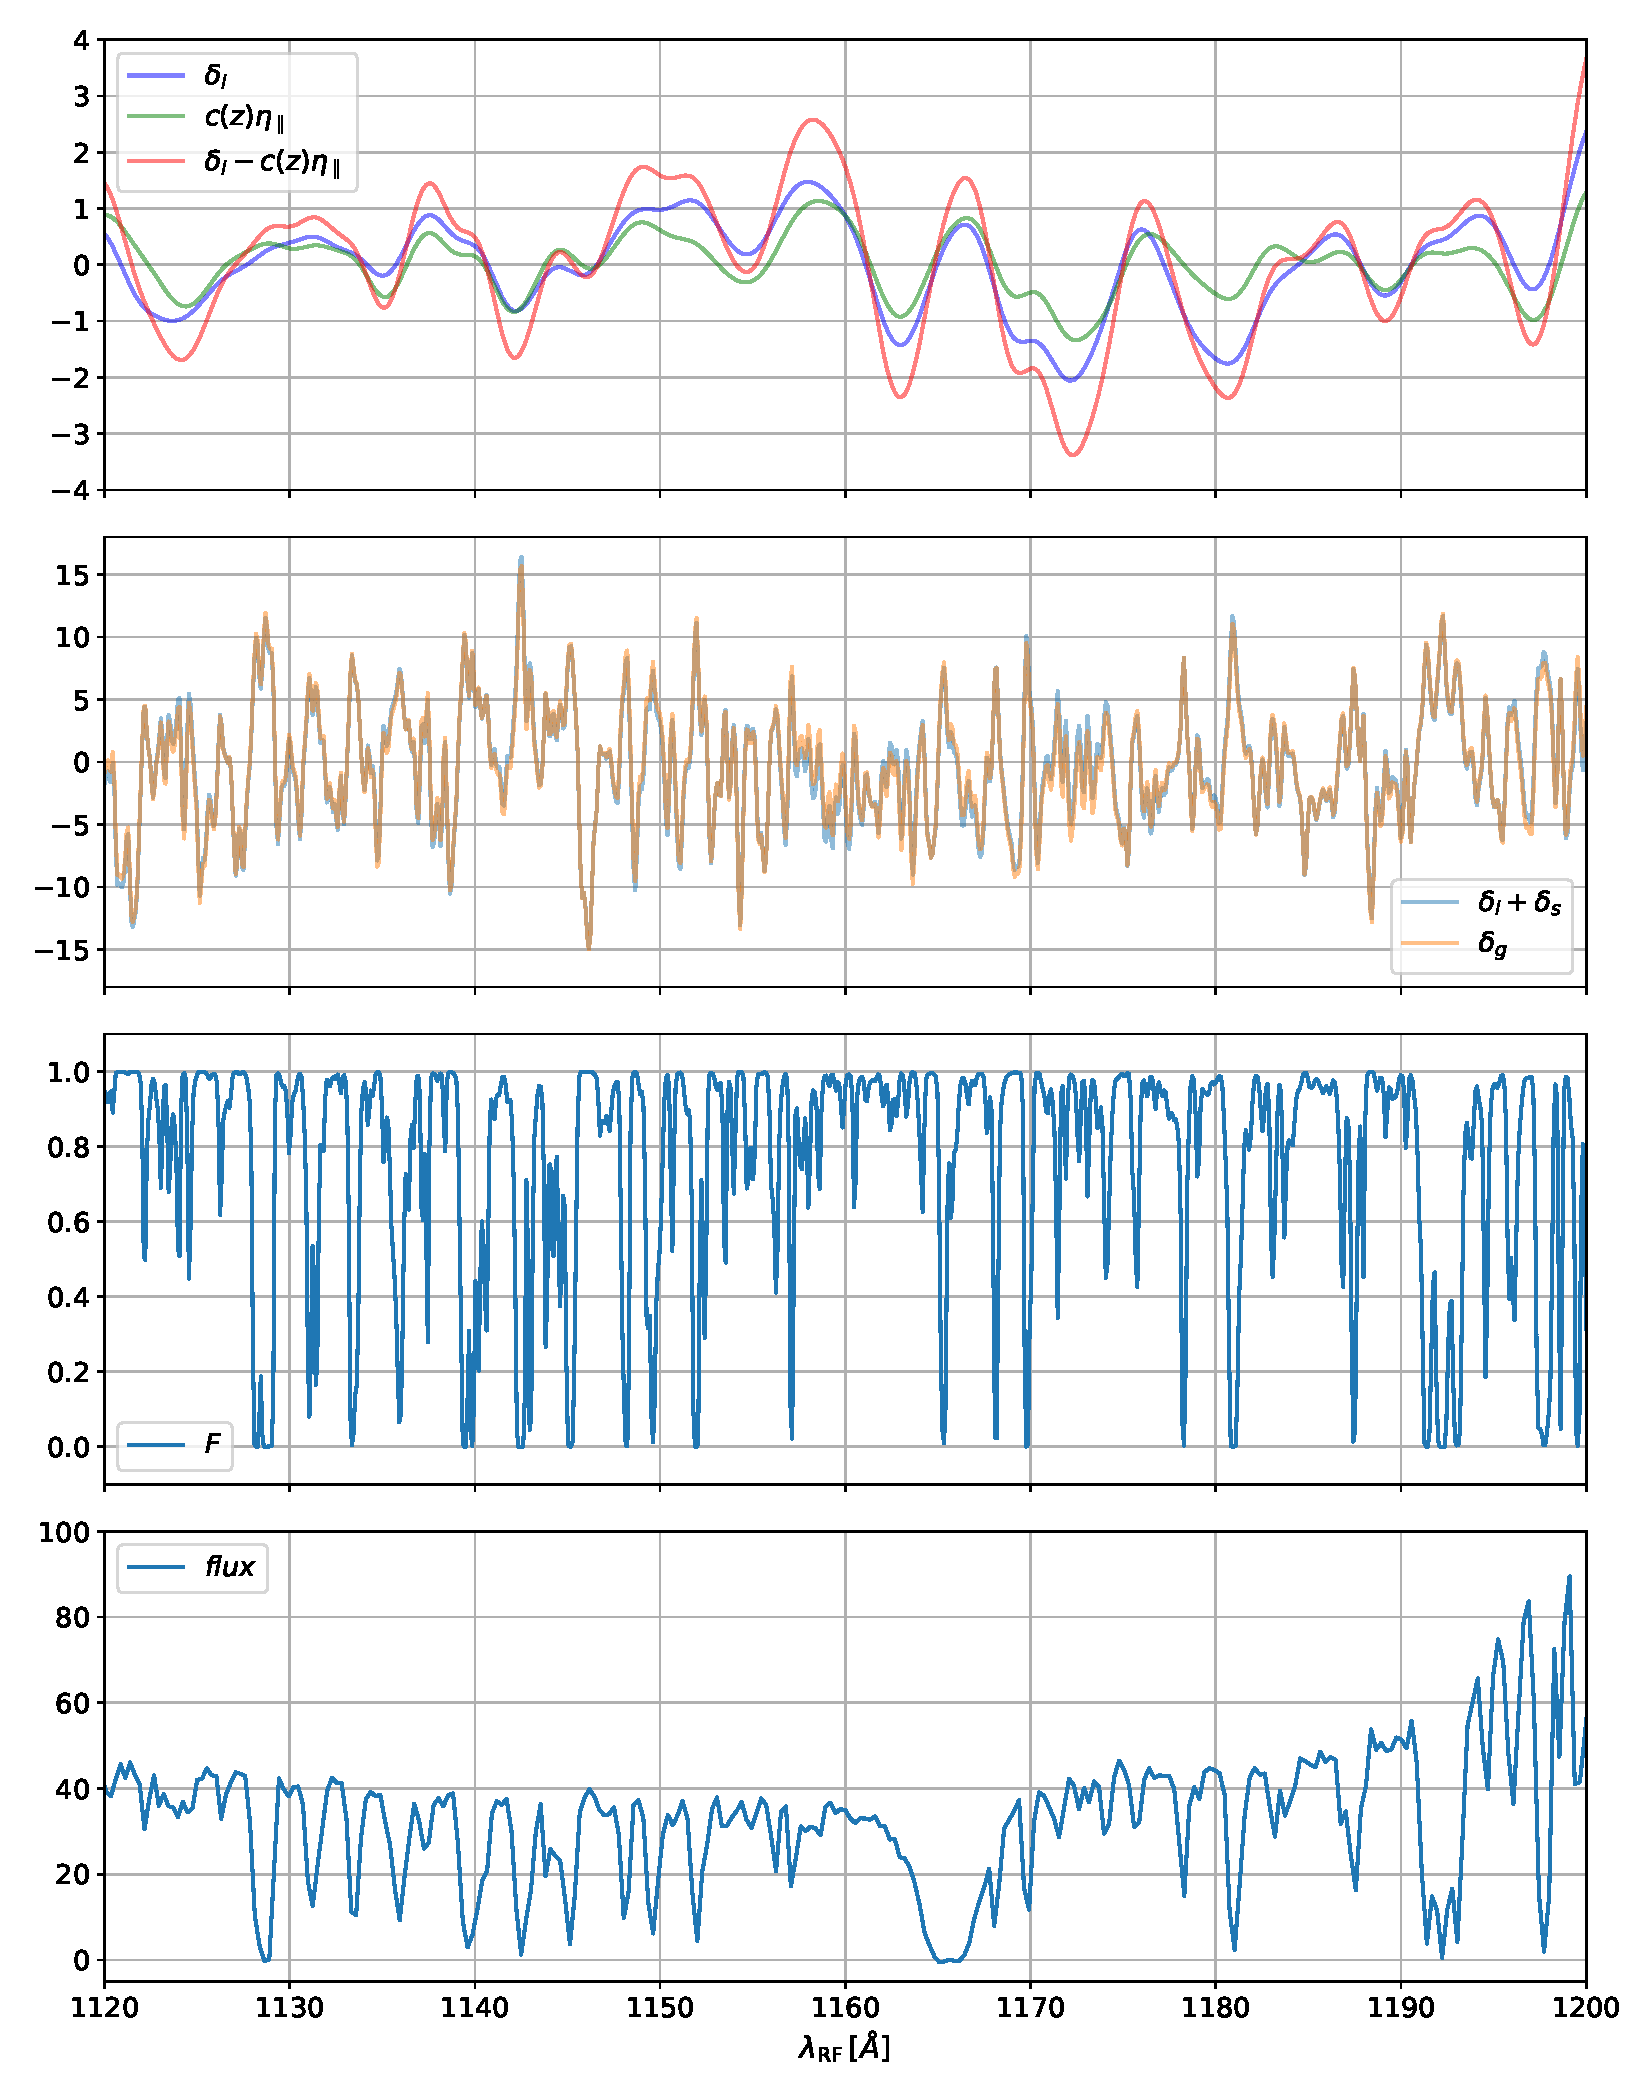
\includegraphics[scale=0.6]{building_trans.pdf}
  \caption{
    % De haut en bas : le champ à grande échelle $\delta_l$, la somme $\delta_l + c(z)\eta_{\parallel}$, le champ $\delta_g$ défini comme $\delta_g = \delta_l + \delta_s + c(z) \eta_{\parallel}$, la fraction de flux transmise $F$, et enfin le spectre du quasar. Le quasar est situé à un redshift $z=\num{3.167}$. La raie \lyb{} est visible à gauche dans le graphique du bas, et la base du pic \lya{} est visible à droite. Une DLA avec une grande densité de colonne est aussi visible à $\lambda_{\mathrm{RF}} \sim \SI{1165}{\angstrom}$.
    De haut en bas, le premier graphique présente les champs à grande échelle $\delta_l$, $c(z)\eta_{\parallel}$ et la somme des deux. Le deuxième présente la somme $\delta_l + \delta_s$ et le champ $\delta_g$ défini comme $\delta_g = \delta_l + \delta_s + c(z) \eta_{\parallel}$. Le troisième présente la fraction de flux transmise $F$, et enfin le dernier graphique présente le spectre du quasar. Un DLA avec une grande densité de colonne est visible à $\lambda_{\mathrm{RF}} \sim \SI{1165}{\angstrom}$.
  }
  \label{fig:building_trans}
\end{figure}


\subsubsection{La prédiction}
\label{subsubsec:pred}

% Il aurait été possible d'implémenter les RSD différemment. Une solution serait, par exemple, de déplacer chaque pixel d'absorption proportionnellement à la vitesse particulière du gaz dans la cellule considéré, puis de modifier l'absorption en fonction du gradient de vitesse dans cette cellule. En effet, si le gradient de vitesse est non nul, le gaz se retrouve comprimé par endroit, et détendu dans d'autres, modifiant l'absorption dans chaque cellule. Cette méthode pour ajouter les RSD dans des mocks \lya{} est la méthode choisie par \textcite{le_goff_simulations_2011} et \textcite{Farr2019}.
% Ce n'est pas la méthode que nous choisissons ici, car celle-ci ne permet pas de prédire la fonction de corrélation obtenue avec les mocks. Dans le cas où $F$ est relié au GRF $\delta$ par une fonction analytique (équation~\ref{eq:fgpa4}), il est possible de relier la fonction de corrélation $\xi_F$ du champ $F$ à la fonction de corrélation $\xi_g$ du champ $\delta$ \autocite{Font-Ribera2012}. Ces deux fonctions de corrélations sont reliées par la relation
% La méthode que nous utilisons, décrite dans la section précédente, a l'avantage d'avoir une fonction de corrélation prédictible. C'est pour cela que nous avons fait le choix de cette méthode.
La méthode que nous utilisons pour ajouter les RSD, décrite dans la section précédente, a l'avantage d'avoir une fonction de corrélation prédictible. % C'est pour cela que nous avons fait le choix de cette méthode.
Dans les lignes qui suivent, nous expliquons comment calculer la prédiction de la fonction de corrélation. Comme décrit par \textcite{Font-Ribera2012}, dans le cas où le champ $\delta_F$ est une fonction d'un champ gaussien $\delta_g$, il est possible de relier la fonction de correlation $\xi_F$ du champ $\delta_F$ à la fonction de corrélation $\xi_g$ du champ $\delta_g$. La fonction de corrélation $\xi_F(r_{12})$ pour la séparation $r_{12}$ est reliée à $\xi_g(r_{12})$ par
\begin{equation}
  \label{eq:xig2xif}
  \xi_F(r_{12}) = \int_{- \infty}^{\infty} d\delta_{g1} \int_{- \infty}^{\infty} d\delta_{g2}
  \frac{
    \exp\left[-
      \frac{
        \delta_{g1}^2 + \delta_{g2}^2 - 2 \delta_{g1} \delta_{g2} \xi_g(r_{12})
      }{
        2 ( 1 - \xi_g^2(r_{12})))
      }\right]
  }{
    2 \pi \sqrt{1 - \xi_g^2(r_{12})}
  }
  \delta_F(\delta_{g1})\delta_F(\delta_{g2})
  \; ,
\end{equation}
où $\delta_g$ est un GRF de variance $1$ et $\delta_F$ est le champ d'absorption calculé à partir du champ gaussien.
% , et $r_{12}$ est la distance qui sépare les deux points où sont évalués les champs $\delta_g$ et $\delta_F$.
Dans notre cas, le champ $\delta_g$ représente le champ $\delta_l + \delta_s + c(z)\eta_{\parallel}$. Ce champ est un champ gaussien, de valeur moyenne nulle et de variance $\sigma_g^2$. Cette variance est dominé par la variance de $\delta_s$.
Nous compensons le fait que $\sigma_g^2 \neq 1$ en remplaçant $\xi_g$ par $\xi_g / \sigma_g^2$ dans l'équation~\ref{eq:xig2xif}. % Ainsi, grâce à l'équation~\ref{eq:xig2xif}, pour chaque valeur de $\xi_g \in [-1 ; 1]$, nous pouvons déterminer $\xi_F$.
Dans cette équation, $\xi_F(r_{12})$ ne dépend que de la valeur de $\xi_g(r_{12})/ \sigma_g^2$. Nous construisons donc une table qui permet de relier chaque valeur de $\xi_g/ \sigma_g^2 \in [-1 \, ; 1]$ à la valeur $\xi_F$ correspondante.
\begin{figure}
  \centering
  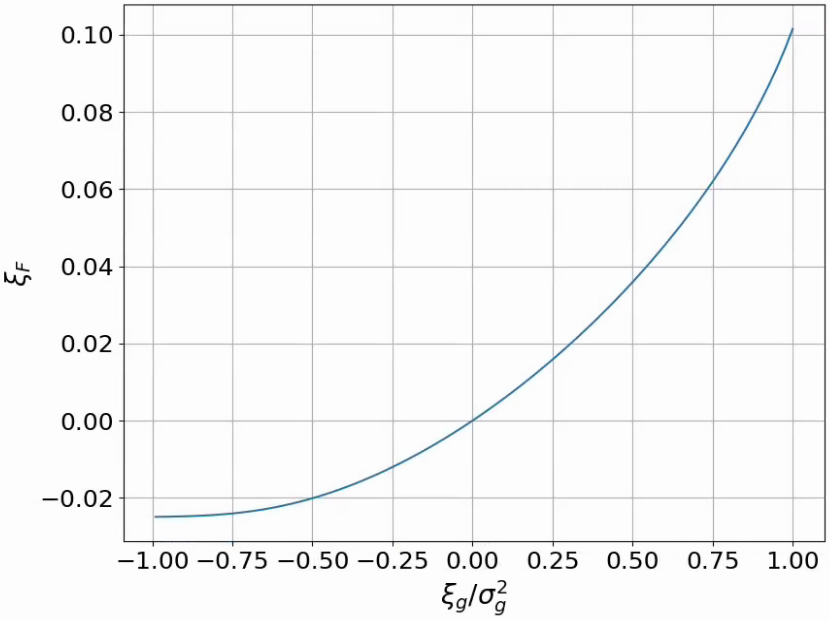
\includegraphics[scale=0.4]{xiF_vs_xig}
  \caption{La fonction de corrélation $\xi_F$ obtenue à l'aide de l'équation~\ref{eq:xig2xif} pour chaque valeur de $\xi_g/ \sigma_g^2 \in [-1 \, ; 1]$.}
  \label{fig:xiF_vs_xig}
\end{figure}
La figure~\ref{fig:xiF_vs_xig} montre la fonction de corrélation $\xi_F$ obtenue, en fonction de $\xi_g/ \sigma_g^2$.
% Afin d'obtenir la prédiction pour $\xi(r, \mu)$, nous utilisons les formules décrites dans \textcite{hamilton_measuring_1992} :
% Afin d'obtenir la prédiction dans l'espace des redshifts, nous commençons par relier $\xi_g(r, \mu)$ à la fonction de corrélation $\xi(r)$ que suit le champ $\delta_l$ :
% De plus, nous pouvons relier la fonction de corrélation dans l'espace des redshifts $\xi_g(r, \mu)$, à la fonction de corrélation $\xi(r)$ que suit le champ $\delta_l$ :
% Par ailleurs, puisque $\delta_s$ ne participe pas à la fonction de corrélation à trois dimension du champ $\delta_g$, nous relions la fonction de corrélation dans l'espace de sredshift $\xi_g(r, \mu)$, à la fonction de corrélation $\xi(r)$ que suit le champ $\delta_l$ :
Par ailleurs, puisque $\delta_s$ n'est pas corrélé d'une forêt à une autre, il ne participe pas au spectre de puissance à trois dimensions.
D'après la formule de Kaiser (équation~\ref{eq:kaiser5}), le champ $\delta_g$ suit le spectre de puissance
\begin{equation}
  \label{eq:pk_g}
    P_g(k) = (1 + c \mu_k^2)^2 P_l(k) \; ,
  \end{equation}
  où $P_l$ est le spectre de puissance que suit le champ $\delta_l$.
  La figure~\ref{fig:xi_g} montre la fonction de corrélation du champ $\delta_g$ mesuré dans les mocks ainsi que la fonction de corrélation obtenue à partir du spectre de puissance de l'équation~\ref{eq:pk_g} (voir le passage de $P_g(k)$ à $\xi_g(r,\mu)$ dans les lignes qui suivent). Nous vérifions que ces deux fonctions de corrélation sont en accord.
\textbf{  Nous observons cependant de petites différences essentiellement le long de la ligne de visée.
  Cela pourrait être dû à l'effet de la taille des voxels utilisés pour construire les boîtes de gradient de vitesse $\eta$, ou possiblement au lissage gaussien appliqué à $\eta_{\parallel}$.}
  \begin{figure}
    \centering
    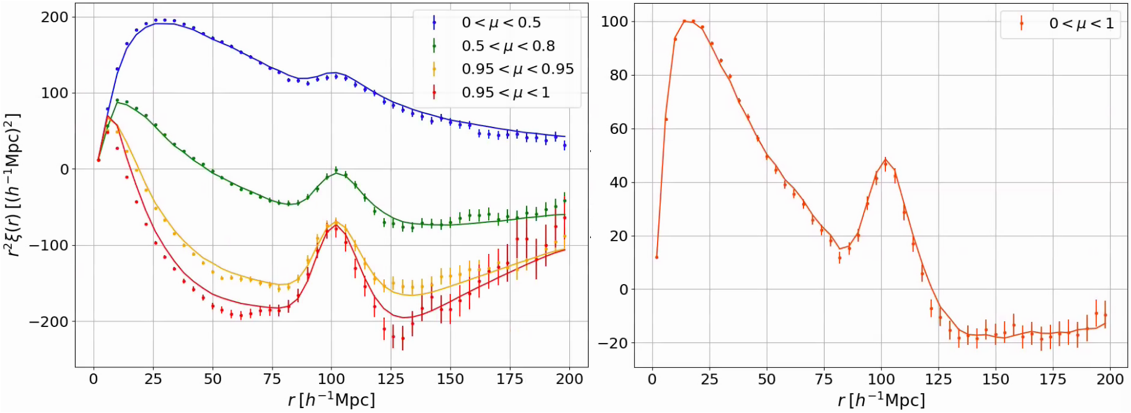
\includegraphics[scale=0.4]{xi_g}
    \caption{Fonctions de corrélation du champ $\delta_g$ (points) et prédiction de cette fonction de corrélation (équations~\ref{eq:pk_g} et~\ref{eq:hamilton1}. Le graphique de gauche montre les corrélations dans quatre bins en $\mu$. Celui de droite montre les corrélations dans la gamme $0 < \mu < 1$. La corrélation mesurée sur le champ $\delta_g$ est en bon accord avec la corrélation prédite, même s'il existe un écart le long de la ligne de visée.}
    \label{fig:xi_g}
  \end{figure}

  Afin de relier la fonction de corrélation dans l'espace des redshifts $\xi_g(r, \mu)$ que suit le champ $\delta_g$ à la fonction de corrélation $\xi(r)$ que suit le champ $\delta_l$, nous utilisons les formules données dans \textcite{Hamilton1992} :
\begin{equation}
  \label{eq:hamilton1}
  % \xi(r, \mu) = \xi_0(r) + \frac{1}{2}\left(3 \mu^2 - 1\right) \xi_2(r) + \frac{1}{8}\left(35 \mu^4 - 30 \mu^2 + 3\right) \xi_4(r) \; ,
  \xi_g(r, \mu) = \xi_0(r) +  P_2(\mu) \xi_2(r) +  P_4(\mu) \xi_4(r) \; ,
\end{equation}
avec
\begin{align}
  \label{eq:hamilton2}
  \xi_0(r) &= \left(1 + \frac{2}{3} c + \frac{1}{5} c^2\right) \xi(r) \; , \\
  \xi_2(r) &= \left(\frac{4}{3} c + \frac{4}{7} c^2\right) \left[\xi(r) - \overline \xi(r)\right] \; , \\
  \xi_4(r) &= \frac{8}{35} c^2\left[\xi(r) + \frac{5}{2} \overline \xi(r) - \frac{7}{2} \overline{\overline \xi}(r)\right] \; ,
\end{align}
et
\begin{align}
  \label{eq:hamilton3}
  \overline \xi(r) = 3 r^{-3} \int_0^r \xi(s) s^2 ds \; , \\
  \overline{\overline \xi}(r) = 5 r^{-5} \int_0^r \xi(s) s^4 ds \; .
\end{align}
Les $P_l(\mu)$ sont les polynômes de Legendre :
\begin{equation}
  P_0(\mu) = 1 \hspace{0.2cm} ; \hspace{0.8cm} P_2(\mu) = \frac{1}{2} (3 \mu^2 - 1) \hspace{0.2cm} ; \hspace{0.8cm}   P_4(\mu) = \frac{1}{8} (35 \mu^4 - 30 \mu^2 + 3) \; .
\end{equation}
% et $\beta$ est le paramètre RSD du \lya{}.
% Ces équations sont tirés de la publication de \textcite{Hamilton1992}.
Afin d'obtenir la prédiction $\xi_F^{pred}(r, \mu)$, nous commençons par calculer  le spectre de puissance que suit la boîte $\delta_l$ :
\begin{equation}
  P(k) = W^2(k)P_{\mathrm{matière}}(z=0) \; ,
\end{equation}
où $W(k)$ est le terme représentant le lissage gaussien appliqué à l'interpolation de la boîte $\delta_l$ (équation~\ref{eq:gauss_smoothing}).
% \begin{equation}
%   \label{eq:gauss_smoothing}
%   % W(k) = \mathrm{e}^{- \frac{k^2 d_{cell}^2}{2}} \;.
%   W(k) = \exp(- \frac{k^2 d_{cell}^2}{2}) \;.
% \end{equation}
% \# prov Expliquer pourquoi on ne prend pas en compte le terme lié à la résolution de la boîte ? Regarder si l'effet est négligeable
Nous négligeons ici l'effet de la taille non nulle des voxels sur le spectre de puissance (équation~\ref{eq:effet_reso}).
% Cet effet peut être modélisé en multipliant le spectre de puissance précédent par $G^2(k)$, où $G(k)$ s'exprime comme
% \begin{equation}
%   \label{eq:effet_reso}
%   G(k) = \mathrm{sinc}\left(\frac{k d_{cell}}{2}\right) \;.
% \end{equation}
La figure~\ref{fig:xi_smoothing} montre l'effet de $W(k)$ et $G(k)$ sur la fonction de corrélation. L'effet lié à $G(k)$ est nettement moins important que celui lié à $W(k)$.
% (\#prov il y a pas un facteur $\frac{1}{2}$ en trop ? on a $\sigma_{smooth}^2 = 2 d_{cell}^2$)
Puis, à l'aide d'une transformation de Fourier du spectre de puissance, nous obtenons la fonction de corrélation $\xi(r)$ que suit le champ $\delta_l$ obtenu par interpolation avec lissage des boîtes.
% Nous définissons le champ $\delta_g$ comme
% \begin{equation}
%   \delta_g = G(z)(\delta_l + \delta_c + c(z)\eta_{\parallel}) \; .
% \end{equation}
Nous calculons ensuite la fonction de corrélation dans l'espace des redshifts $\xi_g(r, \mu)$ que suit le champ $\delta_g$ gràce à l'équation~\ref{eq:hamilton1}. La figure~\ref{fig:xi_g} présente cette fonction de corrélation mesurée sur une réalisation. Enfin, pour tous les couples $(r,\mu)$ nécessaires, nous obtenons la fonction de corrélation $\xi_F(r, \mu)$ du champ $\delta_F$ comme la valeur correspondante à la valeur tabulée $\xi_g(r, \mu) / \sigma_g^2$ pour $\xi_g$.



\subsection{Ajout des HCD}
\label{subsec:hcd}
Les HCD ont un effet important sur les fonctions de corrélation, nous simulons donc aussi leur présence. De manière à avoir une corrélation entre les HCD et les autres traceurs des mocks, nous utilisons la boîte de densité $\delta_l$ pour tirer les HCD. Nous ne considérons pas la somme $\delta_l + \delta_s$ car les HCD sont des surdensités qui se situent dans les structures à grandes échelles : une résolution de \SI{2.19}{\perh\Mpc} est suffisante. De plus, l'ajout de $\delta_s$ bruiterait la corrélation entre les HCD et les autres traceurs. En effet, l'écart type $\sigma_s$ du champ $\delta_s$ est entre 4 et 6 fois plus important que celui du champ $\delta_l$, et L'écart type $\sigma_g$ est dominé à plus de \SI{95}{\percent} par $\sigma_s$. Du fait que $\delta_s$ ne possède pas de corrélation à 3 dimensions, les HCD se situeraient principalement dans des pics de bruit non corrélés.

% Nous commençons donc avec le champ de densité $\delta_l$ interpolé le long de la ligne de visée. Pour chaque ligne de visée,
Contrairement aux quasars, les HCD sont tirés selon les pics du champ $\delta_l$ : nous identifions les pixels dans lesquelles $\delta_l$ est au dessus d'un certain seuil, puis les HCD sont tirés dans ces pixels selon une loi de Poisson.
Le seuil $\nu$ est défini en fonction du biais souhaité pour les HCD.
L'appendice A de \textcite{Font-Ribera2012a} relie le rapport $b_{\nu} / b_g$ au seuil $\nu$ :
\begin{equation}
  \label{eq:biais_seuil}
  \left(\frac{b_{\nu}}{b_g}\right)^2 = \frac{p_g(\nu)}{\left( \int_{\nu}^{\infty} d\delta_g p_g(\delta_g) \right)^2} \int_{\nu}^{\infty} dy_1 p_g(y_1) y_1 \; ,
\end{equation}
où $b_{\nu}$ est le biais obtenu avec le seuil $\nu$, $b_g$ est le biais du champ gaussien, et $p_g$ donne la densité de probabilité du champ gaussien de variance 1. Dans notre cas, $b_g = 1$.
% , et $\nu$ est défini comme
% \begin{equation}
%   \nu = \int_{\nu}^{\infty} d\delta_g p_g(\delta_g) \; .
% \end{equation}
% Nous pouvons remarquer que l'intégrale au numérateur de l'équation~\ref{eq:biais_seuil} donne la densité probabilité du champ gaussien $p_g(\nu)$ évaluée au seuil $\nu$.
% L'équation~\ref{eq:biais_seuil} est donc équivalente à
% \begin{equation}
%  b_{\nu} = \frac{p_g(\nu)}{\int_{\nu}^{\infty} d\delta_g p_g(\delta_g)} \; .
% \end{equation}
En utilisant le changement de variable $u = y_1^2 / 2$, l'intégrale au dénominateur de l'équation~\ref{eq:biais_seuil} vaut simplement $p_g(\nu)$ :
\begin{equation}
  \label{eq:biais_seuil2}
  \int_{\nu}^\infty dy_1 p_g(y_1)y_1 = 
\int_{\nu}^\infty dy_1 \frac{\exp(-y_1^2/2)}{\sqrt{2\pi}}  y_1 = \int_{\nu^2/2}^\infty du \frac{\exp(-u)}{\sqrt{2\pi}}=\frac{\exp(-\nu^2/2)}{\sqrt{2\pi}}=p_g(\nu) \; .
\end{equation}
L'équation~\ref{eq:biais_seuil} est donc équivalente à
\begin{equation}
 b_{\nu} = \frac{p_g(\nu)}{\int_{\nu}^{\infty} d\delta_g p_g(\delta_g)} \; .
\end{equation}
% old
% Pour un seuil $\nu$, le biais obtenu est donné par (\#prov ref Font + expliquer, cf mail JM)
% \begin{equation}
%   b_{\nu} = \frac{pdf(\nu)}{cdf(-\nu)} \; ,
% \end{equation}
% où $pdf(\nu)$ donne la densité de probabilité de $\nu$, et $cdf(-\nu)$ est la fonction de répartition : la probabilité d'être au dessus du seuil $\nu$. % Ainsi, pour avoir un biais de 2, il faut que la probabilité que le champ prenne la valeur $\nu$ soit 2 fois plus grande que la probabilité que le champ soit au dessus du seuil $\nu$.
% Afin d'obtenir le seuil pour un biais donné, nous calculons $b_{\nu}$ pour une large gamme de seuils $\nu$ puis nous interpolons $b_{\nu}$ sur $\nu$.
% Ainsi, pour un biais $b$, nous connaissons le seuil $\nu(b)$ à choisir.
Afin d'obtenir le seuil pour un biais donné, nous tabulons $b_{\nu}$ pour une large gamme de seuils $\nu$, puis nous interpolons  $\nu$ en fonction de $b_{\nu}$.
  Le graphique de gauche de la figure~\ref{fig:bnu_lambda} montre le biais $b_{\nu}$ en fonction du seuil $\nu$.
\begin{figure}
  \centering
  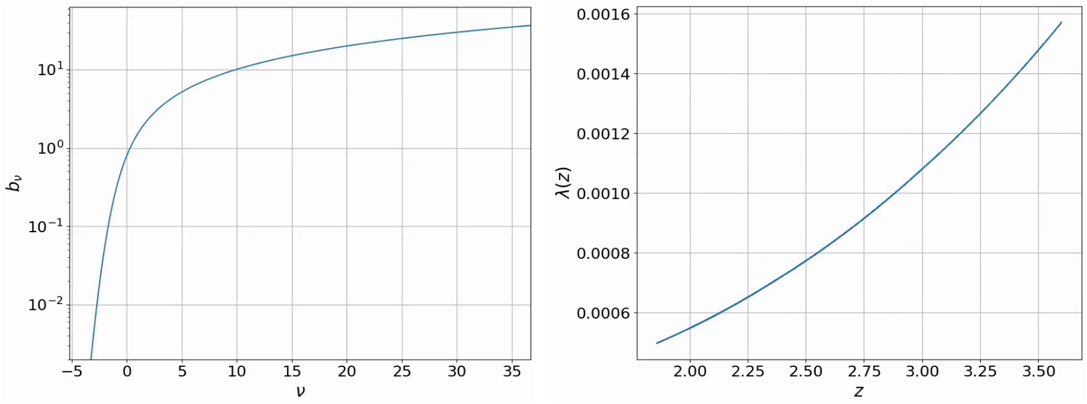
\includegraphics[scale=0.42]{bnu_lambda}
  \caption{Le graphique de gauche montre le biais $b_{\nu}$ obtenu pour un seuil $\nu$. Le graphique de droite montre le paramètre $\lambda(z)$, utilisé pour tirer les HCD.}
  \label{fig:bnu_lambda}
\end{figure}
Dans notre cas, le champ $\delta_l$ suit une distribution de probabilité gaussienne. Cependant, sa variance n'est pas égale à 1. De plus, le champ $\delta_l$ interpolé le long des lignes de visée correspond au champ de matière à $z=0$. Ainsi, pour obtenir un biais $b_{\textsc{HCD}}$, pour chaque redshift nous  calculons le seuil $\nu$ comme si nous visions un biais $b = b_{\textsc{HCD}} \sigma_l G(z)$. Le terme $\sigma_l$ prend en compte la variance du champ $\delta_l$, et $G(z)$ le fait que $\delta_l$ soit construit à $z=0$. Nous choisissons de tirer les HCD avec un biais $b_{\textsc{HCD}} = 2$.
Une fois les pixels pouvant héberger un HCD identifiées, nous tirons dans chacune d'entre elles les HCD avec une loi de poisson de paramètre
\begin{equation}
  \lambda(z) = \frac{N(z)}{cdf(-\nu(z))} \; ,
\end{equation}
où $N(z)$ donne le nombre moyen de HCD attendu par pixel et $\nu(z)$ le seuil au redshift $z$. Le nombre de HCD attendu est donné par la librairie \texttt{pyigm}\footnote{https://github.com/pyigm}. La distribution en redshift des HCD est présentée sur le graphique de gauche de la figure~\ref{fig:distrib_dla}, et le paramètre $\lambda(z)$ sur le graphique de droite de la figure~\ref{fig:bnu_lambda}. En pratique, du fait que $\lambda(z) \ll 1$, il est très rare d'avoir plus d'un HCD par pixel\footnote{Lorsqu'un pixel contient plusieurs HCD, ces HCD sont gardés et une densité de colonne leur est assignée. Ces deux HCD sont alors ajoutés au spectre synthétique par \texttt{quickquasars} (voir section~\ref{sec:quickquasars}), ce qui résulte en un seul HCD avec une densité de colonne valant la somme des densités de colonne des deux HCD tirés dans le pixel.}.
Une fois tous les HCD tirés, nous leur assignons une densité de colonne dans la gamme $\num{17.2} < \log(n_{\textsc{HI}}) < \num{22.5}$, selon la distribution donnée par \texttt{pyigm}. Cette distribution est présentée sur le graphique de droite de la figure~\ref{fig:distrib_dla}.
\begin{figure}
  \centering
  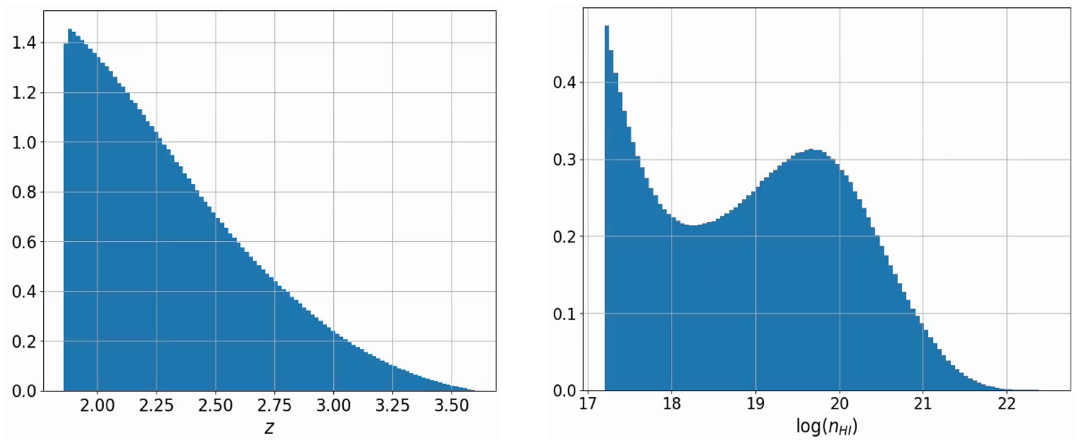
\includegraphics[scale=0.38]{distrib_dla}
  \caption{Gauche : distribution normalisée en redshift des HCD. Droite : distribution normalisée de $\log(n_{\textsc{HI}})$ des HCD. Ces distributions proviennent de la librairie \texttt{pyigm}.}
  \label{fig:distrib_dla}
\end{figure}
Enfin, nous ajoutons les RSD aux HCD tirés. Chaque HCD tiré est déplacé le long de la ligne de visée proportionnellement à la vitesse $v_{\parallel}(z)$. Comme pour les quasars, la vitesse le long de la ligne de visée à $z=0$ est donnée par
\begin{equation}
v_{\parallel} = \frac{v_{\textsc{x}} \textsc{x} + v_{\textsc{y}} \textsc{y} + v_{\textsc{z}} \textsc{z}}{\sqrt{\textsc{x}^2 + \textsc{y}^2 + \textsc{z}^2}} \; .
\end{equation}
% où $v_{\textsc{x}}$, $v_{\textsc{y}}$ et $v_{\textsc{z}}$ sont les boîtes de vitesse interpolées le long de la ligne de visée.
où, cette fois ci, $v_{\textsc{x}}$, $v_{\textsc{y}}$ et $v_{\textsc{z}}$ sont les vitesses le long de la ligne de visée provenant de l'interpolation des boîtes de vitesse (voir section~\ref{subsec:los_interp}).
Ainsi, un HCD à un redshift $z$ sera déplacé à un redshift
\begin{equation}
  % z \rightarrow  z + (1+z) H(z) \frac{dG}{dz} \frac{1}{H_0 \frac{dG}{dz}(z=0)} v_{\parallel} \; .
  z \rightarrow  z + \frac{(1+z)}{c} \frac{H(z) dG/dz}{[H(z) dG/dz]_{z=0}} v_{\parallel} \; .
\end{equation}
Dans les mocks que nous décrivons ici, le profil d'absorption des HCD n'est pas ajouté dans les forêts. Nous produisons uniquement un catalogue qui regroupe tous les HCD tirés. Le profil d'absorption est ajouté au spectre de chaque quasar par le code \texttt{quickquasars}, qui utilise le catalogue de HCD que nous produisons.


\section{Production des mocks}
Comme expliqué au début de ce chapitre, l'objectif des mocks est de reproduire les données d'eBOSS et de DESI. Etant donné que le relevé d'eBOSS est contenu dans le relevé de DESI, nous simulons directement le relevé DESI. Ainsi, lorsque nous avons besoin de simuler le relevé d'eBOSS, nous retirons les quasars qui ne sont pas contenu dans ce relevé.
\begin{figure}
  \centering
  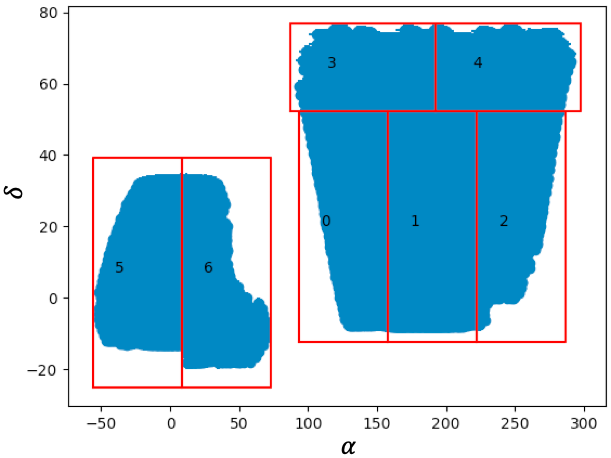
\includegraphics[scale=0.5]{chunks}
  \caption{Découpage du relevé de DESI en 7 chunks.}
  \label{fig:chunks}
\end{figure}
% La taille des boîtes choisie ($\num{2560}\times\num{2560}\times\num{1536}$ voxels) et leur résolution (\SI{2.19}{\perh\Mpc}) ne suffisent pas à couvrir les \num{14000} degrés carrés de DESI. Pour palier ce problème, nous construisons sept \emph{chunks} indépendants, que nous assemblons pour former le relevé de DESI. Le découpage du relevé en sept chunks est montré sur la figure~\ref{fig:chunks}.
% Ce choix d'assembler sept boîtes de densité plutôt que d'en utiliser une seule a été contraint par la mémoire maximale des n{\oe}uds.
Les mocks ont été produits au centre de calcul NERSC\footnote{National Energy Research Scientific Computing Center (NERSC), a U.S. Department of Energy Office of Science User Facility operated under Contract No. DE-AC02-05CH11231.}, avec la machine Cori.
% Sur cette machine, nous avons utilisé les n{\oe}uds ``Haswell''.
% Ces n{\oe}uds possèdent $\num{128}\,\mathrm{Go}$ de mémoire vive. De manière à créer nos boîtes de densité, via la transformation de Fourier à trois dimensions, il faut, pour chaque boîte, que l'intégralité de son contenu soit accessible depuis un même endroit.
% Nous pourrions distribuer la mémoire et effectuer la transformation de Fourier sur plusieurs n{\oe}uds à l'aide de la librairie MPI.
% Cependant nous n'avions pas l'expertise nécessaire. Nous effectuons donc les transformations de Fourier sur un seul n{\oe}ud, ce qui explique le découpage du relevé en sept chunks indépendants.
% Nous profitons néanmoins des \num{32} c{\oe}urs par n{\oe}ud pour paralléliser notre code. Chaque c{\oe}ur possède 2 hyper-threads, ce qui permet de gérer 64 tâches simultanément sur un même n{\oe}ud.
% \#prov taille des boites : \num{37.5} Go (box) + \num{37.5}/2 Go (boxk) + \num{37.5}/2 Go (k) : 75 Go. On est loin des 128 Go.
Sur cette machine, nous avons utilisé les n{\oe}uds ``Haswell''.
Ces n{\oe}uds possèdent $\num{128}\,\mathrm{Go}$ de mémoire vive. De manière à créer nos boîtes de densité, via la transformation de Fourier à trois dimensions, il faut, pour chaque boîte, que l'intégralité de son contenu soit accessible depuis un même endroit.
Nous pourrions distribuer la mémoire et effectuer la transformation de Fourier sur plusieurs n{\oe}uds à l'aide de la librairie MPI.
Cependant nous n'avions pas l'expertise nécessaire. Nous effectuons donc les transformations de Fourier sur un seul n{\oe}ud.
Nous profitons néanmoins des \num{32} c{\oe}urs par n{\oe}ud pour paralléliser notre code. Chaque c{\oe}ur possède 2 hyper-threads, ce qui permet de gérer 64 tâches simultanément sur un même n{\oe}ud.
Lors de la construction des boîtes (voir section~\ref{subsec:densityfields}), nous avons besoin de stocker en mémoire la boîte dans l'espace réel, la boîte dans l'espace $k$, et la boîte contenant la norme de $k$, cette dernière étant utilisée pour construire les boîtes de vitesses et de gradients de vitesse (équations~\ref{eq:v2} et~\ref{eq:eta1}).
Etant donné la mémoire disponible sur chaque n{\oe}ud, les boîtes ne doivent pas dépasser $\num{42}\,\mathrm{Go}$. Cette mémoire disponible et la taille des voxels choisie (\SI{2.19}{\perh\Mpc}) ne permettent pas de générer l'entièreté du relevé DESI avec une seule boîte.
Nous choisissons donc de découper le relevé en sept chunks indépendants, chacun étant généré par une boîte de $\num{2560}\times\num{2560}\times\num{1536}$ voxels. Chacune des boîtes représente un volume de $\num{37.5}\,\mathrm{Go}$. A la fin de la production, ces sept chunks sont assemblés pour reconstruire le relevé de DESI. Le découpage du relevé en sept chunks est montré sur la figure~\ref{fig:chunks}.
Dans les lignes qui suivent, nous détaillons les différents éléments du code.
Le schéma~\ref{fig:schema_prod} résume la situation.
\begin{figure}
  \centering
  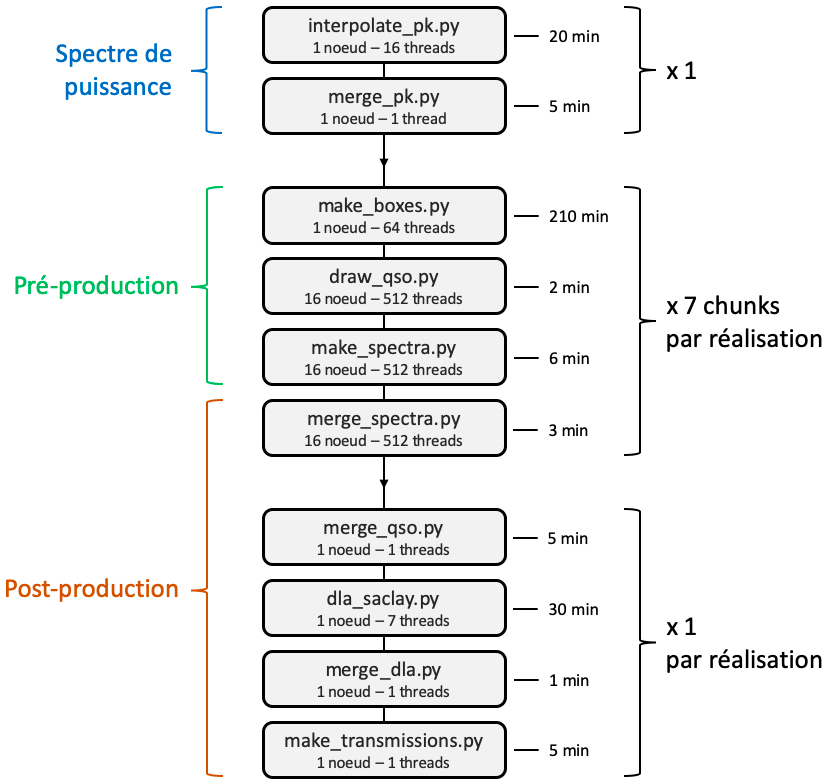
\includegraphics[scale=0.55]{schema_prod}
  \caption{Schéma illustratif du fonctionnement des mocks. Le premier bloc (bleu) génère le spectre de puissance nécessaire à la création des boîtes. Puis, pour chaque chunk de chaque réalisation, la pré-production (vert) génère les boîtes, tire les quasars, et interpole les lignes de visée. Enfin, la post-production (orange) rassemble les morceaux de lignes de visée et construit les forêts \lya{} pour chaque chunk. Puis, elle regroupe le résultat de chaque chunk, construit les catalogues finaux de quasars et HCD et produit les fichiers transmissions pour chaque réalisation. Chaque case indique le nom du code, ainsi que les conditions dans lesquelles il est tourné. Les temps d'exécution indiqués sont approximatifs.}
  \label{fig:schema_prod}
\end{figure}
Le première module, \texttt{interpolate\_pk.py} permet de calculer puis d'interpoler les quatres spectres de puissance $P_{\textsc{QSO},i}$ et $P_{\mathrm{matière}}$ sur la grille $\num{2560}\times\num{2560}\times\num{1536}$ dans l'espace k. Le code est lancé séparément sur 16 morceaux de la boîte, puis le code \texttt{merge\_pk.py} permet de rassembler des 16 morceaux des spectres de puissance interpolés et de les sauver au format FITS (Flexible Image Transport System). Cette étape est effectuée une seule fois, car les spectres de puissance sont communs à toutes les réalisations. Le module suivant est \texttt{make\_boxes.py}.
% Ce code lit les spectres de puissance interpolés puis construit les différentes boîtes de densité, de vitesse et de gradient de vitesse décrits dans la section~\ref{subsec:densityfields}.
Ce code lit les spectres de puissance interpolés puis construit les trois boîtes de densité relatives aux quasars, la boîte de densité relative au \lya{}, les trois boîtes de vitesse et les six boîtes de gradient de vitesse, décrites dans la section~\ref{subsec:densityfields}.
Au total, \num{13} transformations de Fourier inverses sont effectuées.
Ce code est lancé sept fois, afin de produire les boîtes pour les sept chunks.
Une fois toutes les boîtes produites, les quasars sont tirés (section~\ref{subsec:qso}) grâce au code \texttt{draw\_qso.py}. Afin d'accélerer la production des mocks, les boîtes sont partagées en \num{512} tranches selon l'axe \textsc{x}. Ces tranches, de taille $\num{5}\times\num{2560}\times\num{1536}$, sont traitées séparément. Ce code est donc tourné en parallèle \num{512} fois, sur 16 n{\oe}uds $\times$ 32 threads.
Une fois les quasars tirés, les lignes de visée sont interpolées (section~\ref{subsec:los_interp}) avec le code \texttt{make\_spectra.py}. De la même manière que le code précédent, il tourne en parallèle \num{512} fois, sur 16 n{\oe}uds $\times$ 32 threads.
Chaque instance du code interpole les densités, vitesses et gradients de vitesse le long de chaque morceau de ligne de visée présente dans la tranche traitée.
% Ceci produit, dans chaque tranche, des morceaux de lignes de visée relatifs aux quasars tirés précédemment.
Une fois toutes les tranches traités, les morceaux de ligne de visée sont mis bout à bout grâce au code \texttt{merge\_spectra.py}.
Encore une fois, le code tourne en parallèle \num{512} fois : chaque instance du code traite toutes les lignes de visée correspondant aux quasars situés dans une même tranche. Le code lit alors tous les morceaux de spectre relatifs à ces quasars, puis les assemble.
Lorsque les lignes de visée sont toutes reconstruites, la formule FGPA est appliquée afin d'obtenir le champ de transmission $F$ pour chaque ligne de visée.
La dernière étape consiste à regrouper le résultat de tous les chunks. Le module \texttt{merge\_qso.py} permet de lire tous les quasars tirés dans chaque tranche de chaque chunk et de créer un catalogue global appelé \texttt{master.fits}. Une fois le catalogue construit, le code \texttt{dla\_saclay.py} tire les HCD le long de chaque ligne de visée. Le code est tourné sur les sept chunks en parallèle. Puis le module \texttt{merge\_dla.py}, comme pour les quasars, permet de regrouper tous les HCD tirés et de construire le catalogue global \texttt{master\_DLA.fits}.
Enfin le code \texttt{make\_transmissions.py} permet de mettre les fichiers contenant les forêts au bon format :
Les forêts sont regroupées par pixel HEALPix \autocite{Gorski2004} dans des fichiers FITS, puis ces fichiers FITS sont regroupés par 100 selon leur pixel HEALPix :
\begin{equation*}
  \texttt{\textsc{n}/\textsc{pix}/transmission-nside-\textsc{pix}.fits.gz} \; ,
\end{equation*}
où $\texttt{nside} = \num{16}$ est la résolution du schéma HEALPix utilisé, \texttt{\textsc{pix}} donne le numéro du pixel HEALPix, et $\texttt{\textsc{n}}$ est le résultat de la division euclidienne de \texttt{\textsc{pix}} par \num{100}.
Cette dernière étape est effectuée sur un n{\oe}ud, \texttt{make\_transmissions.py} étant lancé en parallèle sur 64 sous-échantillons des pixels HEALPix.

Comme expliqué à la fin de la section~\ref{subsec:lya}, le calcul de l'auto corrélation des traceurs objets, tels les quasars et les HCD, nécessite l'estimateur de Landy-Szalay (voir section~\ref{subsec:co_estimateur}). Afin d'utiliser cette estimateur, nous avons besoin de catalogues de quasars et de HCD qui suivent une distribution aléatoire.
% Les vrais catalogues sont ensuite comparés à ces catalogues aléatoires.
Les distributions issues des vrais catalogues sont ensuite comparées aux distributions issues des catalogues aléatoires.
Pour constuire ces catalogues aléatoires de quasars et HCD, nous utilisons les codes \texttt{draw\_qso.py} et \texttt{dla\_saclay.py}. Une option nous permet de tirer les objets sans tenir compte de la densité dans chaque voxel ou pixel. Les quasars sont donc tirés uniformément dans la boîte. Les HCD sont tirés uniformément le long de chaque ligne de visée, avec $z_{\textsc{HCD}} < z_{\textsc{QSO}}$ où $z_{\textsc{QSO}}$ est le redshift du quasar hôte. Dans les deux cas, nous tirons plus de quasars et de HCD pour les distributions aléatoires que pour les vrais catalogues, afin que la statistique des fonctions de corrélation soit limitée uniquement par les vrais catalogues. A la fin, les catalogues aléatoires de quasars et de HCD contiennent respectivement environ 10 et 3 fois plus d'objets que les vrais catalogues.


\paragraph{}
Pour les analyses \lya{} d'eBOSS et de DESI, nous avons décidé de produire \num{100} réalisations des mocks, afin d'avoir suffisamment de statistique pour étudier finement les potentielles systématiques. Nous avons organisé la production de ces 100 réalisations en deux étapes. Premièrement, nous avons effectué la \emph{pré-production}. Cette étape consiste à créer les boîtes contenant les différents GRF, puis à tirer les quasars et enfin interpoler la densité, les vitesses et gradients de vitesse, le long de chaque ligne de visée. Ceci correspond aux codes \texttt{make\_boxes.py}, \texttt{draw\_qso.py} et \texttt{make\_spectra.ppy}. Cette étape est la plus coûteuse en temps de calcul : environ 43 heures CPU sur un n{\oe}ud de Cori pour produire les sept chunks d'une réalisation. L'ensemble des fichiers temporaires propres à une réalisation pré-produite représente $\sim 7 \times \num{550}\,\mathrm{Go}$ sur disque.
% Cependant, nous stockons uniquement les lignes de visée interpolées, et la boîte $\delta_k$, ce qui représente $\sim \num{340}\,\mathrm{Go}$ sur disque, par réalisation.
La majorité de cet espace disque est pris par les différentes boîtes. Afin de réduire cet espace disque, la seule boîte que nous sauvons est la boîte contenant $\delta_k$.  % , car nous pouvons reconstruire toutes les autres boîtes à partir de celle-ci. Ceci nous permet de pouvoir reproduire une réalisation si nous avons un doute sur sa production.
  A partir de cette boîte $\delta_k$, nous pouvons reconstruire toutes les autres boîtes, puis reconstruire le relevé de quasars et les lignes de visée. Ceci nous permet de vérifier la production des réalisations.
  Ainsi, pour chaque réalisation pré-produite, nous stockons les lignes de visée interpolées et la boîte $\delta_k$, ce qui représente $\sim \num{340}\,\mathrm{Go}$ sur disque.

Une certain nombre de problèmes informatiques, liés au centre de calcul NERSC, ont ralenti la phase de pré-production. Le principal problème venait du temps de lecture et d'écriture, qui par moment pouvait être multiplié par un facteur cent. Plus de trentes secondes étaient parfois nécessaires pour accéder à un simple fichier. Ce problème a été identifié comme venant du transfert des \emph{meta data} sur le centre de calcul. Le code le plus affecté est \texttt{make\_boxes.py}, car il écrit énormément de fichiers différents, correspondant aux différents slices des boîtes, et destinés à être lus par les codes \texttt{draw\_qso.py} et \texttt{make\_spectra.py}. Pour palier ce problème, nous avons décidé d'essayer de faire tourner les codes sur les n{\oe}uds de Cori appelés \emph{Burst Buffer}. Ces n{\oe}uds possèdent des disques SSD (Solid-State drive), ce qui permet une lecture et une écriture très rapide. Une fois les codes exécutés, les données produites sont déplacées sur les disques durs habituels. Les n{\oe}uds Burst Buffer ont permis d'accélérer l'exécution du code \texttt{make\_boxes.py} par un facteur $\sim \num{2}$, passant d'environ deux heures à une heure seulement. Une vintaine de réalisation ont été produites en utilisant ces n{\oe}uds. Cependant, ils sont devenus instables au cours de la production. D'autre part, les problèmes liés aux transferts des meta data avaient été stabilisés entre temps. Nous sommes donc retournés à l'utilisation des n{\oe}uds classiques de Cori pour finir la production. Pour les 40 dernières réalisations, le temps d'exécution de \texttt{make\_boxes.py} variait entre trois et quatres heures.

% Celle-ci a nécessité environ six mois avant d'être complète.
% Ce temps nous a permis de choisir les paramètres \lya{} souhaités,
  Le temps pris par les six mois nécessaires à la production\footnote{Dans de bonnes conditions, le temps de production de 100 réalisations est estimé à 4 à 6 semaines.} nous a permis de
% choisir les paramètres \lya{} souhaités, et d'ajuster les paramètres de la formule FGPA (équation~\ref{eq:fgpa4}) en conséquence.
  choisir sur quelle modélisation des données nous voulions ajuster les paramètres \lya{}.
  En effet, la modélisation des HCD dans les données est complexe et mal comprise. Les paramètres $b_{\textsc{HCD}}$ et $\beta_{\textsc{HCD}}$ sont très corrélés avec ceux du \lya{}. Selon les modélisations, les paramètres \lya{} obtenus grâce à l'ajustement des données ne sont pas les mêmes. L'étude de ces modélisations est présentée dans la section~\ref{sec:etude_model_hcd}.
% Une fois les paramètres \lya{} souhaités bien définis, nous avons ajusté les paramètres de la formule FGPA (équation~\ref{eq:fgpa4}) pour obtenir ces paramètres \lya{}.
Après avoir bien défini les paramètres \lya{} que nous visons, nous avons ajusté les paramètres de la formule FGPA afin d'obtenir les paramètres \lya{} souhaités dans les mocks.
Ceci est expliqué dans la section suivante. Une fois ces paramètres ajustés et la phase de pré-production terminée, nous avons mené la phase de \emph{post-production}. Cette phase consiste à créer les spectres d'absorption à partir des densités interpolées le long des lignes de visée, puis à regrouper tous les fichiers de sortie afin de les mettre au format décrit précédemment. Cette étape est beaucoup plus rapide, elle prend l'équivalent d'environ 6 heures CPU sur un n{\oe}ud de Cori par réalisation. Une fois la production complète effectuée, la place sur disque d'une réalisation, sans compter les fichiers temporaires, correspond à environ $\num{15}\,\mathrm{Go}$.


\section{Ajustement des paramètres}
\label{sec:tuning}
Comme expliqué dans la section~\ref{subsec:density2absorption}, le champ d'absorption \lya{} est construit à partir des boîtes $\delta_l$, $\delta_s$ et $\eta_{\parallel}$ grâce à la formule FGPA.
Contrairement aux quasars pour lesquels le biais est choisi, les paramètres physiques du champ d'absorption \lya{} simulé dépendent des quatres paramètres $a(z)$, $b(z)$, $c(z)$ et $P_{s}(z)$ utilisés dans l'équation~\ref{eq:fgpa4}.
Nous décrivons dans cette section comment ajuster ces paramètres (paramètres FGPA dans la suite) afin d'obtenir les bons $b_{\mathrm{Ly}\alpha}(z)$, $\beta_{\mathrm{Ly}\alpha}(z)$, $\overline F(z)$ et $P^{\mathrm{1D}}(k, z)$ (paramètres \lya{} dans la suite). Nous nous servons de la modélisation des données décrite dans le chapitre~\ref{subsec:data_ana} comme référence pour les paramètres \lya{}.


Afin d'ajuster ces paramètres FGPA, la méthode standard est de générer un mock avec un jeu de paramètres FGPA, calculer la fonction de corrélation du \lya{}, ajuster cette fonction de corrélation et mesurer les paramètres \lya{}. Puis une fois ces paramètres mesurés, itérer sur les paramètres FGPA afin de nous rapprocher des paramètres \lya{} visés. Cependant cette méthode est très couteuse, car elle nécessite de générer des spectres et de produire la fonction de corrélation à chaque itération.
Pour accélérer la procédure d'ajustement, nous tirons profit du fait que nos mocks possèdent une fonction de corrélation prédictible.
Ainsi, au lieu de générer des spectres et calculer la fonction de corrélation sur ces derniers à chaque itération, nous calculons la prédiction (détaillée en section~\ref{subsubsec:pred}) puis nous générons une pseudo-fonction de corrélation qui suit cette prédiction. Nous ajustons directement cette pseudo-fonction de corrélation afin de mesurer les paramètres \lya{} correspondant au jeu de paramètres FGPA utilisés.
Cet ajustement est fait pour les cinq valeurs du redshift $z_1 = \num{1.8}$ ; $z_2 = \num{2.2}$ ; $z_3 = \num{2.6}$ ; $z_4 = \num{3.0}$ et $z_5 = \num{3.6}$.

\paragraph{}
Dans les lignes qui suivent, nous expliquons comment, pour chaque valeur du redshift, nous choisissons le jeu de paramètres FGPA initial pour générer la prédiction à la première itération.
Premièrement, nous choississons le paramètre $c$.
% La somme des champs $\delta_l$ et $\eta_{\parallel}$ permet de retrouver le champ $\delta^s$ dans l'espace des redshifts, via la formule de Kaiser (équation~\ref{eq:kaiser5}).
% Comme expliqué dans la section~\ref{subsubsec:pred}, le champ $\delta_s$ ne participe pas à la corrélation à trois dimension. De plus, la somme des champs $\delta_l$ et $\eta_{\parallel}$ permet de retrouver le champ $\delta$ dans l'espace des redshifts, via la formule de Kaiser (équation~\ref{eq:kaiser5}).
% Ce champ $\delta$ dans l'espace des redshift possède un biais de 1, par construction. Son paramètre RSD est donc $\beta = f / b = f$. De plus, à grand redshift, nous pouvons considérer en bonne approximation que $f \sim 1$. Nous avons donc $\beta \sim 1$. Ainsi, lorsque nous considérons la somme des trois champs $\delta_l$, $\delta_s$ et $\eta_{\parallel}$ dans l'équation~\ref{eq:fgpa4}, le terme $c$ devant $\eta_{\parallel}$ donne, en première approximation, $\beta = c$.
% Pour chaque valeur du redshift, nous choisissons donc $c(z) = \beta_{\mathrm{Ly}\alpha}(z)$.
Comme expliqué dans la section~\ref{subsubsec:pred}, le champ $\delta_s$ ne participe pas à la corrélation à trois dimension et le champ $g$ suit le spectre de puissance de l'équation~\ref{eq:pk_g}. Le paramètre RSD du champ $g$ vaut donc $\beta_g = c$, et donc, en première approximation, le paramètre RSD du champ $F$ vaut $c$ aussi. Pour chaque valeur du redshift, nous choisissons alors $c(z) = \beta_{\mathrm{Ly}\alpha}(z)$.

\textbf{En ce qui concerne les paramètres $a$ et $b$, ils sont ajustés afin de retrouver les bons $\overline F(z)$ et $P^{\mathrm{1D}}(k, z)$.
Pour ce faire, nous calculons la densité de probabilité de $F$ en fonction de a et b (nous nous plaçons à $\mu = 0$, ce qui revient à prendre $c = 0$).
Cette densité de probabilité nous donne donc accès à $\overline F$ et $\overline F^2$ en fonction de a et b. Nous ajustons alors a et b afin d'avoir à la fois $\overline F$ et $\overline F^2$ en accord avec les données. La fraction de flux transmis moyenne $\overline F$ que nous utilisons est paramétrisée par
\begin{equation}
  \label{eq:mean_trans}
  \overline F(z) = \exp(-0.00211 (1+z)^{3.7}) \;.
\end{equation}
Elle est représentée sur la figure~\ref{fig:mean_trans} par une ligne tiretée bleue. Les points noirs sur cette figure représentent la mesure de $\overline F(z)$  faite par \textcite{Faucher-Giguere2008}. La paramétrisation que nous utilisons (équation~\ref{eq:mean_trans}) est en bon accord avec les données dans la gamme $\num{1.8} < z < \num{3.6}$.
\begin{figure}
  \centering
  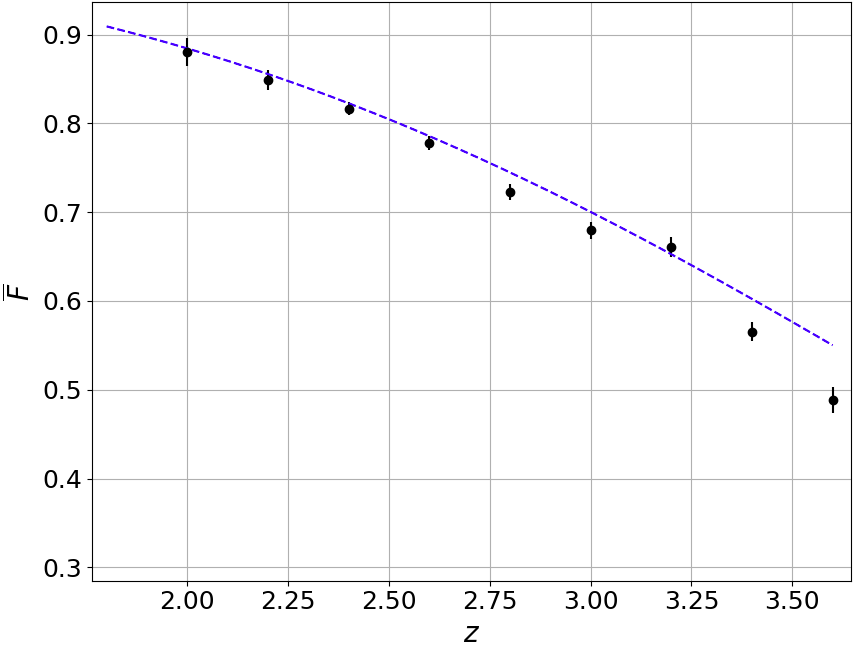
\includegraphics[scale=0.4]{mean_trans}
  \caption{Fraction de flux transmis moyenne en fonction du redshift. Les points noirs donnent la mesure faite par \textcite{Faucher-Giguere2008}. La ligne tiretée bleue donne la paramétrisation de $\overline F(z)$ que nous utilisons dans les mocks.}
  \label{fig:mean_trans}
\end{figure}
En ce qui concerne le terme $\overline F^2$, nous le calculons pour chaque valeur du redshift. Il est donné par l'intégrale du $P^{\mathrm{1D}}$. Pour calculer cette intégrale, nous utilisons $P^{\mathrm{1D}}_{\mathrm{modèle}}$, décrit dans les paragraphes suivants.}



Une fois les paramètres $a$, $b$ et $c$ choisis, nous déterminons le spectre de puissance $P_{s}$ à appliquer à $\delta_{k,s}$ afin d'obtenir le bon $P_{\mathrm{mock}}^{\mathrm{1D}}$.
% Il nous faut $P_{s}$ avant de calculer la prédiction car nous avons besoin de connaître $\sigma_g$.
Nous avons besoin de $P_{s}$ car il nous faut connaître $\sigma_g$, qui lui même requiert $\sigma_s$, pour chaque valeur du redshift afin de calculer la prédiction.
La variance du champ $g = \delta_l + \delta_s + c(z)\eta_{\parallel}$ est donnée par
\begin{equation}
  \label{eq:sigma_g}
  \sigma_g^2(z) = \langle \delta_l^2 \rangle + \langle \delta_s^2 \rangle + c^2(z) \langle \eta_{\parallel}^2 \rangle +
  c(z) \left( \langle \delta_l \eta_{\parallel} \rangle - \langle \delta_l \rangle \langle \eta_{\parallel} \rangle \right)\; .
\end{equation}
Le terme entre parenthèses est la covariance des champs $\delta_l$ et $\eta_{\parallel}$.
% La variance $\sigma_s$ du champ $\delta_s$ est reliée à son spectre de puissance $P_{s}$ par
% \begin{equation}
%   \sigma_s = \frac{1}{d_{pix}N} \left( P_{s}(0) + P_{s}(k_{Ny}) + 2 \sum_{j=1}^{\frac{N}{2} - 1}P_{s}\left(\frac{2 \pi}{d_{pix}N} j\right)\right) \; ,
% \end{equation}
% où $k_{Ny} = \pi / d_{pix} \sim \SI{15.7}{\perh\Mpc}$ est le mode de Nyquist : c'est le mode maximal accessible pour une résolution donnée.
La variance $\sigma_s$ du champ $\delta_s$ est reliée à son spectre de puissance $P_{s}$ par l'équation~\ref{eq:sigma_s}.
Dans le but de calculer $\sigma_s$ puis la prédiction,
nous commençons donc par constuire le spectre de puissance $P^{\mathrm{1D}}_{\mathrm{modèle}}$ sur lequel le $P_{\mathrm{mock}}^{\mathrm{1D}}$ des mocks sera ajusté.
% Tout d'abord, les données provenant de (\#prov On fit les données DR12 sans les oscillations du Si, quel papier ?) sont ajustées dans la gamme $\num{0.2} < k < {2.0} \si{\h\per\Mpc}$. Les oscillations dans le spectre de puissance à une dimension causées par le silicium sont aussi ajustées afin de les retirer et de construire un modèle $P^{\mathrm{1D}}_{modèle}$ sans ces oscillations. La fonction ajustée aux données est définie comme
% \begin{equation}
%   \label{eq:p1d_data}
%   f(k) = \exp(- a k + b + \frac{c}{k + d}) \times f_{Si}(k) \; ,
% \end{equation}
% où $a$, $b$, $c$ et $d$ sont quatres paramètres à ajuster, et $f_{Si}$ est la fonction qui prend en compte les oscillations dues au silicium. La forme choisie permet d'avoir $\log(P^{\mathrm{1D}}_{modèle})$ linéaire à grand k, en accord avec ce qui est mesuré dans les simulations hydrodynamiques \autocite{Arinyo-i-Prats2015}.
% Tout d'abord, les données provenant de (\#prov On fit les données DR12 sans les oscillations du Si, quel papier ?) sont ajustées dans la gamme $\num{0.2} < k < {2.0} \si{\h\per\Mpc}$.
Tout d'abord, le spectre de puissance à une dimension provenant des données DR12 dans lequel les oscillations dues au silicium ont été retirées (Nathalie Palanque-Delabrouille, communication privée) est ajusté dans la gamme $\num{0.2} < k < {2.0} \si{\h\per\Mpc}$.
La fonction ajustée aux données est définie comme
\begin{equation}
  \label{eq:p1d_data}
  % f(k) = \exp(- a k + b + \frac{c}{k + d}) \times f_{\mathrm{Si}}(k) \; ,
  f(k) = \exp(- a k + b + \frac{c}{k + d})  \; ,
\end{equation}
où $a$, $b$, $c$ et $d$ sont quatres paramètres à ajuster.
% La fonction $f_{\mathrm{Si}}$ prend en compte les oscillations dues au silicium.
% Une fois la fonction $f$ de l'équation~\ref{eq:p1d_data} ajustée sur les données, nous utilisons comme modèle pour le spectre de puissance à une dimension la fonction $f$ sans la contribution du silicium $f_{\mathrm{Si}}$. Ceci nous permet de nous affranchir des oscillations dues au silicium dans notre modèle.
La forme choisie pour $f$ permet d'avoir $\log(P^{\mathrm{1D}}_{\mathrm{modèle}})$ linéaire à grand k, en accord avec ce qui est mesuré dans les simulations hydrodynamiques \autocite{Arinyo-i-Prats2015}.
% L'ajustement est fait dans les cinqs bins en redshift $z_1$, $z_2$, $z_3$, $z_4$ et $z_5$.
% L'ajustement est fait dans les bins en redshift \num{2.2} ; \num{2.4} ; \num{2.6} ; \num{2.8} ; \num{3.0} ; \num{3.2} ; \num{3.4} et \num{3.6}.
% Du fait de la résolution $d_{pix} = \SI{0.2}{\perh\Mpc}$ des spectres simulés, nous avons besoin de calculer le  $P_{s}$ jusqu'à $k_{Ny} = \pi / d_{pix} \sim \SI{15.7}{\perh\Mpc}$.
Afin de construire $\delta_s$, nous avons besoin de calculer $P_{s}$ jusqu'à $k_{Ny}$.
Le résultat de l'ajustement sur les données est donc extrapolé de $k = \num{2.0}$ jusqu'à $k = \SI{20}{\h\per\Mpc}$.
Pour les $k$ plus petits que \SI{0.2}{\h\per\Mpc}, nous calculons le $P^{\mathrm{1D}}$ correspondant au modèle de $P^{\mathrm{3D}}$ décrit dans \textcite{Arinyo-i-Prats2015} et ajusté sur des simulations hydrodynamiques.
Ce modèle est défini comme
\begin{equation}
  P(k) = b_{\mathrm{Ly}\alpha}^2 (1 + \beta_{\mathrm{Ly}\alpha} \mu_k^2)^2 P_{\mathrm{L}}(k) D(k, \mu) \; ,
\end{equation}
où $P_{\mathrm{L}}$ est le spectre de puissance linéaire, donné par Camb, et $D(k,\mu)$ représente les déviations par rapport à la théorie linéaire. Le terme $D(k,\mu)$ tend donc vers $1$ à petit $k$. La forme choisie dans \textcite{Arinyo-i-Prats2015} diffère de celle utilisée dans \textcite{McDonald2003}. Cette nouvelle forme permet d'obtenir le bon comportement à petit $k$. Aussi, elle nécessite l'ajustement de moins de paramètres.
$D(k,\mu)$ est donc défini comme
\begin{equation}
  \label{eq:p1d_prats}
  D(k, \mu) = \exp\left[
    \left(q_1 \Delta^2(k) + q_2 \Delta^4(k) \right) \left(1 - \left(\frac{k}{k_v}\right)^{a_v} \mu^{b_v} \right)
    - \left(\frac{k}{k_p} \right)^2 
  \right]
  \; ,
\end{equation}
avec
\begin{equation}
  \Delta^2(k) = \frac{1}{2 \pi^2} k^3 P_L(k) \; .
\end{equation}
Les termes $q_1 \Delta^2(k)$ et $q_2 \Delta^4(k)$ représente l'augmentation de puissance aux petites échelles due aux non-linéarités. L'ajustement que nous utilisons force $q_2 = 0$. Les autres paramètres ajustés sont donnés dans la section ``Planck'' de la table 7 de \textcite{Arinyo-i-Prats2015}.
% Le modèle est calculé pour $z = 2.4$.
Puis, pour chaque valeur du redshift, la forme ajustée aux données et définie dans l'équation~\ref{eq:p1d_data} est prolongée de $k = \SI{0.2}{\h\per\Mpc}$ jusqu'à $k = 0$ par le modèle donné dans l'équation~\ref{eq:p1d_prats}.
% Ce modèle est multiplié par une constante de façon à ce que ce modèle multiplié par cette constante soit égal à l'ajustement fait sur les données à $k = \SI{0.2}{\h\per\Mpc}$.
Pour ce faire, nous calculons le modèle à $z = \num{2.4}$, puis nous le multiplions par une constante, dépendant de la valeur du redshift, de façon à ce que le prolongement en $k = \SI{0.2}{\h\per\Mpc}$ soit continu.
La figure~\ref{fig:p1d_data} montre le modèle ainsi construit. Les données y sont superposées (Nathalie Palanque-Delabrouille, communication privée).
\begin{figure}
  \centering
  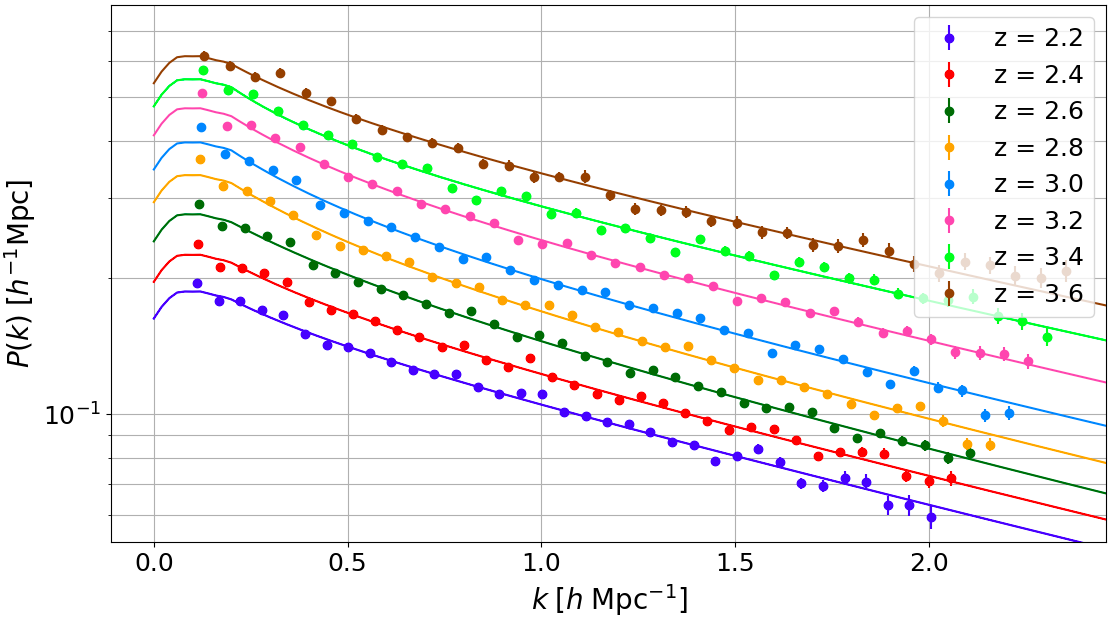
\includegraphics[scale=0.35]{p1d_model_data}
  \caption{Modèle du spectre de puissance à une dimension, pour différentes valeurs du redshift $z$, utilisé dans les mocks. Le modèle, donné par les lignes continues, est ajusté sur les données (Nathalie Palanque-Delabrouille, communication privée), représentées par les points. Ce modèle est décrit dans le texte.}
  \label{fig:p1d_data}
\end{figure}
Pour le bin $z = \num{1.8}$, aucune donnée \lya{} n'est disponible. Nous extrapolons donc le modèle à $z = \num{2.2}$. Nous considérons que la forme du modèle reste la même. Nous considérons aussi que l'évolution en redshift de $z = \num{2.4}$ à $z = \num{2.2}$ est la même jusqu'à $z = \num{1.8}$. Le modèle à $z = \num{1.8}$ est donc donné par
\begin{equation}
  P^{\mathrm{1D}}_{\mathrm{modèle}}(k, z=\num{1.8}) = P^{\mathrm{1D}}_{\mathrm{modèle}}(k, z=\num{2.2}) \left(\frac{P^{\mathrm{1D}}_{\mathrm{modèle}}(k, z=\num{2.2})}{P^{\mathrm{1D}}_{\mathrm{modèle}}(k, z=\num{2.4})} \right)^2 \; .
\end{equation}

Une fois le spectre de puissance modèle défini, nous estimons le spectre de puissance à une dimension $P^{\mathrm{1D}}_{l}$ du champ interpolé $\delta_l + c \eta_{\parallel}$. Nous partons du spectre de puissance fournit par Camb. Nous multiplions ce spectre de puissance par le terme de kaiser $(1 + c \mu_k^2)^2$ puis par le terme $W^2$ représentant l'effet du lissage gaussien (équation~\ref{eq:gauss_smoothing}). Enfin, nous calculons $P^{\mathrm{1D}}_{l}$ grâce à l'équation~\ref{eq:p1d}, en nous restreignant aux $k < k_{max}$. % (\#prov dans p1d\_missing.py, on calcule le p1d avec un cut sur les k. Pourquoi c'est pas un sinus cardinal carré ?).
Une première estimation du spectre de puissance à une dimension $P_{s}^0$ à appliquer à $\delta_{k,s}$ afin d'obtenir le bon $P_{\mathrm{mock}}^{\mathrm{1D}}$ est donnée par
\begin{equation}
  P_{s}^0(k) = P^{\mathrm{1D}}_{\mathrm{modèle}}(k) - P^{\mathrm{1D}}_{l}(k) \; .
\end{equation}
Le spectre de puissance $P_{s}^0$ ainsi construit nous permet d'obtenir un $P_{\mathrm{mock}}^{\mathrm{1D}}$ convenable. Cependant, il reste des différences avec le spectre de puissance modèle. %(\#prov ça vient du fait qu'on applique FGPA ? : oui. mettre un plot du p1d des mocks sans shape tuning et des données ?).
Afin de corriger ces différences, nous ajustons itérativement la forme de $P_{s}$. A chaque itération $n$, nous commençons par générer $\delta_s$ selon $P_{s}^n$. Puis nous calculons le $P_{\mathrm{mock}}^{\mathrm{1D}}$, correspondant à ce $P_{s}^n$. Le $P_{s}^{n+1}$ de l'itération suivante est alors donné par
\begin{equation}
  % P_{s}^{n+1}(k) = P_{s}^{n}(k) \left( 1 + l \left(
  %     \frac{
  %       P_{modèle}^{\mathrm{1D}}(k)
  %     }{
  %       P_{mock}^{\mathrm{1D}}(k)
  %     }
  %       - 1 \right) \right)
  P_{s}^{n+1}(k) = P_{s}^{n}(k)
        \frac{
        P_{\mathrm{modèle}}^{\mathrm{1D}}(k)
      }{
        P_{\mathrm{mock}}^{\mathrm{1D}}(k)
      }
  \; .
\end{equation}
Quelques itérations sont suffisantes pour obtenir un $P_{s}$ qui donne un $P^{\mathrm{1D}}_{\mathrm{mock}}$ en accord avec les données. Nous en effectuons dix pour chaque valeur du redshift.

% A ce stade, nous disposons des informations nécessaires pour générer la prédiction. Nous générons donc la prédiction, puis nous l'ajustons avec le code \picca{}.
A ce stade, nous disposons des informations nécessaires pour calculer la prédiction. Afin de mesurer les paramètres \lya{} prédits, nous générons une pseudo-fonction de corrélation qui suit la prédiction calculée avec le jeu de paramètres. Nous ajustons ensuite cette pseudo-fonction de corrélation avec le code picca, comme nous le ferions avec les mocks.
  Le code picca ajuste les paramètres $b_{\eta, \mathrm{Ly}\alpha}$ et $\beta_{\mathrm{Ly}\alpha}$. Le biais $b_{\mathrm{Ly}\alpha}$ est relié à ces deux paramètres par la relation
  \begin{equation}
    \label{eq:def_bias}
    b_{\mathrm{Ly}\alpha}  = \frac{b_{\eta, \mathrm{Ly}\alpha} f}{\beta_{\mathrm{Ly}\alpha}} \; ,
  \end{equation}
  où $f$ est le taux de croissance des structures.
  Dans la section~\ref{subsec:stab_pars_lya}, nous verrons que les paramètres \lya{} sont corrélés entre eux.
  Ainsi, afin de comparer au mieux la prédiction avec les données, plutôt que de mesurer les paramètres $b_{\eta, \mathrm{Ly}\alpha}$ ou $b_{\mathrm{Ly}\alpha}$ et $\beta_{\mathrm{Ly}\alpha}$, nous mesurons les paramètres $b_{\mathrm{eff},\mathrm{Ly}\alpha}$ et $\beta_{\mathrm{Ly}\alpha}$.
  Le biais effectif $b_{\mathrm{eff},\mathrm{Ly}\alpha}$ est relié au biais et au paramètre RSD du \lya{} par
  \begin{equation}
    \label{eq:def_bias_eff}
    b_{\mathrm{eff},\mathrm{Ly}\alpha} = b_{\mathrm{Ly}\alpha} \sqrt{1 + \frac{2}{3} \beta_{\mathrm{Ly}\alpha} + \frac{1}{5} \beta_{\mathrm{Ly}\alpha}^2} \; .
  \end{equation}
  Il est sensible à l'amplitude de la fonction de corrélation, et est moins corrélé avec $\beta_{\mathrm{Ly}\alpha}$ que l'est $b_{\eta, \mathrm{Ly}\alpha}$ ou $b_{\mathrm{Ly}\alpha}$.
  Enfin, nous mesurons aussi $\overline F$ dans la prédiction, et nous comparons sa valeur à la paramétrisation définie dans l'équation~\ref{eq:mean_trans}.
% Nous comparons la mesure de $b_{\mathrm{Ly}\alpha}$, $\beta_{\mathrm{Ly}\alpha}$ et $\overline F$ à ce qui est mesuré dans les données.
% Toute ces étapes constituent une itération complète de la procédure d'ajustement.
% Dans le cas où les paramètres \lya{} mesurés sur la prédiction ne sont pas en accord avec ce qui est mesuré dans les données, nous relançons une nouvelle itération :
% nous modifions légèrement les paramètres $a$, $b$ et $c$, puis nous recalculons le nouveau $P_{s}^{10}$ afin de générer la nouvelle prédiction. Nous ajustons de nouveau la prédiction avec \picca{} et comparons les valeurs de $b_{\mathrm{eff},\mathrm{Ly}\alpha}$, $\beta_{\mathrm{Ly}\alpha}$ et $\overline F$ mesurées aux données. 
% % Nous relançons ainsi une nouvelle itération : avec les nouveaux paramètres $a$, $b$ et $c$, nous réitérons sur $P_{s}$ avec d'obtenir le nouveau $P_{s}^{10}$, puis nous calculons de nouveau la prédiction, pour l'ajuster avec \picca{}.
% Ces itérations sont répétées dans chaque bin en redshift jusqu'à obtenir des valeurs de $b_{\mathrm{eff},\mathrm{Ly}\alpha}$, $\beta_{\mathrm{Ly}\alpha}$ et $\overline F$ compatibles avec les données.
% Toutes ces étapes constituent une itération complète de la procédure d'ajustement.

L'estimation initiale que nous faisons des paramètres $b$ et $c$ donne des valeurs de $\beta_{\mathrm{Ly}\alpha}$ et $\overline F$ proches de ce qui est mesuré dans les données.
  Cependant, la valeur de $a$ obtenue est trop grande : les paramètres $a$ et $b$ sont estimés à partir des mesures de $P^{\mathrm{1D}}$ et $\overline F$ dans les données.
  Comme nous le verrons dans la section~\ref{subsec:model_donnees}, la présence de HCD dans les données a pour effet d'augmenter le biais effectif mesuré.
  Ainsi, l'estimation du paramètre $a$ est faite avec un $P^{\mathrm{1D}}$ qui possède un biais effectif surestimé.
  Ceci résulte en une valeur de $a$ trop grande qui produit un biais effectif trop grand dans nos mocks.
Nous itérons alors sur les paramètres $a$, $b$ et $c$ : nous diminuons $a$, et si besoin modifions légèrement $b$ et $c$ afin d'affiner les valeurs de $\beta_{\mathrm{Ly}\alpha}$ et $\overline F$ des mocks.  % afin de converger vers les bons $b_{\mathrm{eff},\mathrm{Ly}\alpha}$, $\beta_{\mathrm{Ly}\alpha}$ et $\overline F$.
Puis, nous recalculons le nouveau $P_{s}^{10}$ afin de générer la nouvelle prédiction. Nous ajustons de nouveau la prédiction avec \picca{} et comparons les valeurs de $b_{\mathrm{eff},\mathrm{Ly}\alpha}$, $\beta_{\mathrm{Ly}\alpha}$ et $\overline F$ mesurées aux données. Ces itérations sont faites jusqu'à obtenir des valeurs en accord avec les données.


% Une fois que cette procédure itérative a convergé dans les cinqs bins en redshift, nous ajustons les paramètres $a(z)$, $b(z)$ et $c(z)$ afin d'obtenir une fonction continue de ces paramètres sur $z \in [\num{1.8} \, ; \num{3.6}]$. Les paramètres $\log a(z)$ et $\log b(z)$ sont ajustés par des polynômes de degré 4 de $\log z$. Ceci est fait dans le but d'éviter les valeurs négatives pour $a(z)$, ainsi que les points d'inflection. Le paramètre $c(z)$ est ajusté par un polynôme de degré 4 de $z$.
Une fois que cette procédure itérative a convergé pour les cinq valeurs du redshift, nous interpolons pour avoir des fonctions continues des paramètres $a(z)$, $b(z)$ et $c(z)$ sur $z \in [\num{1.8} \, ; \num{3.6}]$. Pour $a(z)$ et $b(z)$, nous calculons les polynômes de degré quatre de $\log z$ qui passent par les cinq points $\log a(z)$ et $\log b(z)$. Ce choix de fonction est fait dans le but d'éviter des valeurs négatives pour $a(z)$, ainsi que des points d'inflection. Pour le paramètre $c(z)$, nous calculons le polynôme de $z$ qui passe par les cinq points $c(z)$.
La figure~\ref{fig:params} présente les interpolations ainsi obtenues.
\begin{figure}
  \centering
  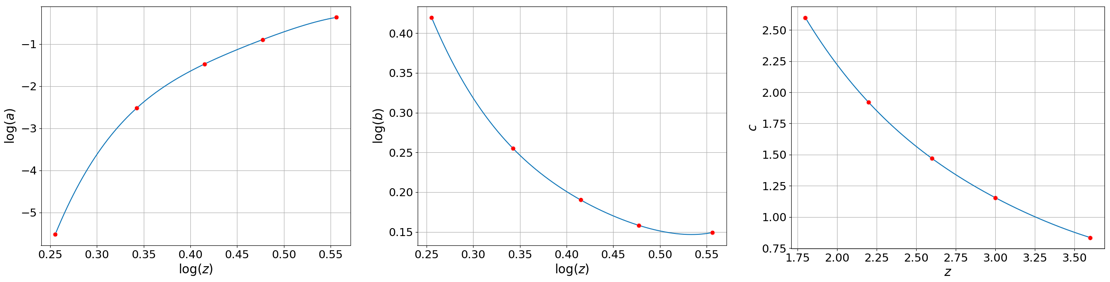
\includegraphics[scale=0.4]{params}
  \caption{Résultat de la procédure d'ajustement des paramètres FGPA.}
  \label{fig:params}
\end{figure}
% Concernant les cinqs spectres de puissance $P_{s}(k)$ construits précédemment dans chaque bin en redshift, nous créons une grille $(k, z)$ sur laquelle nous interpolons cubiquement de ces spectres de puissance
% Les cinq spectres de puissance $P_{s}(k)$ obtenus pour chaque valeur du redshift sont présentés sur la figure~\ref{prov}. Ces spectres sont en très bon accord avec le modèle. Afin d'obtenir $P_{s}(k)$ pour n'importe quel redshift, nous créons une grille $(k, z)$ couvrant $z \in [\num{1.8} \, ; \num{3.6}]$ et $k \in [\num{0} \, ; \num{20}] \si{\h\per\Mpc}$.
% En ce qui concerne les cinq spectres de puissance $P_{s}(k)$ construits précédemment pour chaque valeur du redshift, nous créons une grille $(k, z)$ couvrant $z \in [\num{1.8} \, ; \num{3.6}]$ et $k \in [\num{0} \, ; \num{20}] \si{\h\per\Mpc}$.
\textbf{Les cinq spectres de puissance $P_{s}(k)$ construits précédemment pour chaque valeur du redshift produisent des spectres de puissance $P^{\mathrm{1D}}_{\mathrm{mock}}$ en très bon accord avec le modèle. Les cinq $P^{\mathrm{1D}}_{\mathrm{mock}}$ obtenus pour chaque valeur du redshift sont présentés sur la figure~\ref{fig:p1d_tuning}. Les lignes continues donnent le modèle pour chaque valeur du redshift.
Afin d'obtenir $P_{s}(k)$ pour n'importe quel redshift, nous créons une grille $(k, z)$ couvrant $z \in [\num{1.8} \, ; \num{3.6}]$ et $k \in [\num{0} \, ; \num{20}] \si{\h\per\Mpc}$.}
Puis, $P_{s}(k,z)$ est obtenu via une interpolation cubique sur cette grille. Du fait des très faibles valeurs de $P_{s}$ à grand $k$ et de l'interpolation cubique utilisée, certaines valeurs de l'interpolation sont négatives. Pour chaque redshift de la grille, nous forçons tous les pixels de l'interpolation de $P_{s}$ à zéro pour tous les $k > k_0$, où $k_0$ est le premier $k$ pour lequel l'interpolation est nulle. La figure~\ref{fig:p1dmiss} montre l'interpolation de $P_{s}(k)$ pour différentes valeurs de $z$.
\textbf{Enfin, la figure~\ref{fig:mean_trans_mock} présente la fraction de flux transmise moyenne $\overline F$ en fonction du redshift obtenue avec cette procédure d'ajustement. Celle-ci est mesurée sur une réalisation complète. La ligne en pointillés (orange) montre la paramétrisation définie dans l'équation~\ref{eq:mean_trans}. La mesure faite pour les redshifts proches de \num{3.6} est biaisée par le fait que seuls les pixels proches des quasars participent à cette mesure : la corrélation croisée \lya{}$\times$QSO a pour effet de réduire $F$.}
\begin{figure}
  \centering
  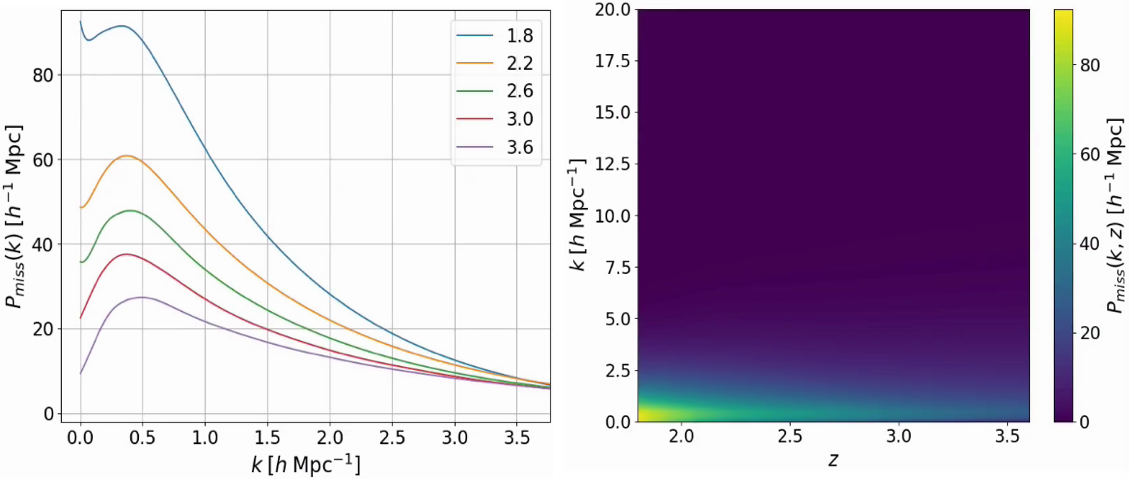
\includegraphics[scale=0.4]{p1dmiss}
  \caption{Gauche : les cinqs spectres de puissance $P_{s}(k)$ ajustés pour chaque valeur du redshift. Droite : interpolation cubique de ces cinqs spectres de puissance sur une grille $(k, z)$.}
  \label{fig:p1dmiss}
\end{figure}
\begin{figure}
  \centering
  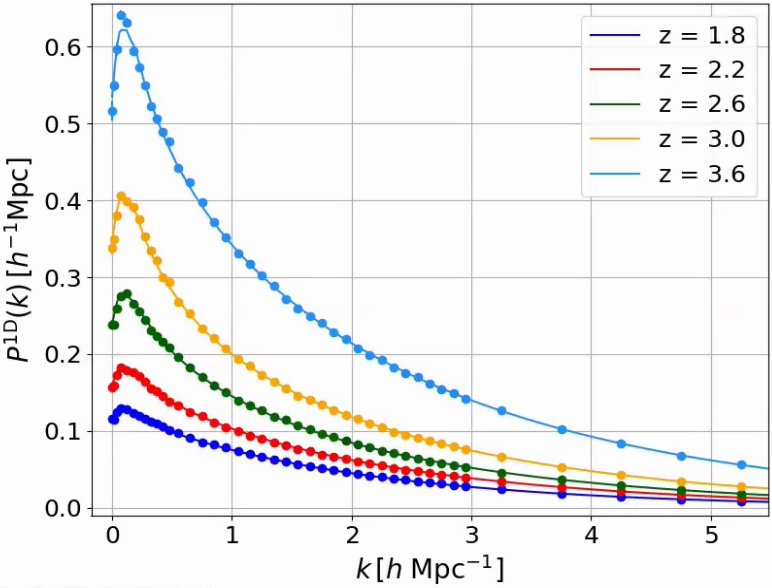
\includegraphics[scale=0.4]{p1d_tuning}
  \caption{Les spectres de puissance $P^{\mathrm{1D}}_{\mathrm{mock}}$ obtenus pour chaque valeur du redshift à la fin de la procédure d'ajustement. Les lignes continues donnent le modèle pour chaque valeur du redshift. Les mocks sont en train bon accord avec le modèle.}
  \label{fig:p1d_tuning}
\end{figure}
\begin{figure}
  \centering
  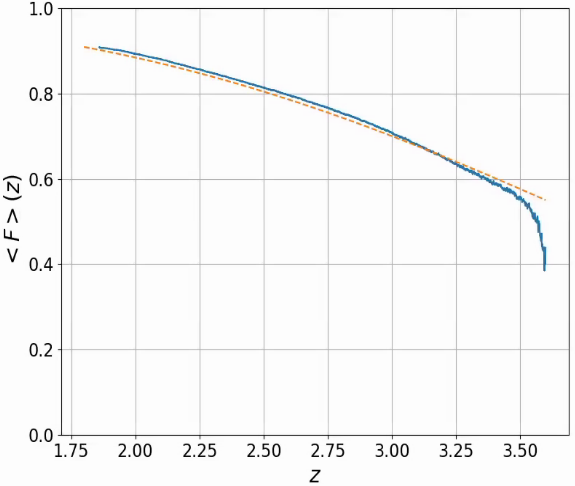
\includegraphics[scale=0.55]{mean_trans_mock}
  \caption{Fraction de flux transmise moyenne $\overline F$ en fonction du redshift mesurée sur une réalisation des mocks. La ligne en pointillés (orange) montre la paramétrisation définie dans l'équation~\ref{eq:mean_trans}.}
  \label{fig:mean_trans_mock}
\end{figure}

\paragraph{}
\textbf{Le résultat de la procédure d'ajustement décrite précédemment a été utilisé pour produire \num{50} réalisations indépendantes des mocks. Nous prévoyons de terminer la post-production des \num{50} autres réalisations pré-produites dans les prochains moins.
  Parmis les \num{50} réalisations produites, \num{30} sont analysées. Le chapitre~\ref{chap:mock_ana} présente cette analyse.}
% Les figures~\ref{prov} présentent les paramètres \lya{} obtenus avec la prédiction (couleur), sur le stack des 100 rea (couleur) et mesuré dans les données (couleur). \#prov montrer biais(z), beta(z), <F>(z) et P1D(z).


\section{Expansion des mocks}
\label{sec:quickquasars}
%Les mocks décrits précédemment produisent un relevé de quasars avec, pour chaque quasar, une forêt d'absorption $F$ variant entre 0 et 1. Afin de simuler complètement la chaîne d'analyse, nous devons ajouter un continuum à ces forêts, puis les inclure dans des spectres simulés. Le code utilisé est le code \texttt{quickquasars}, il est décrit dans \textcite{prov:Alma in prep}. Ce code a pour but de reproduire les données prises avec eBOSS et DESI. Le code simule donc les différents effets propres à chaque instrument comme par exemple la résolution des spectrographes ou le bruit instrumental. Il simule aussi les effets astrophysiques, comme la distribution en magnitude des quasars ou les erreurs de mesure de redshift de ces derniers.

% Une fois les mocks produits, l'idée est d'inclure les forêts simulés dans des spectres synthétiques \#prov mal dit.
Les mocks décrits précédemment produisent un relevé de quasars avec, pour chaque quasar, une forêt d'absorption $F$ variant entre 0 et 1.
Afin de reproduire complètement les données et pouvoir simuler la chaîne d'analyse, nous devons ajouter un continuum à ces forêts, puis ajouter du bruit de mesure.
Le code utilisé pour créer ces spectres synthétiques est le code \texttt{quickquasars}. Il fait parti du package \texttt{desisim}\footnote{https://github.com/desihub/desisim} et est décrit dans \textcite{Gonzalez-Morales}. 

Le continuum des quasars est généré à l'aide du module \texttt{SIMQSO}, du package \texttt{desisim}.
Le modèle utilisé est composé de plusieurs lois de puissance. Ces lois de puissance sont mises bout à bout pour créer le continuum.
Les raies d'émission sont ajoutées en utilisant un modèle fondé sur les spectres des quasars observés par BOSS.
Une option permet d'ajouter des BAL aux spectres de quasars simulés. Nous n'utilisons pas cette option car les spectres présentant un BAL sont retirés des données lors de l'analyse.
Le code permet aussi d'ajouter des HCD et des métaux. Les HCD sont ajoutés dans les spectres aux positions indiquées par le catalogue de HCD que nous générons (voir section~\ref{subsec:hcd)}). Pour chaque HCD, un profil de Voigt, dont la profondeur dépend de la densité de colonne, est créé puis ajouté au spectre.
En ce qui concerne les métaux, ils sont ajoutés en utilisant la transmission du \lya{} : pour chaque métal, la forêt \lya{} est décalée en longueurs d'onde observées par un facteur $\lambda_m / \lambda_{\mathrm{Ly}\alpha}$, où $\lambda_m$ est la longueur d'onde du métal considéré.
Puis, l'absorption est modifiée : 
le flux de chaque absorption est corrigé par un facteur $A_m$, où $A_m$ relie la profondeur optique de la raie d'absorption du métal à la profondeur optique du \lya{} : $\tau_m = A_m \tau_{\mathrm{Ly}\alpha}$. Le paramètre $A_m$ est ajusté afin d'obtenir le bon biais pour chaque métal.
% où $\tau_m$ est la profondeur optique de la raie d'absorption, et $A_m$ un paramètre qui est ajusté pour chaque métal afin d'obtenir le bon biais pour le métal considéré.
Enfin, le code ajoute les spécificités propres à l'instrument ou au relevé (eBOSS ou DESI), comme par exmemple la réponse des spectrographes, le temps d'exposition pour chaque spectre, ou encore la distribution en magnitude des quasars.
La figure~\ref{fig:quickquasars_spectrum} présente le spectre d'un quasar simulé. Un agrandissement de la forêt \lya{} de ce spectre est visible sur la figure~\ref{fig:building_trans}.
% Le graphique du bas montre les régions des forêts \lya{} et \lyb{} en bleu, superposées à la fraction de flux transmis en vert. Cette dernière est multipliée par 30 pour des raisons de visibilité. Le spectre synthétique possède un DLA à $\lambda_{\mathrm{RF}} \sim \SI{1135}{\angstrom}$.

% \begin{figure}
%   \centering
%   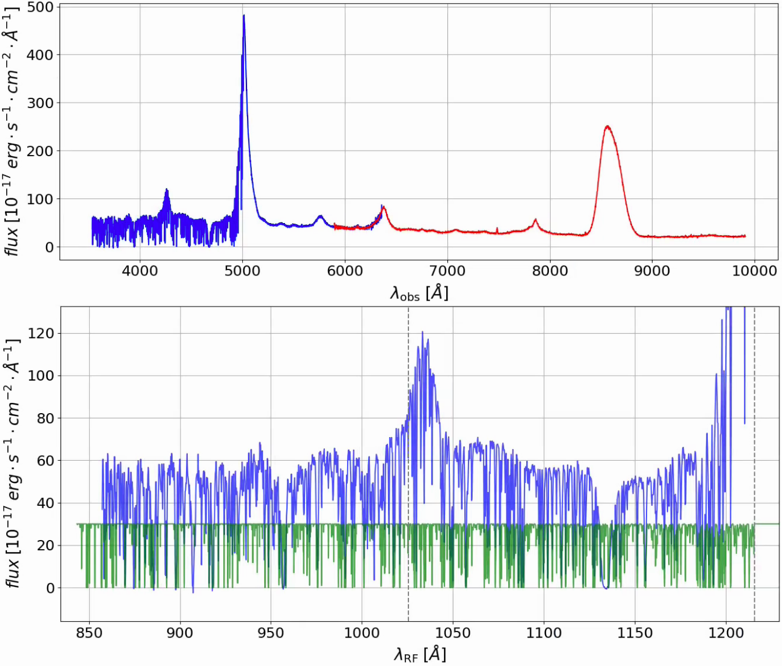
\includegraphics[scale=0.55]{quickquasars_spectra}
%   \caption{Spectre d'un quasar synthétique généré par \texttt{quickqasars}. Le quasar se trouve à un redshift $z = \num{3.121}$. La partie bleue du spectre correspond au spectrographe bleu, la partie rouge correspond au spectrographe rouge. Pour des questions de visibilité, nous avons réduit la zone de recouvrement des deux spectrographes dans cette figure.
%   Le graphique du bas montre le spectre dans les régions des forêts \lya{} et \lyb{} (bleu), superposées à la fraction de flux transmis multipliée par 30 (vert), en fonction de la longueur d'onde au repos. Les pointillés gris indiquent les raies \lya{} et \lyb{}. Un DLA est visible dans le spectre synthétique pour $\lambda_{\mathrm{RF}} \sim \SI{1135}{\angstrom}$.}
%   \label{fig:quickquasars_spectra}
% \end{figure}
\begin{figure}
  \centering
  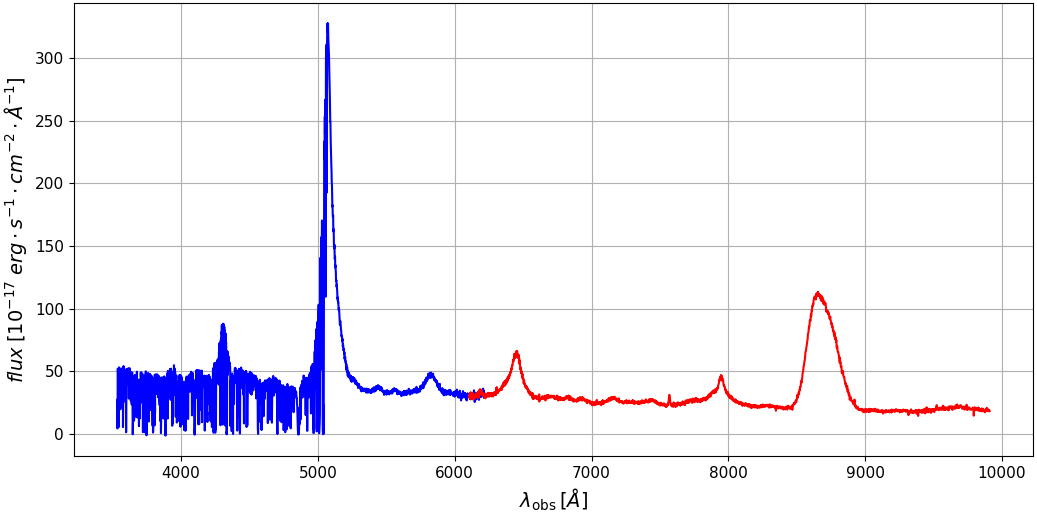
\includegraphics[scale=0.42]{quickquasars_spectrum}
  \caption{Spectre d'un quasar synthétique généré par \texttt{quickqasars}. Le quasar se trouve à un redshift $z = \num{3.167}$. La partie bleue du spectre correspond au spectrographe bleu, la partie rouge correspond au spectrographe rouge. Pour des questions de visibilité, nous avons réduit la zone de recouvrement des deux spectrographes dans cette figure.}
  \label{fig:quickquasars_spectrum}
\end{figure}

\paragraph{}
% A l'aide du code \texttt{quickquasars},nous produisons plusieurs versions différentes des mocks :
Nous produisons plusieurs versions différentes des mocks :
\begin{itemize}
\item les \emph{raw mocks},
\item les mocks \emph{eboss-0.0}, 
\item les mocks \emph{eboss-0.2},
\item les mocks \emph{eboss-0.3}.
\end{itemize}
Les raw mocks sont les mocks bruts, sans l'utilisation de \texttt{quickquasars}. Ces mocks sont analysés en estimant les fonctions de corrélation directement à partir des fichiers de transmission (voir section~\ref{sec:mock_ana}). Ceci nous permet de vérifier la construction des mocks et les différentes fonctions de corrélation, sans que celles-ci soient affectées par l'ajustement du continuum ou les effets astrophysiques et instrumentaux.
Les versions eboss-0.0, eboss-0.2 et eboss-0.3 sont les versions des mocks après avoir utilisé \texttt{quickquasars} pour produire les spectres synthétiques. La version eboss-0.0 correspond à l'ajout du continuum et du bruit. La version eboss-0.2 est la version eboss-0.0 à laquelle les HCD sont ajoutés. La version eboss-0.3 ajoute le continuum, le bruit, les HCD ainsi que les métaux.
Nous présentons l'analyse de ces différentes versions des mocks dans le chapitre suivant.

\textbf{Un point important à noter est que, pour chaque réalisation, les quatre versions présentées ci-dessus sont produites avec le même sous-échantillon de quasars. Ceci facilite la comparaison des différentes versions.}
% En effet, à ce stade nous disposons uniquement d'un relevé de quasars, et pour chacun d'entre deux, une forêt contenant le champ d'absorption $F$ variant entre 0 et 1. Ainsi, afin de simuler complètement les données, nous devons ajouter un continuum à ces forêts, puis les inclure dans des spectres synthétiques. Le code utilisé pour créer ces spectres synthétiques est le code \texttt{quickquasars}. Il fait parti du package \texttt{desisim}\footnote{https://github.com/desihub/desisim} et est décrit dans \textcite{prov}. Ce code utilise 



% \bibliography{../source/library}
% \printbibliography
% \end{document}
